\documentclass[11pt]{article}

% Mathematical typesetting
\usepackage{amsmath}
\usepackage{amsthm}
\usepackage{amssymb}
\usepackage{gensymb}
\usepackage{bbm}
\usepackage{mathrsfs}
\usepackage{centernot}

% Document formatting
\usepackage[utf8]{inputenc}
\usepackage{comment}
\usepackage[shortlabels]{enumitem}
\usepackage{hyperref}
\usepackage{csquotes}
\usepackage{abstract}
\usepackage{array}
\usepackage{float}
\usepackage{caption}

\usepackage{pgfplots}
\usepgfplotslibrary{fillbetween}


%% Remove abstract text
\renewcommand{\abstractname}{\vspace{-\baselineskip}} 

\usepackage[]{geometry}
\geometry{margin=1in, headsep=0.25in}
\newlength{\tabcont}
\setlength{\parindent}{0.0in}
\setlength{\parskip}{0.05in}
\usepackage{framed}
\usepackage[most]{tcolorbox}
\usepackage{xcolor}

\newtheoremstyle{mystyle}{}{}{}{}{\bfseries}{:}{ }{\thmname{#1}\thmnumber{ #2}\thmnote{ (#3)}}
  
\theoremstyle{mystyle}
\newtheorem{thm}{Theorem}[section]
\newtheorem{lm}{Lemma}[section]
\newtheorem{defn}{Definition}[section]
\newtheorem{note}{Note}[section]

\newtheorem{protoexamp}{Example}[section]
\newenvironment{examp}
{\colorlet{shadecolor}{orange!15}\begin{shaded}\begin{protoexamp}}
{\end{protoexamp}\end{shaded}}

\newtheorem{protoexer}{Exercise}[section]
\newenvironment{exer}
{\colorlet{shadecolor}{blue!15}\begin{shaded}\begin{protoexer}}
{\end{protoexer}\end{shaded}}

\newcommand{\0}{\mathbf{0}}

\title{\textbf{Notes on Functional Analysis}}
\author{Henry Smith}
\date{\today}

\begin{document}

\maketitle
\begin{abstract}
    These notes are prepared from my reading of \textit{Introductory Functional Analysis with Applications} by Erwin Kreyszig. They are intended to serve as an aid for my understanding the book content. I do not guarantee their accuracy, and they do not reflect the accuracy of the book.
\end{abstract}

\newpage

\tableofcontents

\newpage

\section{Metric Spaces}\label{secmetric}

\subsection{Metric Spaces: Definition and Examples}

\begin{defn}[Metric Space]\label{metric}
A \textbf{metric space} is a pair $(X, d)$, where $X$ is a set and $d: X \times X \rightarrow \mathbb{R}_+$ is a \textbf{metric} on $X$. The metric $d$ must satisfy the following for all $x, y, z \in X$:
\begin{enumerate}
    \item $d(x, y) = 0 \iff x = y$
    \item $d(x, y) = d(y, x)$ \quad (symmetry)
    \item $d(x, z) \leq d(x, y) + d(y, z)$ \quad (triangle inequality)
\end{enumerate}
\end{defn}

A metric can be thought of as a measure of distance between any two elements $x, y \in X$. To illustrate this point, we provide some examples of metric spaces:

\begin{examp}[The real line $\mathbb{R}$] Let $X = \mathbb{R}$ and $d(x, y) := |x - y|$. Then $(X, d)$ is a metric space. This is our most classical notion of distance.
\end{examp}

\begin{examp}[The complex plane $\mathbb{C}$] Similarly, we let $X= \mathbb{C}$ and $d(x, y) := |x - y|$ for $x, y \in \mathbb{C}$. Recall that for $x = a + bi$, the modulus of $x$ is defined $|x| = \sqrt{a^2 + b^2}$. Then $(X, d)$ is a metric space.

\end{examp}

\begin{examp}[The Euclidean space $\mathbb{R}^n$, unitary space $\mathbb{C}^n$]\label{euclideanunitary}
For $X = \mathbb{R}^n$, we define $d(x, y) := \sqrt{(\xi_1 - \eta_1)^2 + \ldots + (\xi_n - \eta_n)^2 }$, where $x = (\xi_1, \ldots, \xi_n), y = (\eta_1, \ldots, \eta_n) \in \mathbb{R}^n$. $(X, d)$ defines the Euclidean metric space.\newline
Similarly, let $X = \mathbb{C}^n$ and define $d(x, y) := \sqrt{|\xi_1 - \eta_1|^2 + \ldots + |\xi_n - \eta_n|^2}$ for $x, y \in \mathbb{C}^n$. $(X, d)$ defines the unitary metric space.
\end{examp}

These are perhaps the most benign metric spaces that we can conjure from memory. Before presenting more exotic examples of metric spaces, we first discuss a few additional results:

\begin{lm}[Generalized Triangle Inequality]
Let $(X, d)$ be a metric space with $x_1, \ldots, x_n \in X$. Then it holds that
\begin{align*}
    d(x_1, x_n) \leq d(x_1, x_2) + \ldots + d(x_{n-1}, x_n).
\end{align*}
\end{lm}
This follows from an elementary induction argument.

\begin{defn}[Subspace]
Let $(X, d)$ be a metric space and $Y \subset X$ a subset of $X$. Then we can define a metric $\tilde{d}$ on $Y$ according to $\tilde{d} = d|_{Y \times Y}$. This is called the metric induced on $Y$ by $d$.
\end{defn}

The following are important examples of metric spaces that will be relevant throughout the remainder of our studies:
\begin{examp}[The sequence space $\ell^p$]\label{ellp}
For fixed $p \geq 1$, we define the space $\ell^p$ to consist of those complex sequences $x = (\xi_n)_{n=1}^{\infty} \subset \mathbb{C}$ such that
\begin{align*}
    \sum_{n=1}^{\infty}|\xi_n|^p < \infty.
\end{align*}
The metric defined on $\ell^p$ is 
\begin{align*}
    d(x, y) = \left( \sum_{n=1}^{\infty} |\xi_n - \eta_n|^p \right)^{1/p}, \qquad x = (\xi_n), \ y = (\eta_n) \in \ell^p.
\end{align*}
One can verify that indeed $d(x, y) < \infty$ using the \textit{Minkowski inequality}:
\begin{align*}
    \left( \sum_{n=1}^{\infty} | \xi_n + \eta_n|^p  \right)^{1/p} \leq \left( \sum_{n=1}^{\infty} | \xi_n|^p \right)^{1/p} + \left( \sum_{n=1}^{\infty} |\eta_n|^p \right)^{1/p}.
\end{align*}
Then $(\ell^p, d)$ defines a metric space. In the special case of $p = 2$, this is a \textbf{Hilbert space} (see Section \ref{}).
\end{examp}

\begin{examp}[The sequence space $\ell^{\infty}$]\label{ellinfty}
Similar to the space considered in Example \ref{ellp}, we let $\ell^{\infty}$ be the set of all bounded sequences in $\mathbb{C}$. That is,
\begin{align*}
    \ell^{\infty} = \{ x = (\xi_n) \subset \mathbb{C} \ | \ | \xi_n | \ \leq c_x \ \text{for some $c_x \in \mathbb{R}_+$} \}.
\end{align*}
The metric we define on $\ell^{\infty}$ is $d(x, y) = \sup_{n \in \mathbb{N}} |\xi_n - \eta_n |$. $(\ell^{\infty}, d)$ defines a metric space.
\end{examp}

\begin{examp}[The function space $C{[a,b]}$]\label{contfun}
Let $X$ be the set of all real-valued continuous functions defined on the interval $[a, b]$. Then for each $x(t), y(t) \in X$, we define the metric $d(x, y) := \max_{t \in [a, b]} | x(t) - y(t) |$.\newline 
One should notice that we use \enquote{max} rather than \enquote{sup} in our definition of the metric $d$. This is because $f(t) = |x(t) - y(t)|$ is continuous on the closed interval $[a, b]$ and thus attains its maximum on this interval (the Weierstrass Extreme Value Theorem).\newline
This defines the metric space $C[a, b]$.
\end{examp}

\begin{examp}[The discrete metric space]\label{discretemetric}
For any set $X$, define the metric $d$ such that
\begin{align*}
    d(x, y) = 
    \begin{cases}
    1 & \text{if $x=y$} \\
    0 & \text{otherwise}
    \end{cases}.
\end{align*}
Then $(X, d)$ is called the \textbf{discrete metric space}.
\end{examp}

\begin{exer}
If $A$ is the subspace of $\ell^{\infty}$ consisting of all zeros and ones, what is the induced metric on $X$?\newline
The induced metric $\tilde{d}$ on $A$ is the discrete metric (see Example \ref{discretemetric}).
\begin{proof}
Let $x = (\xi_n), y = (\eta_n) \in A$. Then if $x \neq y$, it must be the case that $|\xi_j - \eta_j| = 1$ for some $j \in \mathbb{N}$. By the definition of $(\ell^{\infty}, d)$, this implies $\tilde{d}(x, y) = 1$. Also, by the properties of a metric space, we know $\tilde{d}(x, x) = 0$. We deduce that $\tilde{d}$ is the discrete metric.
\end{proof}
\end{exer}

\begin{exer}\label{intmetric}
Show that a metric on the space $X$ from Example \ref{contfun} is 
\begin{align*}
    \tilde{d}(x, y) = \int_a^b |x(t) - y(t)| dt.
\end{align*}

\begin{proof}
First, notice that since $x, y \in X$, then $|x - y| \in X$. That is, $|x(t) - y(t)|$ is continuous over $[a, b]$, and is thus Riemann integrable. This means that $\tilde{d}$ is well-defined. Similarly, we have
\begin{enumerate}
    \item $|x(t) - y(t)| \geq 0, \ t \in [a, b] \implies \tilde{d}(x, y) = \int_a^b |x(t) - y(t)| dt \geq 0$
    \item $|x(t) - y(t)| \leq c, \ \forall t \in [a, b]$ for some $c \in \mathbb{R}_+$ $\implies \tilde{d}(x, y) \leq c \cdot (b -a) \in \mathbb{R}_+$
\end{enumerate}
Therefore, it is indeed the case that $\tilde{d}: X \times X \rightarrow \mathbb{R}_+$.\newline
To verify axiom (1), we clearly see that $x = y$ implies $\tilde{d}(x, y) = 0$. For the opposite implication, suppose $x(t_0) \neq y(t_0)$ for some $t_0 \in [a, b]$. Without loss of generality, suppose $t_0 \notin \{a, b\}$. Then by the continuity of $x$ and $y$, this implies that $|x(t) - y(t)| > 0$ for all $t \in [t_0 - \varepsilon, t_0 + \varepsilon] \subseteq [a, b]$, where $\varepsilon > 0$ is chosen to be sufficiently small. Accordingly, we have
\begin{align*}
    &\tilde{d}(x, y) = \underbrace{\int_a^{t_0 - \varepsilon} |x(t) - y(t)| dt}_{\geq 0} + \underbrace{\int_{t_0 - \varepsilon}^{t_0 + \varepsilon} |x(t) - y(t)| dt}_{> 0} + \underbrace{\int_{t_0 - \varepsilon}^{b} |x(t) - y(t)| dt}_{\geq 0}\\
    \implies&\tilde{d}(x, y) > 0.
\end{align*}
Symmetry (2) of the metric $\tilde{d}$ follows from the properties of the absolute value.\newline
Finally, to prove the triangle inequality (3), we have that for $x, y, z$ continuous functions on $[a, b]$
\begin{align*}
    \tilde{d}(x, z) &= \int_a^b | x(t) - z(t) | dt \leq \int_a^b \bigg( | x(t) - y(t) | + | y(t) - z(t) |\bigg) dt\\
    &= \int_a^b | x(t) - y(t) | dt + \int_a^b | y(t) - z(t) | dt\\
    &= \tilde{d}(x, y) + \tilde{d}(y, z).
\end{align*}
\end{proof}
\end{exer}

\begin{exer}
Show that nonnegativity of a metric follows from axioms (1) - (3).

\begin{proof}
Let $(X, d)$ be a metric space and $x, y \in X$ arbitrary points. Then by (3) we have
\begin{align*}
    d(x, x) \leq d(x, y) + d(y, x).
\end{align*}
Property (1) implies
\begin{align*}
    0 \leq d(x, y) + d(y, x).
\end{align*}
And property (2) implies
\begin{align*}
    0 \leq 2d(x, y) \iff 0 \leq d(x, y).
\end{align*}
\end{proof}
\end{exer}

\begin{exer}\label{sequencespaces}
Define $s$ to be the space of all (bounded or unbounded) sequences of complex numbers and the metric $d$ defined by
\begin{align*}
    d(x, y) = \sum_{n=1}^{\infty} \frac{1}{2^n} \frac{|\xi_n - \eta_n|}{1 + |\xi_n - \eta_n|}, \qquad x = (\xi_n), \ y= (\eta_n) \in s.
\end{align*}
Show that we can obtain another metric by replacing $(1/2^n)$ with $(\mu_n), \ \mu_n > 0$ such that $\sum \mu_n$ converges.
\begin{proof}
First, we point out that $\mu_n \cdot \frac{|\xi_n - \eta_n|}{1 + |\xi_n - \eta_n|} \geq 0$ for each $n \in \mathbb{N}$, and so $\tilde{d}(x, y) = \sum_{n=1}^{\infty} \mu_n \cdot \frac{|\xi_n - \eta_n|}{1 + |\xi_n - \eta_n|} \geq 0$. Also we notice that $\mu_n \cdot \underbrace{\frac{|\xi_n - \eta_n|}{1 + |\xi_n - \eta_n|}}_{ < 1} < \mu_n$ for each $n \in \mathbb{N}$, and so $\tilde{d}(x, y) = \sum_{n=1}^{\infty} \mu_n \cdot \frac{|\xi_n - \eta_n|}{1 + |\xi_n - \eta_n|} < \sum_{n=1}^{\infty} \mu_n < \infty$.\newline
Now, for (1) we have 
\begin{align*}
    &\tilde{d}(x, y) = 0 \iff \sum_{n=1}^{\infty} \underbrace{\mu_n \cdot \frac{|\xi_n - \eta_n|}{1 + |\xi_n - \eta_n|}}_{\geq 0} = 0 \iff \mu_n \cdot \frac{|\xi_n - \eta_n|}{1 + |\xi_n - \eta_n|} = 0, \ n \in \mathbb{N}\\
    \iff& \frac{|\xi_n - \eta_n|}{1 + |\xi_n - \eta_n|} = 0, \ n \in \mathbb{N} \iff x = y.
\end{align*}
(2) follows simply from the properties of the modulus function.\newline
Finally, for the triangle inequality (3), we let $z = (\gamma_n) \in s$ and use the result from pp. 10 - 11:
\begin{align*}
    &\frac{|\xi_n - \gamma_n|}{1 + |\xi_n - \gamma_n|} \leq \frac{|\xi_n - \eta_n|}{1 + |\xi_n - \eta_n|} + \frac{|\eta_n - \gamma_n|}{1 + |\eta_n - \gamma_n|}, \quad n \in \mathbb{N}\\
    \iff&\mu_n \cdot \frac{|\xi_n - \gamma_n|}{1 + |\xi_n - \gamma_n|} \leq \mu_n \cdot \frac{|\xi_n - \eta_n|}{1 + |\xi_n - \eta_n|} + \mu_n \cdot \frac{|\eta_n - \gamma_n|}{1 + |\eta_n - \gamma_n|}, \quad n \in \mathbb{N}\\
    \implies& \sum_{n=1}^{\infty} \mu_n \cdot \frac{|\xi_n - \gamma_n|}{1 + |\xi_n - \gamma_n|} \leq \sum_{n=1}^{\infty} \mu_n \cdot \frac{|\xi_n - \eta_n|}{1 + |\xi_n - \eta_n|} + \sum_{n=1}^{\infty} \mu_n \cdot \frac{|\eta_n - \gamma_n|}{1 + |\eta_n - \gamma_n|}\\
    \iff& \tilde{d}(x, z) \leq \tilde{d}(x, y) + \tilde{d}(y, z).
\end{align*}
We deduce $(s, \tilde{d})$ is a metric space.
\end{proof}
\end{exer}

\begin{exer}
The \textbf{diameter} $\delta(A)$ of a nonempty set $A$ in a metric space $(X, d)$ is defined to be 
\begin{align*}
    \delta(A) = \sup_{x, y\in A} d(x, y).
\end{align*}
$A$ is said to be \textbf{bounded} if $\delta(A) < \infty$. Prove each of the following:
\begin{enumerate}
    \item $A \subset B$ implies $\delta(A) \leq \delta(B)$.
    \item $\delta(A) = 0 \iff$ $A$ consists of a single point.
\end{enumerate}

\begin{proof}
(1) This follows from the properties of the the supremum. Namely, 
\begin{align*}
    &C_1=\{d(x, y) \ | \ x, y \in A \} \subset C_2=\{d(x, y) \ | \ x, y \in B \}\\
    \implies& \sup C_1 \leq \sup C_2\\
    \iff& \delta(A) \leq \delta(B).
\end{align*}
(2) 
\begin{align*}
    &\delta(A) = 0 \iff \sup_{x, y\in A} d(x, y) = 0 \iff d(x, y) = 0, \ \forall x, y \in A\\
    &\iff\text{A consists of a single point}
\end{align*}
\end{proof}
\end{exer}

\begin{exer}
The \textbf{distance} $D(A, B)$ between two nonempty subsets $A$ and $B$ of a metric space $(X, d)$ is defined to be 
\begin{align*}
   D(A, B) = \inf_{\substack{a \in A\\b \in B}} d(a, b). 
\end{align*}
Show each of the following:
\begin{enumerate}
    \item $D$ does \textit{not} define a metric on the power set of $X$.
    \item If $A \cap B \neq \varnothing$, then $D(A, B) = 0$. What about the converse?
\end{enumerate}

\begin{proof}
(1) Let $P, Q \in 2^X$ such that $P \neq Q$ and $P \cap Q \neq 
\varnothing$. Notice that $d$ is a metric, and so $d(p, q) \geq 0, \ \forall p \in P, \ \forall q \in Q$. This implies $D(P, Q) \geq 0$. Moreover, $P \cap Q \neq \varnothing$ implies $D(P, Q) \leq 0$. Altogether, we have shown $D(P, Q) = 0$ but $P \neq Q$. Therefore, we conclude $D$ does not define a metric.\newline
(2) Since $A \cap B \neq \varnothing$, then $0 \in \{ d(a, b) \ | \ a \in A, \ b \in B\}$. This tells us that $D(A, B) \geq 0$. And by our argument from (1), $d(a, b) \geq 0, \ \forall a \in A, \ \forall b \in B$, which implies $D(A, B) = \inf_{\substack{a \in A\\b \in B}} d(a, b) \geq 0$. We conclude $D(A, B) = 0$.\newline
The converse is not true. Consider the Euclidean metric space $(\mathbb{R}^2, d)$. Let $A = \{(x, 0) \ | \ x > 0 \}$ be the positive $x$-axis and $B = \{(x, y) \ | \ x >0, \ y \geq x^{-1} \}$ the region bounded by the curve $y = x^{-1}$. Since $x^{-1} > 0$ for every $x > 0$, then $A \cap B = \varnothing$. Consider the sequence $(a_n) \subset A$ defined $a_n = (n, 0)$ as well as the sequence $(b_n) \subset B$ defined $b_n = (n, n^{-1})$. Then $d(a_n, b_n) = n^{-1}$ for all $n \in \mathbb{N}$, which proves that $D(A, B) = \inf_{\substack{a \in A\\b \in B}} d(a, b) \leq 0$. By nonnegativity of the metric $d$, we conclude $D(A, B) = 0$ but $A \cap B = \varnothing$.
\end{proof}

% Add plot
\begin{center}
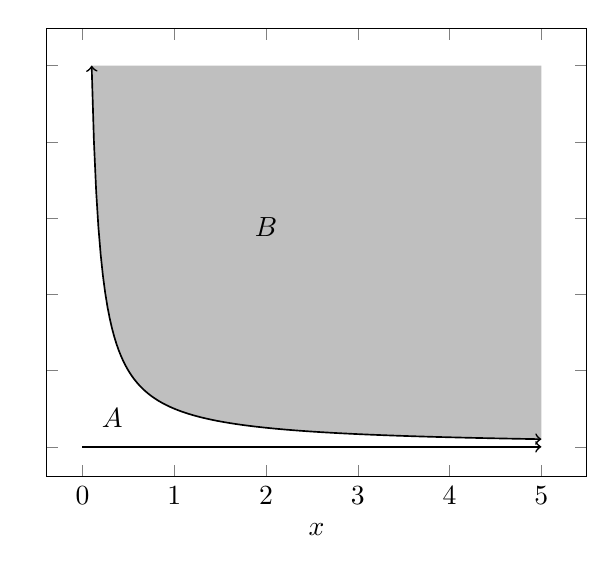
\begin{tikzpicture}
\begin{axis}[samples=200, xlabel={$x$}, yticklabels={}]
\addplot[<->, semithick][name path=f, domain=.1:5] {1/x};
\node[label={$B$}] at (axis cs:2,5) {};
\path[name path=axis] (axis cs:0.1,10) -- (axis cs:5,10);
\addplot[gray!50] fill between[of=f and axis];
\node[circle, label={45:$A$}] at (axis cs:0,0) {};
\draw[->, semithick] (axis cs:0,0) -- (axis cs:5,0);
\end{axis}
\end{tikzpicture}
\end{center}
\end{exer}

\newpage
\begin{exer}\label{pttoset}
The \textbf{distance} $D(x, B)$ from a point $x$ to a nonempty subset $B$ of a metric space $(X, d)$ is defined to be
\begin{align*}
    D(x, B) = \inf_{b \in B} d(x, b).
\end{align*}
Show that for any $x, y \in X$, $|D(x, B) - D(y, B)| \leq d(x, y)$.
\begin{proof}
For each element $b \in B$, it holds that $d(x,b) \leq d(x, y) + d(y, b)$ by the triangle inequality. Consequently, we get the inequality 
\begin{align*}
    \inf_{b \in B} d(x, b) \leq d(x, y) + \inf_{b \in B} d(y, b) \iff D(x, B) - D(y, B) \leq d(x, y).
\end{align*}
By starting with $d(y, b) \leq d(y, x) + d(x, b)$, we similarly have $D(y, b) - D(x, b) \leq d(x, y)$. And so we conclude $|D(x, B) - D(y, B)| \leq d(x, y)$, as desired.
\end{proof}
\end{exer}

\subsection{Set Theory, Continuity, and Separability}

\subsubsection{Set Theory}\label{settheory}

\begin{defn}[Ball and sphere]
Let $(X, d)$ be a metric space. Given a point $x_0 \in X$ and a real number $r > 0$, we define three sets:
\begin{enumerate}
    \item \textbf{Open ball}: $B_r(x_0) = \{x \in X | d(x, x_0) < r \}$
    \item \textbf{Closed ball}: $\tilde{B}_r(x_0) = \{x \in X | d(x, x_0) \leq r \}$
    \item \textbf{Sphere}: $S_r(x_0) = \{x \in X | d(x, x_0) = r \}$
\end{enumerate}
\end{defn}

% Add plot
\begin{figure}[H]
\begin{center}
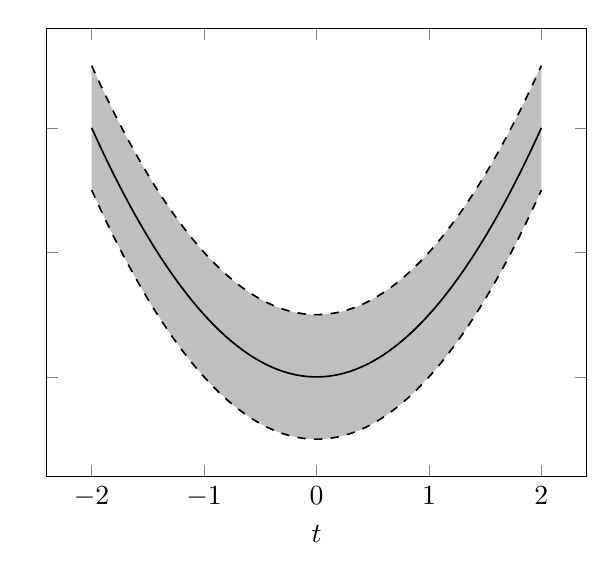
\begin{tikzpicture}
\begin{axis}[samples=200, xlabel={$t$}, yticklabels={}, yticklabels={}]
\addplot[semithick][name path=f, domain=-2:2] {x^2};
\addplot[semithick, dashed][name path=g, domain=-2:2] {x^2 -1};
\addplot[semithick, dashed][name path=h, domain=-2:2] {x^2 +1};
\addplot[gray!50] fill between[of=g and h];
\end{axis}
\end{tikzpicture}
\end{center}
\caption*{The open unit ball $B_{r=1}(x)$ for $x(t) = t^2$ in the function space $C[-2, 2]$}
\end{figure}


\begin{defn}[Open set, closed set]
A subset $M$ of a metric space $X$ is said to be \textbf{open} if it contains a (open) ball about each of its points. A subset $K$ is said to be \textbf{closed} if its complement $X \setminus K$ is open.
\end{defn}

\begin{examp}\label{emptyopen}
In an arbitrary metric space $X$, the subsets $\varnothing$ and $X$ are both open and closed.
\end{examp}

\begin{examp}
In a discrete metric space $X$, every subset is both open and closed.
\begin{proof}
It suffices to show that for each $M \in 2^X$, then $M$ is open. One will recall that $\varnothing$ is open from Exercise \ref{emptyopen}, so we suppose $|M| > 0$. Let $m \in M$ be an arbitrary point in $M$. Then for each $r \in (0, 1]$, the open ball $B_r(x_0) = \{m \}$ is contained in the set $M$. This proves that $M$ is open, and we conclude that every subset of a discrete metric space is both open and closed.
\end{proof}
\end{examp}

\begin{defn}
Let $X$ be a metric space and $M$ a (nonempty) subset of $X$. Then $x_0 \in M$ is an \textbf{interior point} of the set $M$ if there exists some $r > 0$ such that $B_r(x_0) \subset M$. The \textbf{interior} of $M$, denoted $\text{Int}(M)$ is the set of all interior points of $M$.
\end{defn}

Immediately, we see that every point of an open set $M$ is an interior point, per our definition of an open set, and so $\text{Int}(M) = M$. Moreover, we have the following result which explains why we care about set interiors:

\begin{thm}\label{interior}
Let $X$ be a metric space and $M$ a nonempty subset of $X$. Then $\text{Int}(M)$ is the largest open set contained in $M$.
\end{thm}
\begin{proof}
First we prove that $\text{Int}(M)$ is a subset of $M$ and is open. By our definition, it is clear that $\text{Int}(M) \subseteq M$. Toward contradiction, suppose that $\text{Int}(M)$ is not open, meaning there exists some $x_0 \in \text{Int}(M)$ such that $B_r(x_0) \not\subset \text{Int}(M)$ for each $r > 0$. But this mean that $B_r(x_0) \not\subset M$ for each $r > 0$, which contradicts our assumption that $x_0 \in \text{Int}(M)$.\newline
We proceed to show that $\text{Int}(M)$ is the largest open set contained in $M$. Let $U$ be an arbitrary open set contained in $M$. Then for each $u \in U$ we have $u \in B_r(u) \subset U \subseteq M$, which implies $u \in \text{Int}(M)$. And so we conclude $U \subseteq \text{Int}(M)$.
\end{proof}

Having formally defined an open set for a metric space $(X, d)$, we give a more general notion of a space that satisfies the properties of open sets:
\begin{defn}
A \textbf{topological space} $(X, \mathscr{F})$ is a set $X$ and a collection $\mathscr{F}$ of subsets of $X$ such that $\mathscr{F}$ satifies the following axioms:
\begin{enumerate}
    \item $\varnothing, X \in \mathscr{F}$ 
    \item $\{F_n\}_{n \in \mathcal{I}} \subseteq \mathscr{F} \implies \bigcup_{n \in \mathcal{I}} F_n \in \mathscr{F}$ \quad ($\mathscr{F}$ is closed under arbitrary unions)
    \item $\{F_n\}_{n=1}^N \subseteq \mathscr{F} \implies \bigcap_{n=1}^N F_n \in \mathscr{F}$ \quad ($\mathscr{F}$ is closed under finite intersections)
\end{enumerate}
\end{defn}

It is evident that each metric space $X$ is a topological space with $\mathscr{F}$ the collection of all open subsets of $X$.

\begin{note}
One should be careful in recognizing that open sets, and thus topological spaces, \textit{are not closed under countable intersections}. For a straightforward counterexample, let $(\mathbb{R}, d)$ be the Euclidean metric space and take $\{F_n \}_{n \in \mathbb{N}}$ where each $F_n := (-n^{-1}, n^{-1})$ is an open set. Then $\cap_{n \in \mathbb{N}} F_n = \{ 0 \}$ is not open.
\end{note}

\begin{defn}
Let $X$ be a metric space and $M$ a (nonempty) subset of $X$. Then a point $x$ of $X$, which may or may not be a point of $M$, is called an \textbf{accumulation point} or \textbf{limit point} of $M$ if for every $\varepsilon > 0$, $B_{\varepsilon}(x)$ contains a point $m_{\varepsilon}\in M$ distinct from $x$. The set consisting of the points of $M$ and the limit points of $M$ is called the \textbf{closure} of $M$ and is denoted by $\bar{M}$.
\end{defn}

\begin{thm}
Let $X$ be a metric space and $M$ a nonempty subset of $X$. Then $\bar{M}$ is the smallest closed set containing $M$.
\end{thm}
\begin{proof}
Similar to the structure of our proof of Theorem \ref{interior}, we first show that $\bar{M}$ contains $M$ and is closed. The first statement is a consequence of the definition of the closure. As for the latter, let $x_0 \in X \setminus \bar{M}$ be an arbitrary point. Suppose towards contradiction that there exists no $\varepsilon > 0$ such that $B_{\varepsilon}(x_0) \subset X \setminus \bar{M}$. Then for every $\varepsilon > 0$, there exists some $m_{\varepsilon} \in M$ such that $m_{\varepsilon} \in B_{\varepsilon}(x_0)$. However, this means that $x_0$ is a limit point of the set $M$, and so $x_0 \in \bar{M}$, a contradiction.\newline
Now we show that $\bar{M}$ is the smallest closed set containing $M$. In particular, let us consider an arbitrary closed set $U$ containing $M$. And choose an arbitrary point $m_0 \in \bar{M}$. Suppose towards contradiction that $m_0 \notin U \implies m_0 \in X \setminus U$. Also notice that since $M \subseteq U$, then the point $m_0$ cannot be contained in $M$. Thus, $m_0$ must be a limit point of $M$. This, however, is a contradiction, since it implies that $B_{\varepsilon}(m_0)$ contains a point $m_{\varepsilon} \in M \subseteq U$ for each $\varepsilon > 0$, and so $X \setminus U$ cannot be open. Thus, it must be the case that $\bar{M} \subseteq U$ for each closed set $U$ containing $M$.
\end{proof}

\subsubsection{Continuity}

\begin{defn}[Continuous mapping]
Let $(X, d)$ and $(Y, \tilde{d})$ be metric spaces. A mapping $T: X \longrightarrow Y$ is said to be \textbf{continuous at a point} $x_0 \in X$ if for every $\varepsilon > 0$, there exists some $\delta > 0$ such that
\begin{align*}
    d(x, x_0) < \delta \quad \implies \quad \tilde{d}(Tx, Tx_0) < \varepsilon.
\end{align*}
$T$ is said to be \textbf{continuous} if it is continuous at all points $x \in X$.
\end{defn}

Continuous mappings have an important connection with open sets as summarized by the following theorem:
\begin{thm}[Continuous Mapping]\label{continuousmapping}
A mapping $T$ of a metric space $X$ into a metric space $Y$ is continuous if and only if the inverse image of any open subset of $Y$ is an open subset of $X$.
\end{thm}
\begin{proof}
$\implies$ Suppose $T$ is continuous, and let $A$ be any open subset of $Y$.
Further, let $B = T^{-1}A$ be the inverse image of $A$. Consider an arbitrary $b_0 \in B$. Then $Tb_0 \in A$. By assumption that $A$ is open, there exists some $\varepsilon > 0$ such that $B_{\varepsilon}(Tb_0) \subset A$. And since $T$ is continuous, there exists some $\delta > 0$ such that $d(b, b_0) < \delta \implies \tilde{d}(Tb, Tb_0) < \varepsilon$. But because $B_{\varepsilon}(Tb_0) \subset A$, this implies that the ball $B_{\delta}(b_0)$ is contained in $B$.\newline
$\impliedby$ Conversely, suppose the inverse image of any open subset of $Y$ is an open subset of $X$. Let us take $x_0 \in X$ to be arbitrary. Then for each $\varepsilon > 0$, $B_{\varepsilon}(Tx_0)$ is an open set. By our assumption, this means that the inverse image of  $B_{\varepsilon}(Tx_0)$, denoted $A$, is open. Consequently, by the definition of $A$ an open set, there exists some $\delta > 0$ such that $B_{\delta}(x_0) \subset A$. Thus we conclude $d(x, x_0) < \delta \implies \tilde{d}(Tx, Tx_0) < \varepsilon$.
\end{proof}

\subsubsection{Separability}
The set theory we have built up in Section \ref{settheory} leads us to the important concept of dense subsets and separable spaces which will be important throughout the remainder of our studies:
\begin{defn}[Dense set, separable space]
A subset $M$ of a metric space $X$ is said to be \textbf{dense} in $X$ if $\bar{M} = X$. $X$ is said to be \textbf{separable} if it has a \textit{countable} subset which is dense in $X$.
\end{defn}

Consequently, if $M$ is dense in $X$, then every ball in $X$ (with nonzero radius), no matter how small, will contain a point of $M$.

\begin{examp}[Weierstrass Approximation Theorem]\label{weierstrass}
The set of polynomial functions defined on the interval $[a, b] \subset \mathbb{R}$ is dense in the metric space $C[a, b]$.\footnotemark
\end{examp}\footnotetext{My favorite proof of the Weierstrass Approximation Theorem is that which relies upon \href{https://en.wikipedia.org/wiki/Fej\%C3\%A9r\%27s_theorem}{Fejer's Theorem}.}

\begin{examp}
$\mathbb{R}$ is separable.
\begin{proof}
$\mathbb{Q}$ is a countable, dense subset of $\mathbb{R}$.
\end{proof}
\end{examp}

\begin{examp}
$\mathbb{C}$ is separable.
\end{examp}

\begin{examp}
$\ell^{\infty}$ is \textbf{not} separable. $\ell^P$ is separable for $1 \leq p < \infty$.
\begin{proof}
We prove that $\ell^p$ is separable.\newline
Let us define the set 
\begin{align*}
    M_n = \{ (\eta_1, \ldots, \eta_n, 0, 0,\ldots ) \ | \  \eta_i \in \mathbb{Q} \ \text{for} \ 1 \leq i \leq n\}
\end{align*}
which consists of those sequences whose first $n$ terms are rational and remaining terms are zero. Each of these sequences is in $\ell^p$ since it only has finitely many nonzero terms. Note that $M_n$ is countable since it is equal to the Cartesian product of countable sets.\newline
From here the set
\begin{align*}
    M = \bigcup_{n \in \mathbb{N}} M_n
\end{align*}
is countable because it is a countable union of countable sets.\newline
We claim that $M$ is dense in $\ell^{p}$. To prove this, take an arbitrary element $x = (\xi_1, \xi_2, \ldots) \in \ell^p$. Then for each $\varepsilon > 0$, there must exist some $N_{\varepsilon}$ such that $\sum_{n > N_{\varepsilon}} |\xi_i|^p < \frac{\varepsilon^p}{2}$ (by definition of the space $\ell^p$). And since $\mathbb{Q}$ is dense in the Euclidean metric space $\mathbb{R}$, for each $\xi_n$, $1 \leq n \leq N_{\varepsilon}$ there exists an $\eta_n$ such that $|\xi_n - \eta_n| < \frac{\varepsilon^p}{2^{n+1}}$.\newline
Let us define $w = (\eta_1, \ldots, \eta_n, 0, 0 \ldots,) \in M$. Then we have that
\begin{align*}
    d(x, w) &= \left( \sum_{n=1}^{\infty} |\xi_n - \eta_n|^p \right)^{1/p}
    = \left( \sum_{n=1}^{N_{\varepsilon}} |\xi_n - \eta_n|^p + \sum_{n > N_{\varepsilon}} |\xi_n|^p \right)^{1/p}\\
    &\leq \left( \frac{\varepsilon^p}{2} + \frac{\varepsilon^p}{2} \right)^{1/p} = \varepsilon.
\end{align*}
Because $\varepsilon > 0$ was chosen arbitrarily, we deduce that $M$ is indeed dense in $\ell^p$ for each $1 \leq p < \infty$, and so $\ell^p$ is separable.
\end{proof}
\end{examp}

\begin{exer}
Consider $C[0, 2\pi]$ and determine the smallest $r$ such that $y \in \tilde{B}_r(x)$, where $x(t) = \sin(t)$ and $y(t) = \cos(t)$.\newline
First, we comment that
\begin{align*}
    y \in \tilde{B}_r(x) \iff \max_{t \in [0, 2\pi]} |\sin(t) - \cos(t)| \leq r.
\end{align*}
And so we must maximize the function $f(x) = |\sin(t) - \cos(t)|$ over the interval $[0, 2\pi]$. To do so, we find the extreme points of the function $\tilde{f}(t) = \sin(t) - \cos(t)$:
\begin{align*}
    &\tilde{f}'(t) = 0 \iff \frac{d}{dt}(\sin(t) - \cos(t)) = 0\\
    &\implies \cos(t) + \sin(t) = 0 \implies t \in \bigg\{ \frac{3\pi}{4}, \frac{7 \pi}{4} \bigg\}.
\end{align*}
$t = \frac{3\pi}{4}$ is a maximizer of $\tilde{f}$, whereas $t = \frac{7\pi}{4}$ is a minimizer of $\tilde{f}$. Plugging each of these values for $t$ into the original objective $f$, we get that $\max_{t \in [0, 2\pi]} |\sin(t) - \cos(t)| = \sin\left( \frac{3\pi}{4} \right) - \cos \left(\frac{3\pi}{4} \right) = \sqrt{2}$. We conclude that the smallest value of $r$ such that  $y \in \tilde{B}_r(x)$ is $r = \sqrt{2}$.
\end{exer}

\begin{exer}
If $x_0$ is a limit point of a set $A \subset (X, d)$, show that any neighborhood of $x_0$ contains infinitely many points of $A$. A \textbf{neighborhood} is defined to be any set which contains $B_{r}(x_0)$ for some $r > 0$.
\begin{proof}
Let $M$ be an arbitrary neighborhood of $x_0$. Suppose towards contradiction that $M$ contains only finitely many points of $A$. Let $a_1, \ldots, a_N$ be the points of $A$ contained in $M$ which are distinct from $x_0$. Since $M$ is a neighborhood of $x_0$, then $B_r(x_0) \subset M$ for some $r > 0$. Let $r^* = \min\{d(x_0, a_1), \ldots, d(x_0, a_N), r\}$. Then $B_{r^*}(x_0) \subset M$ and $B_{r^*}(x_0)$ does not contain any points of $A$ distinct from $x_0$. This, though, contradicts our assumption that $x_0$ is a limit point of the set $A$. Note that we needed $M$ to be a neighborhood of $x_0$ since this implies $r > 0$.
\end{proof}
\end{exer}

\begin{exer}
A point $x$ not belonging to a closed set $M \subset (X, d)$ always has a nonzero distance from M (as defined in Exercise \ref{pttoset}). To prove this, show that $x \in \bar{A}$ if and only if $D(x, A) = 0$; here, $A$ is any nonempty subset of $X$.
\begin{proof}
$\implies$ First let us suppose that $x \in \bar{A}$. If $x \in A$, then $D(x, A) = 0$. Otherwise, $x$ must be a limit point of the set $A$. Accordingly, there exists a sequence of points $\{a_n\}_{n\in \mathbb{N}}$, $a_n \in A$ such that $a_n \in B_{n^{-1}}(x) \iff d(x, a_n) < n^{-1}$. Therefore, we have the sequence $\{d(x, a_n) \}_{n \in \mathbb{N}}$ with $\lim_{n \to \infty} d(x, a_n) = 0$. This implies $D(x_0, A) = 0$.\newline
$\impliedby$ Otherwise, suppose $D(x, A) = 0$. By definition of the infimum, for every $\varepsilon > 0$, there exists an $a_{\varepsilon} \in A$ such that $d(x, a_{\varepsilon}) < D(x, A) + \varepsilon = \varepsilon$. However, this then implies $a_{\varepsilon} \in B_{\varepsilon}(x)$ for every $\varepsilon > 0$. We conclude that $x$ must be a limit point of $A$, and so $x \in \bar{A}$. 
\end{proof}
\end{exer}

\begin{exer}[The function space $B(A)$]
Let $X$ consist of all functions that are bounded on a set $A$. And define the metric function
\begin{align*}
    d(x, y) = \sup_{t \in A}|x(t) - y(t)| \quad x, y \in B(A).
\end{align*}
$(X, d)$ defines the metric space $B(A)$.\newline
Show that $B[a, b]$, $a < b$, is not separable.

\begin{proof}
Let us consider the set of functions
\begin{align*}
    F = \bigcup_{x \in [a, b]\cap(\mathbb{R} \setminus \mathbb{Q})} \mathbbm{1}_x,
\end{align*}
where
\begin{align*}
    \mathbbm{1}_x(t) = \begin{cases}
    1 & \text{if $t = x$}\\
    0 & \text{otherwise}
    \end{cases}.
\end{align*}
We make two comments regarding this set $F$. First, $F \subset B[a, b]$ since for each $f \in B[a, b]$, $\sup_{t \in [a, b]}|f(t)| = 1$. Also, our set $F$ contains uncountably many functions since the set $[a, b]\cap(\mathbb{R} \setminus \mathbb{Q})$ is uncountable.\newline
Now that we have defined this set $F$, let us consider $\mathbbm{1}_x, \mathbbm{1}_y \in F$ for $x \neq y$. In particular, we have $d(\mathbbm{1}_x,\mathbbm{1}_y) = |\mathbbm{1}_x(x) - \mathbbm{1}_y(x)| = 1$. And so if we let each function $\mathbbm{1}_x \in F$ be the center of an open ball $B_r(\mathbbm{1}_x)$ with radius $r \leq 1$, we have uncountably many balls that are pairwise disjoint. That is, we can cover the set $F$ by an uncountable collection of disjoint, open balls. Accordingly, if $M$ is any dense set in $B[a,b]$, each of the uncountably many balls must contain an element of $M$. Therefore, there can exist no countable, dense subset of $B[a, b]$.
\end{proof}
\end{exer}

\begin{exer}
Show that the image of an open set under continuous mapping need not be open.\newline
Let $X = Y = (\mathbb{R}, d)$ be the Euclidean metric space and define the map $T: X \longrightarrow Y$ according to $Tx := 0$ for every $x \in X$. Clearly $T$ is continuous because for every $x_0 \in X$ and for every $\varepsilon > 0$, $d(x, x_0) < 1 \implies d(Tx, Tx_0) = d(0, 0) = 0 < \varepsilon$. However, the image of the open set $X = \mathbb{R}$ under $T$ is $\{0\}$, a closed set in $(\mathbb{R}, d)$.
\end{exer}

\subsection{Convergence, Cauchy Sequences, and Completeness}\label{convergencemetric}

\begin{defn}
A sequence $(x_n)$ in a metric space $X=(X,d)$ is said to \textbf{converge} or to \textbf{be convergent} if there exists an $x \in X$ such that
\begin{align*}
    \lim_{n \to \infty} d(x_n, x) = 0.
\end{align*}
If this is the case, $x$ is called the \textbf{limit} of $(x_n)$ and we write \begin{align*}
    \lim_{n \to \infty} x_n = x \qquad \text{or} \qquad x_n \longrightarrow x.
\end{align*} 
We say the sequence $(x_n)$ \textbf{converges to $x$} or \textbf{has the limit} $x$. If $(x_n)$ is not convergent, it is said to be \textbf{divergent}.
\end{defn}

\begin{note}\label{notecompleteness}
One must be careful about the stipulation that $x \in X$. In particular, suppose our metric space satisfies $X = (a, b)$ with $d$ the Euclidean metric. Then the sequence $(x_n) \subset X$ defined $x_n = a + n^{-1}, \ n \in \mathbb{N}$ is divergent. If we were to let $X = \mathbb{R}$, though, then $x_n \longrightarrow a$ for any $a \in \mathbb{R}$.
\end{note}

Prior to introducing the first lemma regarding convergent sequences, we first define a bounded subset of a metric space:
\begin{defn}[Bounded set, diameter]
Let $(X, d)$ be a metric space and $M \subseteq X$ a (nonempty) subset of $X$. Then $M$ is a \textbf{bounded set} if
\begin{align*}
    \delta(M) = \sup_{x, y \in M}d(x, y) < \infty.
\end{align*}
For a bounded set $M$, $\delta(M)$ is called the \textbf{diameter} of $M$.
\end{defn}

\begin{lm}[Boundedness, uniqueness of convergent sequences]\label{uniquelimit}
Let $X = (X, d)$ be a metric space. Then
\begin{enumerate}
    \item A convergent sequence in $X$ is bounded and its limit is unique.
    \item If $x_n \longrightarrow x$ and $y_n \longrightarrow y$ in $X$, the  $d(x_n, y_n) \longrightarrow 0$.
\end{enumerate}
\begin{proof}
We first prove statement (1). Let $(x_n)$ be a convergent sequence in $X$ with $x_n \longrightarrow x$. Then there exists a $N \in \mathbb{N}$ such that $n > N \implies d(x_n, x) < 1$. Let $k = \max \{ d(x_1, x), \ldots, d(x_N, x), 1\}$. With this $k$, we can say that $d(x_n, x) \leq k$ for every $n \in \mathbb{N}$. Therefore, for every $n, m \in \mathbb{N}$, $d(x_n, x_m) \leq d(x_n, x) + d(x_m, x) \leq 2k$ by the triangle inequality. We conclude $\sup_{n, m \in \mathbb{N}} d(x_n, x_m) \leq 2k$, and so $(x_n)$ is bounded.\newline
For the second part of proof, suppose towards contradiction that we have both $x_n \longrightarrow x$ as well as $x_n \longrightarrow y$ but $x \neq y$. By the triangle inequality we know that
\begin{align*}
    &d(x, y) \leq d(x, x_n) + d(x_n, y), \quad \forall n \in \mathbb{N}\\
    \implies& d(x, y) \leq \lim_{n \to \infty} d(x_n, x) + \lim_{n \to \infty} d(x_n, y) = 0.
\end{align*}
This is a contradiction, since by the axioms of $(X, d)$ a metric space we know $d(x,y) \leq 0 \implies d(x, y) = 0 \implies x = y$.\newline
Next, we prove statement (2), which is a simple consequence of the triangle inequality. In particular,
\begin{align*}
    &d(x_n, y_n) \leq d(x_n, x) + d(x, y) + d(y, y_n)\\
    \implies& d(x_n, y_n) - d(x, y) \leq d(x_n, x) + d(y_n, y).
\end{align*}
Similarly, we have
\begin{align*}
    &d(x, y) \leq d(x, x_n) + d(x_n, y_n) + d(y_n, y)\\
    \implies&d(x, y) - d(x_n, y_n) \leq d(x_n, x) + d(y_n,y).
\end{align*}
And so, together, these two inequalities imply
\begin{align*}
    | d(x_n, y_n) - d(x, y) | \leq d(x_n, x) + d(y_n,y) \longrightarrow 0 \quad \text{as} \quad n \longrightarrow \infty.
\end{align*}
Therefore, we conclude $d(x_n, y_n) \longrightarrow d(x, y)$ (in the Euclidean metric space) as $n \longrightarrow \infty$.
\end{proof}

\end{lm}

Now that we have defined convergent sequences in a metric space $(X, d)$, we expand our consideration to a more general class of sequences.
\begin{defn}[Cauchy criterion, Cauchy sequence]\label{cauchy}
A sequence $(x_n)$ in a metric space $X = (X, d)$ is said to be \textbf{Cauchy} if for every $\varepsilon > 0$, there is an $N_{\varepsilon} \in \mathbb{N}$ such that
\begin{align*}
    d(x_n, x_m) < \varepsilon \qquad \text{for every $m, n > N_{\varepsilon}$}.
\end{align*}
The previous statement is called the \textbf{Cauchy criterion}.
\end{defn}

\begin{defn}[Completeness]
A metric space $X = (X, d)$ is \textbf{complete} if every Cauchy sequence in $X$ converges.
\end{defn}

\begin{examp}\label{realcomplete}
The real line $(\mathbb{R}, d)$ and the complex plane $(\mathbb{C}, d)$ are complete metric spaces.
\end{examp}

\begin{examp}
The metric space $((a, b), d)$, where $d$ is the Euclidean metric, is not complete. To understand why this is the case, see Note \ref{notecompleteness}.
\end{examp}

\begin{examp}
The rational line $(\mathbb{Q}, d)$ ($d$ is the Euclidean metric) is not complete.\footnotemark
\end{examp}\footnotetext{For an interesting example of a Cauchy sequence in $\mathbb{Q}$ that is divergent, see \href{https://www.maa.org/sites/default/files/Moraless200907137.pdf}{Morales, J. V. (2009). Math Bite: $\mathbb{Q}$ Is Not Complete. Mathematics Magazine, 82(4), 293-294.}}

Although, as we have seen, $(x_n) \subset (X, d)$ is Cauchy $\centernot\implies$ $(x_n)$ is convergent, the opposite implication is, in fact, true:
\begin{thm}\label{cauchycomplete}
Every convergent sequence in a metric space $(X, d)$ is a Cauchy sequence.
\end{thm}

\begin{proof}
Let $(x_n) \subset X$ be an arbitrary convergent sequence with $x_n \longrightarrow x$. And take $\varepsilon > 0$ to be arbitrary. Since $(x_n)$ converges, then there exists some $N_{\epsilon}$ such that $n > N_{\epsilon} \implies d(x_n, x) < \varepsilon$. Having established this fact, then for any $n, m > N_{\epsilon}$ it must be true that
\begin{align*}
    d(x_n, x_m) \leq d(x_n, x) + d(x, x_m) < \frac{\varepsilon}{2} + \frac{\varepsilon}{2} = \varepsilon.
\end{align*}
Therefore, from the Definition \ref{cauchy}, the sequence $(x_n)$ is Cauchy.
\end{proof}

\begin{thm}\label{closedconvergent}
Let $M$ be a nonempty subset of a metric space $(X,d)$ and $\bar{M}$ its closure. Then:
\begin{enumerate}
    \item $x \in \bar{M}$ is and only if there is a sequence $(x_n) \subset M$ such that $x_n \longrightarrow x$.
    \item $M$ is closed if and only if $(x_n) \subset M$, $x_n \longrightarrow x$ implies that $x \in M$.
\end{enumerate}
\end{thm}
\begin{proof}
We begin with a proof of (1).\newline
$\implies$ Suppose $x \in \bar{M}$. Then there are two cases to consider. First, if $x \in M$, then let $x_n := x$ be the constant sequence. Clearly we have $x_n \longrightarrow x$ since $d(x_n, x) = 0$ for every $n \in \mathbb{N}$. Otherwise, it must be the case that $x$ is a limit point of $M$. Therefore, for every $n \in \mathbb{N}$, there exists an $x_n \in M$ such that $x_n \in B_{n^{-1}}(x) \iff d(x, x_n) < n^{-1}$. This sequence of points $(x_n) \subset M$ satisfies $x_n \longrightarrow x$ since $\lim_{n \to \infty} n^{-1} = 0$. And so we deduce that there is a sequence $(x_n) \subset M$ such that $x_n \longrightarrow x$.\newline
$\impliedby$ Conversely, suppose that there exists a sequence $(x_n) \subset M$ such that $x_n \longrightarrow x$. If $x_n = x$ for any $n \in \mathbb{N}$, then $x \in M \implies x \in \bar{M}$. Otherwise, we have that for every $\varepsilon > 0$, there exists an $N_{\varepsilon} \in \mathbb{N}$ such that $n > N_{\varepsilon} \implies d(x_n, x) <\varepsilon \iff x_n \in B_{\varepsilon}(x)$. But because $x_n \in M$ with $x_n \neq x$ for every $n \in \mathbb{N}$, this implies that $x$ must be a limit point of $M$. By definition of the closure, we deduce $x \in \bar{M}$. \newline
Now we proceed to prove statement (2).\newline
$\implies$ Let us first assume $M$ is closed. We know from (1) that $(x_n) \subset M$ and $x_n \longrightarrow x$ implies $x \in \bar{M}$. But $M$ closed implies $\bar{M} = M$, meaning $(x_n) \subset M$ and $x_n \longrightarrow x$ implies $x \in M$.\newline
$\impliedby$ Conversely, assume $(x_n) \subset M$, $x_n \longrightarrow x$ implies $x \in M$. And let $x$ be an arbitrary point in $\bar{M}$. Then from (1) we have that there exists a sequence $(x_n) \subset M$ with $x_n \longrightarrow x$. By our assumption, this implies $x \in M$. Hence we have shown $\bar{M} = M$, and so $M$ is closed.
\end{proof}

Theorem \ref{closedconvergent} lends itself to the following result, which is important for understanding complete metric spaces:
\begin{thm}\label{closedcomplete}
A subspace $M$ of a complete metric space $X$ is itself complete if and only if the set $M$ is closed in $X$.
\end{thm}
\begin{proof}
$\implies$ Suppose $M \subset X$ is complete. Let us consider an arbitrary $x \in \bar{M}$. Then by Theorem \ref{closedconvergent}, there exists a sequence $(x_n) \subset M$ such that $x_n \longrightarrow x$. By assumption, though, $M$ is complete, and the limit $x$ of the convergent sequence $(x_n)$ is unique (Lemma \ref{uniquelimit}), meaning that it must be true that $x \in M$. Thus $\bar{M} = M$, and so $M$ is closed in $X$.\newline
$\impliedby$ Conversely, suppose that $M$ is closed in $X$. Take $(x_n)$ to be an arbitrary Cauchy sequence in $M$. Since $X$ is a complete metric space, it must be the case that $x_n \longrightarrow x$ for some $x \in X$. By Theorem, \ref{closedconvergent}, this implies that $x \in \bar{M}$. By assumption, though, $\bar{M} = M$, and so we have shown that each Cauchy sequence in $M$ converges to a limit in $M$.
\end{proof}

The final theorem in this section is of great importance when studying continuous maps. Specifically, it relates the concepts of continuity and convergence.
\begin{thm}[Continuous mapping theorem]\label{continuousmapping}
A mapping $T: X \longrightarrow Y$ of a metric space $(X, d)$ into a metric space $(Y, \tilde{d})$ is continuous at a point $x_0$ if and only if
\begin{align*}
    x_n \longrightarrow x_0 \quad \implies \quad Tx_n \longrightarrow Tx_0.
\end{align*}
\end{thm}
\begin{proof}
$\implies$ First suppose that $T$ is continuous at $x_0$. And let $(x_n) \subset X$ be an arbitrary convergent sequence in $X$ that satisfies $x_n \longrightarrow x_0$. By assumption, for each $\varepsilon > 0$, there exists a $\delta > 0$ such that $d(x, x_0) < \delta \implies \tilde{d}(Tx, Tx_0) < \varepsilon$. But since $x_n \longrightarrow x_0$, then there exists a $N_{\delta} \in \mathbb{N}$ such that $n > N_{\delta} \implies d(x_n, x_0) < \delta$. Therefore, it is true that for all $n > N_{\delta}$, $\tilde{d}(Tx_n, Tx_0) < \varepsilon$. We conclude that $Tx_n \longrightarrow Tx_0$.\newline
$\impliedby$ Suppose $x_n \longrightarrow x_0 \implies Tx_n \longrightarrow Tx_0$. And in the direction of contradiction, let us suppose that $T$ is not continuous at $x_0$. This means that there exists some $\varepsilon' > 0$ such that for every $\delta > 0$, there exists a $x_{\delta} \in X$ with $d(x_{\delta}, x_0) < \delta$ but $\tilde{d}(Tx_{\delta},Tx_0) \geq \varepsilon'$. Therefore, we can form the sequence $(x_n) \subset X$ with $d(x_n, x_0) < n^{-1}$ and $d(Tx_n, Tx_0) \geq \varepsilon'$. Patently, since $\lim_{n \to \infty} n^{-1} = 0$, then $x_n \longrightarrow x_0$. However, $d(Tx_n, Tx_0) \geq \varepsilon'$ for every $n \in \mathbb{N}$ implies $\liminf_{n \to \infty} d(Tx_n, Tx_0) \geq \varepsilon' > 0$. This is a contradiction, though, to our assumption that $Tx_n \longrightarrow Tx_0$. We conclude that the map $T: X \longrightarrow Y$ must be continuous at $x_0$.
\end{proof}

\begin{exer}
If a sequence $(x_n)$ in a metric space $X$ is convergent and has limit $x$, show that every subsequence $(x_{n_k})$ of $(x_n)$ is convergent and has the same limit $x$.

\begin{proof}
Suppose $(x_n)$ is an arbitrary convergent sequence in $X$ satisfying $x_n \longrightarrow x$. And suppose that $(x_{n_k})_{k \in \mathbb{N}}$ is an arbitrary subsequence of $(x_n)$.\footnotemark \ Because $(x_n)$ is convergent, then for each $\varepsilon > 0$ there exists an $N_{\varepsilon} \in \mathbb{N}$ such that $n > N_{\varepsilon} \implies d(x_n, x) < \varepsilon$. But this then means that there exists some $K_{\varepsilon} \in \mathbb{N}$ such that $k > K_{\varepsilon} \implies n_k > N_{\varepsilon} \implies d(x_{n_k}, x) < \varepsilon$. Therefore, we conclude that the subsequence $(x_{n_k})$ converges with limit $x$.
\end{proof}
\end{exer}\footnotetext{Notice that we index a subsequence $(x_{n_k})$ of $(x_n)$ by $k$ rather than by $n$. Particularly, $n_1, n_2, \ldots, n_k, \ldots$ defines a sequence of natural numbers such that $n_1 < n_2 < \ldots < n_k < \ldots$.}

\begin{exer}\label{cauchysubsequenceconvergent}
If $(x_n)$ is Cauchy and has a convergent subsequence, say $x_{n_k} \longrightarrow x$, show that $(x_n)$ is convergent with the limit $x$.
\begin{proof}
Suppose that $(x_n)$ is a Cauchy sequence in metric space $(X, d)$ with convergent subsequence $x_{n_k} \longrightarrow x$. We will show that the sequence $(x_n)$ itself converges to the limit $x$.\newline
To begin, fix $\varepsilon > 0$ to be arbitrary. By our assumption that $(x_n)$ is Cauchy, there exists a $N_{\varepsilon} \in \mathbb{N}$ such that $n, m > N_{\varepsilon} \implies d(x_n, x_m) < \frac{\varepsilon}{2}$. Additionally, since the subsequence $(x_{n_k})$ is convergent, then there exists some $K_{\varepsilon} \in \mathbb{N}$ such that $k > K_{\varepsilon} \implies d(x_{n_k}, x) < \frac{\varepsilon}{2}$.\newline 
Using these two positive integers $N_{\varepsilon}$ and $K_{\varepsilon}$, let us define $M_{\varepsilon} := \max \{ N_{\varepsilon}, n_{K_{\varepsilon}} \}$. Note that because $M_{\varepsilon} \in \mathbb{N}$, then there also exists a $j \in \mathbb{N}$ such that $n_j > M_{\varepsilon}$. Therefore, we have that for all $n > M_{\varepsilon}$,
\begin{align*}
    &d(x_n, x) \leq d(x_n, x_{n_j}) + d(x_{n_j}, x)\\
    &< \frac{\varepsilon}{2} + \frac{\varepsilon}{2} = \varepsilon.
\end{align*}
The inequality on the second line follows from (1) the Cauchy criterion since $n, n_j > M_{\varepsilon} \geq N_{\varepsilon}$ as well as from (2) the convergence of the subsequence $(x_{n_k})$ since $n_j > M_{\varepsilon} \geq n_{K_{\varepsilon}} \implies j > K_{\varepsilon}$.\newline
Because we let $\varepsilon > 0$ be arbitrary, this proves that $x_n \longrightarrow x$.
\end{proof}
\end{exer}

\begin{exer}
Show that every Cauchy sequence is bounded.
\begin{proof}
Let $X = (X, d)$ be a metric space and $(x_n) \subset X$ an arbitrary Cauchy sequence. Then by the Cauchy criterion (taking $\varepsilon = 1$), there exists an $N \in \mathbb{N}$ such that $n, m > N \implies d(x_n, d_m) < 1$. Using this positive integer $N$, let us define $k := \max \{d(x_1, x_{N+1}), \ldots, d(x_N, x_{N+1}), 1\}$. Then for every $n \in \mathbb{N}$, it must be the case that $d(x_n, x_{N+1}) \leq k$. By appealing to the triangle inequality, we deduce that for each $n , m \in \mathbb{N}$, 
\begin{align*}
    d(x_n, x_m) \leq d(x_n, x_{N+1}) + d(x_{N+1}, x_m) \leq 2k.
\end{align*}
We conclude that the Cauchy sequence $(x_n)$ is bounded.
\end{proof}
\end{exer}

\begin{exer}
Is boundedness of a sequence sufficient for the sequence to be Cauchy? How about convergent?\newline
This is not the case. As a counterexample, consider the Euclidean metric space $(\mathbb{R}, d)$ and the sequence $(x_n)$ defined $x_n := (-1)^n$. For each $n, m \in \mathbb{N}$ we have 
\begin{align*}
d(x_n, x_m) = |x_n - x_m| \leq |x_n| + |x_m| = 2,
\end{align*}
and so the sequence is bounded.\newline
We will show that the sequence is not convergent, and thus it is not Cauchy. Consider an arbitrary $x \in \mathbb{R}$ and define $k := \max\{|x - 1|, |x + 1|\}$, which is the maximum of the distances of $x$ to each of $-1$ and $1$. Evidently, it must be the case that $k > 0$. Then for each $\varepsilon < k$ and for every $N_{\varepsilon} \in \mathbb{N}$, there exists a $n > N_{\varepsilon}$ with $d(x_n , x) = k > \varepsilon$. Therefore, it cannot be the case that $x_n \longrightarrow x$. But we chose $x \in \mathbb{R}$ to be arbitrary, and so the sequence $(x_n)$ is divergent.
\end{exer}

\begin{exer}\label{twocauchyconverge}
If $(x_n)$ and $(y_n)$ are Cauchy sequences in a metric space $(X, d)$, show that $(a_n)$, where $a_n = d(x_n, y_n)$, converges.
\begin{proof}
Let $X =(X, d)$ be an arbitrary metric space and $(x_n)$, $(y_n)$ two Cauchy sequences. Take $\varepsilon > 0$ to be arbitrary. Then by the Cauchy criterion, there exists a $N_{\varepsilon}^{(1)} \in \mathbb{N}$ such that $n, m > N_{\varepsilon}^{(1)} \implies d(x_n, x_m) < \frac{\varepsilon}{2}$ as well as a $N_{\varepsilon}^{(2)} \in \mathbb{N}$ such that $n, m > N_{\varepsilon}^{(2)} \implies d(y_n, y_m) < \frac{\varepsilon}{2}$. Using these $N_{\varepsilon}^{(1)}$ and $N_{\varepsilon}^{(e)}$, define $N = \max\{N_{\varepsilon}^{(1)}, N_{\varepsilon}^{(2)}\}$. Then by the triangle inequality inequality, we have that
\begin{align*}
    n, m > N \implies &d(x_n , y_n) \leq d(x_n, x_m) + d(x_m, y_m) + d(y_m, y_n)\\
    \iff& d(x_n, y_n) - d(x_m, y_m) \leq d(x_n, x_m) + d(y_m, y_n)\\
    \iff& d(x_n, y_n) - d(x_m, y_m) < \frac{\varepsilon}{2} +\frac{\varepsilon}{2} = \varepsilon.
\end{align*}
Similarly, 
\begin{align*}
     n, m > N \implies &d(x_m , y_m) \leq d(x_m, x_n) + d(x_n, y_n) + d(y_n, y_m)\\
     \iff&d(x_m , y_m) -  d(x_n, y_n)\leq d(x_m, x_n) + d(y_n, y_m)\\
     \iff& d(x_m , y_m) -  d(x_n, y_n) < \frac{\varepsilon}{2} +\frac{\varepsilon}{2} = \varepsilon.
\end{align*}
Altogether, we have shown
\begin{align*}
    n, m > N \implies |d(x_n, y_n) - d(x_m, y_m)| < \varepsilon.
\end{align*}
Because $\varepsilon > 0$ was taken to be arbitrary, this proves that $(a_n)$ defined $a_n := d(x_n, y_n)$ is a Cauchy sequence in the Euclidean metric space. And since the real line is complete, we conclude that $(a_n)$ converges.
\end{proof}
\end{exer}
    
\begin{exer}\label{equivalentmetrics}
If $d_1$ and $d_2$ are metrics on the same set $X$ and there are positive numbers $a$ and $b$ such that for all $x, y \in X$,
\begin{align*}
    a \cdot d_1(x, y) \leq d_2(x, y) \leq b \cdot d_1(x, y)
\end{align*}
show that the Cauchy sequences in $(X, d_1)$ and $(X, d_2)$ are the same.
\begin{proof}
Start by assuming $(x_n) \subset X$ is a Cauchy sequence in $(X, d_1)$. Then for each $\varepsilon > 0$, there exists an $N_{\varepsilon} \in \mathbb{N}$ such that $n, m > N_{\varepsilon} \implies d_1(x_n, x_m) < \frac{\varepsilon}{b}$. Note that $b, \varepsilon > 0 \implies \frac{\varepsilon}{b} > 0$. But by the properties of $d_1$ and $d_2$, we also know that $n, m > N_{\varepsilon}$ implies
\begin{align*}
    d_2(x_n, x_m) \leq b \cdot d_1(x_n, x_m) < b \cdot \frac{\varepsilon}{b} = \varepsilon.
\end{align*}
Thus, the sequence $(x_n)$ is also a Cauchy sequence in the metric space $(X, d_2)$.\newline
Now, suppose that $(x_n) \subset X$ is a Cauchy sequence in $(X, d_2)$. Accordingly, for each $\varepsilon > 0$ there exists an $N_{\varepsilon} \in \mathbb{N}$ such that $n, m > N_{\varepsilon} \implies d_2(x_n, x_m) < a \cdot \varepsilon$. Just as in the previous argument, $a, \varepsilon > 0 \implies a \cdot \varepsilon$. Therefore, we have that for every $n, m > N_{\varepsilon}$, 
\begin{align*}
    d_1(x_n, x_m) \leq \frac{1}{a} \cdot d_2(x_n, x_m) < \frac{1}{a} \cdot a \cdot \varepsilon = \varepsilon.
\end{align*}
And so we conclude that $(x_n)$ must also be a Cauchy sequence in $(X, d_1)$.\newline
Since we have shown that every Cauchy in $(X, d_1)$ is a Cauchy sequence in $(X, d_2)$ and vice versa, then the Cauchy sequences in $(X, d_1)$ and $(X, d_2)$ are the same. 
\end{proof}
\end{exer}

\subsection{Examples of Complete Metric Spaces}

Prior to diving into examples of complete metric spaces, we present a general overview of how one would prove that an arbitrary metric space $(X, d)$ is complete.
\begin{note}
Suppose we have a metric space $X = (X, d)$ and want to show that $X$ is complete. To do so, we consider an arbitrary Cauchy sequence $(x_n) \subset X$. Using this Cauchy sequence, we 
\begin{enumerate}
    \item Find a candidate $x$ for the limit of $(x_n)$
    \item Prove that this candidate $x$ is in the metric space $X$
    \item Prove $x_n \longrightarrow x$ in the metric space $X$
\end{enumerate}
Since we have shown that an arbitrary Cauchy sequence in $X$ is convergent, then we conclude $X$ is complete.
\end{note}

Let us see this proof technique in action:
\begin{examp}\label{euclideanunitarycomplete}
The Euclidean metric space $(\mathbb{R}^n, d)$ and unitary metric space $(\mathbb{C}^n, d)$ are complete.
\end{examp}

\begin{examp}
The sequence space $\ell^{\infty}$ is complete.
\begin{proof}
Suppose $(x_n)$ is an arbitrary Cauchy sequence in $\ell^{\infty}$. Let $x_n = (\xi_1^{(n)}, \xi_2^{(n)}, \ldots )$ be the $n$th element of our Cauchy sequence. Then by the Cauchy criterion, we know that for each $\varepsilon > 0$, there exists a $N_{\varepsilon} \in \mathbb{N}$ such that $n, m > N_{\varepsilon} \implies d(x_n, x_m) < \varepsilon$. By the definition of metric $d$, we also know that
\begin{align}
    &d(x_n, x_m) < \varepsilon \iff \sup_{i \in \mathbb{N}} | \xi_i^{(n)} - \xi_i^{(m)}| < \varepsilon & (n, m > N_{\varepsilon})\nonumber\\
    &\implies | \xi_i^{(n)} - \xi_i^{(m)}| < \varepsilon \quad \text{$\forall i \in \mathbb{N}$}. & (n, m > N_{\varepsilon})\label{linftycauchy}
\end{align}
That is, $n, m > N_{\varepsilon} \implies | \xi_i^{(n)} - \xi_i^{(m)}| < \varepsilon$ for each $i \in \mathbb{N}$. Therefore, $\left(\xi_i^{(n)} \right)_{n \in \mathbb{N}}$ is a Cauchy sequence in the Euclidean metric space $(\mathbb{R}, d)$ for each $i \in \mathbb{N}$. And since $(\mathbb{R}, d)$ is complete (see Example \ref{realcomplete}), then this means $\xi_i^{(n)} \longrightarrow \xi_i$ for each $i \in \mathbb{N}$, where the limit $\xi_i$ is in $\mathbb{R}$.\newline
From here, we have a candidate for the limit of our Cauchy sequence $(x_n)$, namely $x = (\xi_1, \xi_2, \ldots)$. By the continuous mapping theorem (Theorem \ref{continuousmapping}), we know 
\begin{align*}
    \xi_i^{(m)} \longrightarrow \xi_i \implies  | \xi_i^{(n)} - \xi_i^{(m)}| \longrightarrow | \xi_i^{(n)} - \xi_i|.
\end{align*} 
And from (\ref{linftycauchy}) $n, m > N_{\varepsilon} \implies | \xi_i^{(n)} - \xi_i^{(m)}| < \varepsilon$, which, together with the previous statement, means 
\begin{align}\label{linftybound}
     n  > N_{\varepsilon} \implies |\xi_i^{(n)} - \xi_i| \leq \varepsilon.
\end{align}
Now, by our assumption that $(x_n) \subset \ell^{\infty}$, then for each $n \in \mathbb{N}$ we have $|\xi_i^{(n)}| \leq k_n, \forall i \in \mathbb{N}$ for some $k_n \in \mathbb{R}_+$. That is, the terms in each sequence $x_n$ are bounded by some constant $k_n$. Consequently, by the triangle inequality in the Euclidean metric space,
\begin{align*}
    |\xi_i| \leq |\xi_i - \xi_i^{(n)}| + |\xi_i^{(n)}| \leq \varepsilon + k_n
\end{align*}
for each $n \in \mathbb{N}$ satisfying $n > N_{\varepsilon}$. Because the right-hand side of the inequality does not depend on the particular term $i \in \mathbb{N}$ of the sequence $x$, we have proven 
\begin{align*}
    \sup_{i \in \mathbb{N}} |\xi_i| \leq \varepsilon + k_n \implies x \in \ell^{\infty}.
\end{align*}
Finally, to show that $x_n \longrightarrow x$, recall our statement (\ref{linftybound}) that $n > N_{\varepsilon} \implies |\xi_i^{(n)} - \xi_i| \leq \varepsilon$ for each $i \in \mathbb{N}$. Accordingly, we have $n > N_{\varepsilon} \implies d(x_n, x) = \sup_{i \in \mathbb{N}} |\xi_i^{(n)} - \xi_i| \leq \varepsilon$. Because $\varepsilon > 0$ was chosen arbitrarily, this proves that $x_n \longrightarrow x$.\newline
We conclude that an arbitrary Cauchy sequence $(x_n)$ in $\ell^{\infty}$ converges, and so $\ell^{\infty}$ is complete.
\end{proof}
\end{examp}

\begin{examp}
The space $c$ consists of all convergent sequences $x = (\xi_i)$ of complex numbers, with the metric induced from the space $\ell^{\infty}$. $c$ is complete.
\begin{proof}
$c$ is a closed subset of $\ell^{\infty}$, which implies by Theorem \ref{closedcomplete} that $c$ is complete.
\end{proof}
\end{examp}

\begin{examp}
The sequence space $\ell^p$ is complete for $p$ is fixed and $1 \leq p < \infty$.
\end{examp}

\begin{examp}\label{functioncomplete}
The function space $C[a, b]$ is complete; $[a,b]$ is any given closed interval on $\mathbb{R}$.
\begin{proof}
Let $(x_n)$ be any Cauchy sequence in $C[a, b]$. Then for every $\varepsilon > 0$, there exists a $N_{\varepsilon} \in \mathbb{N}$ such that $n, m > N_{\varepsilon} \implies d(x_n, x_m) = \max_{t \in [a, b]}|x_n(t) - x_m(t)| < \varepsilon$. This implies that for each fixed $t_0 \in [a, b]$, 
\begin{align}\label{uniformconvergence1}
    n, m > N_{\varepsilon} \implies |x_n(t_0) - x_m(t_0)| \leq \max_{t \in [a, b]}|x_n(t) - x_m(t)| < \varepsilon,
\end{align}
and so $(x_n(t_0))$ is a Cauchy sequence in the Euclidean space $(\mathbb{R}, d)$. Because $(\mathbb{R}, d)$ is a complete metric space (Theorem \ref{realcomplete}), then this implies that $x_n(t_0) \longrightarrow x(t_0)$ for each $t_0 \in [a, b]$. Using these individual limits $x(t_0)$, $t_0 \in [a, b]$, we define the function $x(t)$.\newline
And so it remains to show that the candidate limit $x$ is indeed in $C[a, b]$ and $x_n \longrightarrow x$. In order to do so, we use the continuous mapping theorem to say that for each $t_0 \in [a, b]$, 
\begin{align*}
x_m(t_0) \longrightarrow x(t_0) \implies |x_n(t_0) - x_m(t_0)| \longrightarrow |x_n(t_0) - x(t_0)|.
\end{align*}
Therefore, from (\ref{uniformconvergence1}) we get that for each $t_0 \in [a, b]$
\begin{align}\label{uniformconvergence2}
    n > N_{\varepsilon} \implies |x_n(t_0) - x(t_0)| \leq \varepsilon.
\end{align}
Equipped with this result, we claim the proposed limit $x$ is continuous on the interval $[a, b]$. In particular, let us consider an arbitrary $t_0 \in [a, b]$. And take $\tilde{\varepsilon} > 0$ to be arbitrary. Then by (\ref{uniformconvergence2}), there exists a $M_{\tilde{\varepsilon}} \in \mathbb{N}$ such that $n > M_{\tilde{\varepsilon}} \implies |x_n(t) - x(t)| \leq \frac{\tilde{\varepsilon}}{3}$ for all $t \in [a, b]$.
Using this value $M_{\tilde{\varepsilon}}$, choose some $k > M_{\tilde{\varepsilon}}$. Since $x_k$ is continuous, then there exists a $\delta > 0$ such that $|t - t_0| < \delta \implies |x_k(t) - x_k(t_0)| < \frac{\tilde{\varepsilon}}{3}$. Altogether, we have
\begin{align*}
    &|t - t_0| < \delta \implies |x(t) - x(t_0)| \leq |x(t) - x_k(t)| + |x_k(t) - x_k(t_0)| + |x_k(t_0) - x(t_0)|\\
    &\leq \frac{\tilde{\varepsilon}}{3} + \frac{\tilde{\varepsilon}}{3} + \frac{\tilde{\varepsilon}}{3} = \tilde{\varepsilon}.
\end{align*}
This proves that $x$ is continuous on $[a, b]$, meaning $x \in C[a, b]$.\newline
Finally to prove $x_n \longrightarrow x$, we invoke (\ref{uniformconvergence2}) to say 
\begin{align*}
    n > N_{\varepsilon} \implies d(x_n, x) = \max_{t \in [a, b]} |x_n(t) - x(t)| \leq \varepsilon.
\end{align*}
While this may have seemed obvious when we initially stated (\ref{uniformconvergence2}), we could not consider $d(x_n, x)$ since we did not a priori know that $x \in C[a, b]$. Because $\varepsilon > 0$ was chosen to be arbitrary, we conclude that $x_n \longrightarrow x$.\newline
$(x_n)$ was an arbitrary Cauchy sequence, and so we have proven the metric space $C[a,b]$ is complete.
\end{proof}
\end{examp}

Although we assumed our functions $x \in C[a,b]$ are real-valued, this does not need to be the case. That is, we only considered the real $C[a,b]$. The complex $C[a,b]$, consisting of those complex-valued, continuous functions defined on the interval $[a,b] \subset \mathbb{R}$, is also a complete metric space. Note that for the complex $C[a,b]$, the metric $d$ is defined in terms of the complex modulus function rather than the absolute value. The proof is nearly identical to that we presented in Example \ref{functioncomplete}.

\begin{thm}[Uniform convergence]
Convergence $x_n \longrightarrow x$ in the space $C[a,b]$ is \textbf{uniform convergence}. That is, $(x_m)$ converges uniformly on $[a,b]$ to $x$.
\end{thm}
Hence, the metric on $C[a,b]$ describes uniform convergence on $[a, b]$ and, for this reason, is called the \textbf{uniform metric}.

Now that we have given some examples of complete metric spaces, let us turn our attention to examples of incomplete metric spaces:

\begin{examp}
Consider the subset of $C[a, b]$, denoted $\mathcal{P}$, consisting of all polynomials defined on $[a, b]$. Then the metric space $(\mathcal{P}, d)$, where $d$ is the metric induced on $\mathcal{P}$ by $C[a, b]$, is not complete.
\begin{proof}
Let $x$ be an arbitrary continuous function on $[a, b]$ that is not a polynomial (i.e. $x \in C[a, b] \setminus \mathcal{P}$). By the Weierstrass Approximation Theorem (Example \ref{weierstrass}) $\mathcal{P}$ is dense in $C[a, b]$, meaning there exists a sequence $(x_n) \subset P$ such that $x_n \longrightarrow x$. By Theorem \ref{cauchycomplete}, $(x_n)$ a convergent sequence in $C[a, b]$ implies $(x_n)$ is a Cauchy sequence in $C[a, b]$. And because $d$ is the metric induced on $\mathcal{P}$ by $C[a,b]$, then $(x_n)$ is also a Cauchy sequence in $\mathcal{P}$. Therefore, we have given an instance of a Cauchy sequence $(x_n)$ in $(\mathcal{P}, d)$ that is divergent. We conclude that $(\mathcal{P}, d)$ is an incomplete metric space.
\end{proof}
\end{examp}

\begin{examp}\label{continuousincomplete}
Let $X$ be the set of all continuous, real-valued functions on $[0, 1]$ and let 
\begin{align*}
    d(x, y) := \int_0^1 |x(t) - y(t)| dt.
\end{align*}
The metric space $(X, d)$ is incomplete.
\begin{proof}
Consider the sequence of continuous functions $(x_n) \subset X$ defined as follows
\begin{align*}
    x_n(t) = \begin{cases}
    0 & 0 \leq t \leq \frac{1}{2}\\
    nt - \frac{n}{2} & \frac{1}{2} < t \leq \frac{1}{2} + \frac{1}{n}\\
    1 & \frac{1}{2} + \frac{1}{n} < t \leq 1
    \end{cases}.
\end{align*}
We can compute the distance between $x_n$ and $x_m$, $n > m$ as
\begin{align*}
    d(x_n, x_m) &= \int_0^1 |x_n(t) - x_m(t)|dt = \frac{1}{2}\left(\frac{1}{m} - \frac{1}{n}\right).
\end{align*}
Notice that this integral is simply equal to the area of the triangle with base of length $\frac{1}{m} - \frac{1}{n}$ and height of length $1$.\newline
Now for each $\varepsilon > 0$, there exists an $N_{\varepsilon} \in \mathbb{N}$ such that $\frac{1}{N_{\varepsilon}} < \varepsilon$. And so by our previous computation, for each $n, m > N_{\varepsilon}$, $n > m$ we have
\begin{align*}
  d(x_n, x_m) =  \frac{1}{2}\left(\frac{1}{m} - \frac{1}{n}\right) < \frac{1}{2} \cdot \frac{1}{m}  < \frac{1}{2} \cdot \frac{1}{N_{\varepsilon}} <  \varepsilon.
\end{align*}
We deduce that $(x_n)$ is a Cauchy sequence in the metric space $(X, d)$.\newline
However, we claim that $(x_n)$ is a divergent sequence. Assume towards contradiction that $(x_n)$ converges to a limit $x$ in $X$. Then by splitting the integral over the regions $\left[0, \frac{1}{2} \right]$, $\left(\frac{1}{2},\frac{1}{2} + \frac{1}{n} \right)$, and $\left[\frac{1}{2} + \frac{1}{n}, 1 \right]$, we compute the distance between $x_n$ and $x$ as
\begin{align*}
    d(x_n, x) = \int_0^{\frac{1}{2}}|x(t)| dt + \int_{\frac{1}{2}}^{\frac{1}{2} + \frac{1}{n}}|x(t) - x_n(t)| dt  +  \int_{\frac{1}{2} + \frac{1}{n}}^1|1-x(t)| dt, \quad n \in \mathbb{N}.
\end{align*}
And so by the Dominated Convergence Theorem
\begin{align*}
    d(x_n, x) \longrightarrow 0 \implies \int_0^{\frac{1}{2}}|x(t)| dt + \int_{\frac{1}{2}}^1|1-x(t)| dt = 0.
\end{align*}
However, each of the integrands is strictly nonnegative, which means
\begin{align*}
    \int_0^{\frac{1}{2}}|x(t)| dt = \int_{\frac{1}{2}}^1|1-x(t)| dt = 0.
\end{align*}
And since $x \in X$, then $x$ is continuous on $[0,1]$. This implies
\begin{align*}
    x(t) = \begin{cases}
    0 & 0 \leq t < \frac{1}{2}\\
    1 & \frac{1}{2}< t < 1
    \end{cases}.
\end{align*}

Clearly, though, this violates the continuity of $x$ on $[0, 1]$ as $\lim_{t \to \frac{1}{2}^-} x(t) \neq \lim_{t \to \frac{1}{2}^+} x(t)$. We conclude that the Cauchy sequence $(x_n)$ in the metric space $(X, d)$ does not converge. Thus, $(X, d)$ is incomplete.
\end{proof}

\begin{figure}[H]
\begin{center}
\begin{tikzpicture}[
  declare function={
    func1(\x)= (\x < 1/2) * (0)   +
              and (\x >= 1/2, \x < 1/2 + 1/5) * (5*\x - 5/2)  +
              (\x >= 1/2 + 1/5) * (1)
   ;
  },
  declare function={
    func2(\x)= (\x < 1/2) * (0)   +
              and (\x >= 1/2, \x < 1/2 + 1/10) * (10*\x - 10/2)  +
              (\x >= 1/2 + 1/10) * (1)
   ;
  }
]
\begin{axis}[xlabel=$t$, xmin=0, xmax=1, domain=0:1, xlabel=$t$, xtick={0, 0.5, 0.6, 0.7, 1}, xticklabels={0,$1/2$,,,1}, ytick={0,1}, samples=1000]
\addplot [semithick] {func1(x)} node [pos=0.6, below right] {$x_m$};
\addplot [semithick, dashed] {func2(x)} node [pos=0.5, above left] {$x_n$};
\end{axis}
\end{tikzpicture} 
\end{center}
\caption*{Two functions $x_n$ and $x_m$ in our Cauchy sequence $(x_n) \subset X$}
\end{figure}
\end{examp}

\begin{exer}\label{subsetlinfty}
Let $M \subset \ell^{\infty}$ be the subspace consisting of all sequences $x = (\xi_n)$ with at most finitely nonzero terms. Find a Cauchy sequence in $M$ which does not converge in $M$, so that $M$ is incomplete.\newline
Consider the sequence $(x_n) \subset M$ defined $x_n := (1, 1/2, \ldots, 1/n, 0, 0, \ldots)$, $n \in \mathbb{N}$. Notice that for $x_n = (\xi_i^{(n)})$, $|\xi_i^{(n)}| \leq 1$ and $\xi_i^{(n)} = 0, \forall i > n$, meaning that $x_n \in M$. This is a Cauchy sequence because for each $\varepsilon > 0$, there exists a $N_{\varepsilon} \in \mathbb{N}$ such that $\frac{1}{N_{\varepsilon}} < \varepsilon$. And so for $n, m > N_{\varepsilon}$, $n \neq m$  we have
\begin{align*}
    d(x_n, x_m) = \sup_{i \in \mathbb{N}}|\xi_i^{(n)} -\xi_i^{(m)}| = \sup_{\substack{i \in \mathbb{N}\\ \min\{n, m\} < i \leq \max\{n, m\}}} i^{-1} = (\min\{n, m\} + 1)^{-1} < \varepsilon.
\end{align*}
Thus, the sequence $(x_n)$ is indeed Cauchy in $M$.\newline However, $(x_n)$ does not converge in $M$. To see why this is the case, we show $x_n \longrightarrow x$ for $x \in \ell^{\infty}\setminus M$. But by the uniqueness of the limit, this would imply that $(x_n)$ cannot converge in $M$. In particular, we claim $x_n \longrightarrow x$ where $x = (1, 1/2, \ldots, 1/n, \ldots)$. Clearly $x=(\xi_i)$ satisfies $|\xi_i| \leq 1$, and so $x \in \ell^{\infty}$; but we also know $|\xi_i| > 0, \forall i \in \mathbb{N}$, so $x \notin M$. For an arbitrary $\varepsilon > 0$, there exists a $N_{\varepsilon} \in \mathbb{N}$ such that $\frac{1}{N_{\varepsilon}} < \varepsilon$. And so for all $n > N_{\varepsilon}$
\begin{align*}
    d(x_n, x) = \sup_{i \in \mathbb{N}}|\xi_i^{(n)} - \xi_i| = \sup_{\substack{i \in \mathbb{N}\\i > n}} i^{-1} = (n+1)^{-1} < \varepsilon.
\end{align*}
This proves that $x_n \longrightarrow x$ in $\ell^{\infty}$. We have given an example of a Cauchy sequence in $M$ that is divergent, and so we conclude that $M$ is incomplete.
\end{exer}

\begin{exer}\label{subsetlinftyclosed}
Show that $M$ in Exercise \ref{subsetlinfty} is incomplete by using Theorem \ref{closedcomplete}.
\begin{proof}
We wish to show that $M$ is incomplete by showing that the set $M$ is not closed in the metric space $\ell^{\infty}$. To do so, it suffices to find some $x \in \bar{M}$ such that $x \notin M$. An example of such an $x$ is $x = (1, 1/2, \ldots, 1/n, \ldots) \in X \setminus M$ from the previous problem. For every $\varepsilon > 0$, there exists an $N_{\varepsilon} \in \mathbb{N}$ such that $\frac{1}{N_{\varepsilon}} < \varepsilon$. Then for $x_n = (1, 1/2, \ldots, 1/n, 0, \ldots) \in M$ with $n > N_{\varepsilon}$ we have 
\begin{align*}
    d(x, x_n) = (n+1)^{-1} < \varepsilon \iff x_n \in B_{\varepsilon}(x).
\end{align*}
Because $\varepsilon > 0$ was taken to be arbitrary, this proves that $x$ is a limit point of $M$. Thus $\bar{M} \neq M$, which implies by Theorem \ref{closedcomplete} that $M$ is incomplete.
\end{proof}
\end{exer}

\begin{exer}
Show that the subspace $Y \subset C[a,b]$ consisting of all $x \in C[a,b]$ such that $x(a) = x(b)$ is complete.
\begin{proof}
    Let us consider an arbitrary element $y \in \bar{Y}$. By Theorem \ref{closedconvergent}, there exists a sequence $(y_n) \subset Y$ such that $y_n \longrightarrow y$. Suppose towards contradiction that $y(a) \neq y(b)$. Then because $y_n \longrightarrow y$, for each $\varepsilon > 0$ there exists a $N_{\varepsilon} \in \mathbb{N}$ such that
    \begin{align*}
        n > N_{\varepsilon} \implies d(y_n, y) = \sup_{t \in [a,b]} |y_n(t) - y(t)| < \varepsilon.
    \end{align*}
    But this also implies
    \begin{align*}
        &n > N_{\varepsilon} \implies |y_n(a) - y(a)| < \varepsilon, |y_n(b) - y(b)| < \varepsilon.
    \end{align*}
Therefore, the sequence $(y_n(a))$ satisfies $y_n(a) \longrightarrow y(a)$ and $(y_n(b))$ satisfies $y_n(b) \longrightarrow y(b)$ in the Euclidean metric space $(\mathbb{R}, d)$. But because $(y_n) \subset Y$, we know $y_n(a) = y_n(b), \forall n \in \mathbb{N}$. And so we have proven both $y_n(a) \longrightarrow y(a)$ and $y_n(a) \longrightarrow y(b)$ for $y(a) \neq y(b)$. This, though, contradicts the uniqueness of the limit of a convergent sequence (Lemma \ref{uniquelimit}).\newline
Thus $y \in Y$, which implies that $\bar{Y} = Y$ since we chose $y$ to be arbitrary. Finally  by Theorem \ref{closedcomplete}, $Y$ closed in $C[a,b]$ implies $Y$ is a complete metric space.
\end{proof}
\end{exer}

\begin{exer}
Show that a discrete metric space is complete.
\begin{proof}
Let $(X, d)$ be a discrete metric space, and suppose $(x_n) \subset X$ is an arbitrary Cauchy sequence in $X$.\newline
We claim that there exists an $N \in \mathbb{N}$ such that $n, m > N \implies x_n = x_m$. By the Cauchy criterion, there exists an $N_{\varepsilon = 1} \in \mathbb{N}$ such that $n, m > N_{\varepsilon = 1} \implies d(x_n, x_m) < 1$. However, because $X$ is a discrete metric space, $d(x_n, x_m) < 1 \implies d(x_n, x_m) = 0 \implies x_n = x_m$. Thus, $n, m > N = N_{\varepsilon = 1} \implies x_n = x_m$.\newline
Now that we have established this fact, we claim that $x_n \longrightarrow x$ where $x = x_{N + 1} \in X$. To see why this is the case, let $\varepsilon > 0$ be arbitrary. For all $n > N$, the Cauchy sequence $(x_n)$ satisfies
\begin{align*}
    d(x_n, x) = d(x_n, x_{N+1}) = 0 < \varepsilon.
\end{align*}
Because $\varepsilon > 0$ was chosen arbitrarily, we conclude that indeed $x_n \longrightarrow x$. And since $(x_n) \subset X$ was taken to be an arbitrary Cauchy sequence, we have proven that every Cauchy sequence in $X$ is convergent. Thus, $(X,d)$ is a complete metric space.
\end{proof}
\end{exer}

\begin{exer}
Show that in the space $s$ defined in Exercise \ref{sequencespaces} we have $x_n \longrightarrow x$ if and only if $\xi_j^{(n)} \longrightarrow \xi_j$ for all $j \in \mathbb{N}$, where $x_n = (\xi_j^{(n)})$ and $x = (\xi_i)$.
\begin{proof}
$\implies$ Suppose $x_n \longrightarrow x$ and consider an arbitrary $j \in \mathbb{N}$. Then for each $\varepsilon > 0$, there exists a $N_{\varepsilon} \in \mathbb{N}$ such that 
\begin{align*}
   n > N_{\varepsilon} \implies d(x_n, x) = \sum_{i=1}^{\infty} \frac{1}{2^i} \frac{|\xi_i^{(n)} - \xi_i|}{1 + |\xi_i^{(n)} - \xi_i|} < \frac{1}{2^j}\frac{\varepsilon}{1+\varepsilon}.
\end{align*}
But since the individual terms of the infinite series are nonnegative, this also implies 
\begin{align*}
    &\frac{1}{2^j} \frac{|\xi_j^{(n)} - \xi_j|}{1 + |\xi_j^{(n)} - \xi_j|} \leq d(x_n, x) < \frac{1}{2^j}\frac{\varepsilon}{1+\varepsilon}\\
    \iff& \frac{|\xi_j^{(n)} - \xi_j|}{1 + |\xi_j^{(n)} - \xi_j|} < \frac{\varepsilon}{1+\varepsilon}\\
    \iff&  |\xi_j^{(n)} - \xi_j| < \varepsilon.
\end{align*}
The last implication follows from the fact that the function $f(t) = t/(1+t)$ is strictly increasing on the interval $t > 0$. Because $\varepsilon > 0$ was taken to be arbitrary, this proves $\xi_j^{(n)} \longrightarrow \xi_j$ in the Euclidean metric space $(\mathbb{R}, d)$. And $j \in \mathbb{N}$ was also chosen arbitrarily, which implies that this result holds for all $j \in \mathbb{N}$.\newline
$\impliedby$ Conversely, suppose $\xi_j^{(n)} \longrightarrow \xi_j$ for each $j \in \mathbb{N}$. Notice that for all $n \in \mathbb{N}$,
\begin{align*}
    d(x_n, x) = \sum_{i=1}^{\infty} \frac{1}{2^i}\frac{|\xi_i^{(n)} - \xi_i|}{1 + |\xi_i^{(n)} - \xi_i|} < \sum_{i=1}^{\infty}\frac{1}{2^i} = 1.
\end{align*}
Therefore, by the Dominated Convergence Theorem\footnotemark
\begin{align*}
    \lim_{n \to \infty} d(x_n, x) = \lim_{n \to \infty} \sum_{i=1}^{\infty} \frac{1}{2^i}\frac{|\xi_i^{(n)} - \xi_i|}{1 + |\xi_i^{(n)} - \xi_i|} =  \sum_{i=1}^{\infty} \frac{1}{2^i} \left( \lim_{n \to \infty}\frac{|\xi_i^{(n)} - \xi_i|}{1 + |\xi_i^{(n)} - \xi_i|} \right).
\end{align*}
Also, the continuous mapping theorem tells us that for each $j \in \mathbb{N}$,
\begin{align*}
    \xi_j^{(n)} \longrightarrow \xi_j \implies \frac{|\xi_j^{(n)} - \xi_j|}{1 + |\xi_j^{(n)}- \xi_j|} \longrightarrow 0,
\end{align*}
which implies
\begin{align*}
    \lim_{n \to \infty} \frac{|\xi_j^{(n)} - \xi_j|}{1 + |\xi_j^{(n)}- \xi_j|} = 0.
\end{align*}
Finally, we can compute the limit
\begin{align*}
    \lim_{n \to \infty} d(x_n, x) = \sum_{i=1}^{\infty} \frac{1}{2^i} \left( \lim_{n \to \infty}\frac{|\xi_i^{(n)} - \xi_i|}{1 + |\xi_i^{(n)} - \xi_i|} \right) = 0. 
\end{align*}
Hence, we have $x_n \longrightarrow x$.
\end{proof}
\end{exer}\footnotetext{{This is because we can write $\sum_{i=1}^{\infty} \frac{1}{2^i}\frac{|\xi_i^{(n)} - \xi_i|}{1 + |\xi_i^{(n)} - \xi_i|} = \int f_n(i) \ d\mu(i)$}, where $\mu$ is the counting measure on $\mathbb{N}$. And so if we can prove $|f_n(i)| \leq g(i)$ for $g$ satisfying $\int g(i) \ d\mu(i) < \infty$, then we can invoke the Dominated Convergence Theorem to say $\lim_{n \to \infty} \int f_n(i) \ d\mu(i) = \int \lim_{n \to \infty}f_n(i) \  d\mu(i)$.}

\subsection{Completing Metric Spaces}\label{completingmetric}
We already know that the metric space $(\mathbb{Q}, d)$, where $d$ is the Euclidean metric, can be \textbf{completed} by enlarging the rational line to the entire real line $\mathbb{R}$. This begs the question, though, of whether an arbitrary incomplete metric space can be completed in a similar manner.

\begin{defn}[Isometric mapping, isometric spaces]
Let $X = (X, d)$ and $\tilde{X} = (\tilde{X}, \tilde{d})$ be metric spaces. Then
\begin{enumerate}
    \item A mapping $T: X \longrightarrow \tilde{X}$ is said to be \textbf{isometric} or an \textbf{isometry} if $T$ preserves distances, that is, if for all $x, y \in X$
    \begin{align*}
        \tilde{d}(Tx, Ty) = d(x, y).
    \end{align*}
    \item The space $X$ is said to be \textbf{isometric} with the space $\tilde{X}$ if there exists a bijective isometry of $X$ onto $\tilde{X}$. The spaces $X$ and $\tilde{X}$ are then called \textbf{isometric spaces}.
\end{enumerate}
\end{defn}
To parse this definition, isometric spaces may differ at most by the \enquote{nature of their points}, but these points are indistinguishable in terms of the respective metrics. 

\begin{thm}[Completion]\label{completion}
For a metric space $X = (X, d)$ there exists a complete metric space $\hat{X} = (\hat{X}, \hat{d})$ which has a subspace $W$ which isometric with $X$ and is dense in $\hat{X}$. This space $\hat{X}$ is unique except for isometries, that is, if $\tilde{X}$ is any complete metric space having a dense subspace $\tilde{W}$ isometric with $X$, then $\tilde{X}$ and $\hat{X}$ are isometric.
\end{thm}
\begin{proof}
Just as is done by Kreyszig, we break down this proof into a number of smaller steps:
\begin{enumerate}[(a)] 
\item Construct the metric space $\hat{X} = (\hat{X}, \hat{d})$:\newline
Let $(x_n)$ and $(x_n')$ be two Cauchy sequences in the metric space $X$. We define the equivalence relation $\sim$ such that 
\begin{align*}
 (x_n) \sim (x_n') \iff \lim_{n \longrightarrow \infty} d(x_n, x_n') = 0.   
\end{align*}
From Exercise \ref{twocauchyconverge}, we know that the sequence $(a_n)$ defined $a_n := d(x_n, x_n')$ converges, and so limit $\lim_{n \longrightarrow \infty} d(x_n, x_n')$ indeed exists. One can verify that $\sim$ indeed defines an equivalence relation on the set of Cauchy sequences of $X$.\newline
Let $\hat{X}$ be defined to be the set of all equivalence classes under the the equivalence relation $\sim$. Then for any two elements $\hat{x}, \hat{y} \in \hat{X}$, we define the metric $\hat{d}$ on $\hat{X}$ such that
\begin{align*}
    \hat{d}(\hat{x}, \hat{y}) := \lim_{n \to \infty} d(x_n, y_n),
\end{align*}
where $(x_n) \in \hat{x}$ and $(y_n) \in \hat{y}$ are any two representatives of the equivalence classes $\hat{x}$ and $\hat{y}$, respectively. We must show that $\hat{d}$ does not depend on which representatives from the equivalence classes $\hat{x}$ and $\hat{y}$ we select.\newline 
To see why this is indeed the case, suppose $(x_n), (x_n') \in \hat{x}$ and $(y_n), (y_n') \in \hat{y}$. Let $l_1 = \lim_{n \to \infty} d(x_n, y_n)$ and $l_2 = \lim_{n \to \infty} d(x_n', y_n')$. And take $\varepsilon > 0$ to be arbitrary. Then we have
\begin{align*}
    |l_1 - l_2| \leq |d(x_n, y_n) - l_1|  + |d(x_n, y_n)  - d(x_n', y_n')| + |d(x_n', y_n') - l_2|.
\end{align*}
Clearly, we can find an $N \in \mathbb{N}$ sufficiently large such that $n > N$ implies $|d(x_n, y_n) - l_1| < \frac{\varepsilon}{3}$ and $|d(x_n', y_n') - l_2| < \frac{\varepsilon}{3}$. For the middle term, one can invoke the triangle inequality to show
\begin{align*}
    &d(x_n, y_n) \leq d(x_n, x_n') + d(x_n', y_n') + d(y_n', y_n)\\
    \implies&d(x_n, y_n) - d(x_n', y_n') \leq d(x_n, x_n') + d(y_n', y_n)
\end{align*}
and similarly $d(x_n', y_n') - d(x_n, y_n) \leq d(x_n, x_n') + d(y_n', y_n)$. Together, these statements imply \begin{align*}
    |d(x_n', y_n') - d(x_n, y_n)| \leq d(x_n, x_n') + d(y_n', y_n).
\end{align*}
But because $(x_n) \sim (x_n')$ and $(y_n) \sim (y_n')$ we know it must the case that $\lim_{n \to \infty} d(x_n, x_n') = \lim_{n \to \infty} d(y_n, y_n') = 0$. Therefore, we can also find an $M \in \mathbb{N}$ sufficiently large so that $n > M$ implies
\begin{align*}
    |d(x_n', y_n') - d(x_n, y_n)| \leq d(x_n, x_n') + d(y_n', y_n) < \frac{\varepsilon}{3}.
\end{align*}
Altogether, we have proven that for $n > \max\{N, M\}$, then
\begin{align*}
    |l_1 - l_2| < \varepsilon.
\end{align*}
Since $\varepsilon > 0$ was chosen to be arbitrary, we deduce
\begin{align*}
    |l_1 - l_2| \leq 0 \implies |l_1 - l_2| = 0 \iff l_1 = l_2.
\end{align*}\newline
Now that we have shown that $\hat{d}$ is well-defined, it remains to prove that $\hat{d}$ is indeed a metric. From our previous note, we know that $\hat{d}(\hat{x}, \hat{y}) = \lim_{n \to \infty} d(x_n, y_n)$ exists as well as $d(x_n, y_n) \geq 0, \forall n \in \mathbb{N} \implies \hat{d}(\hat{x}, \hat{y}) = \lim_{n \to \infty} d(x_n, y_n) \geq 0$. For the second axiom, let us first suppose that $\hat{d}(\hat{x}, \hat{y}) = \lim_{n \to \infty} d(x_n, y_n) = 0$. By definition of our equivalence relation $\sim$, this means $(x_n) \sim (y_n) \implies \hat{x} = \hat{y}$. Conversely, $\tilde{d}(\hat{x}, \hat{x}) = \lim_{n\to \infty} d(x_n, x_n) = 0$. For the third axiom, we have $\tilde{d}(\hat{x}, \hat{y}) = \lim_{n \to \infty} d(x_n, y_n) = \lim_{n \to \infty} d(y_n, x_n) = \tilde{d}(\hat{y}, \hat{x})$. Finally, for the triangle inequality, we know that since $(X, d)$ is a metric space, then it holds that for every $n \in \mathbb{N}$,
\begin{align*}
    d(x_n, z_n) \leq d(x_n, y_n) + d(y_n, z_n),
\end{align*}
where $(x_n) \in \hat{x}$, $(y_n) \in \hat{y}$, and $(z_n) \in \hat{z}$. Taking the limit on both sides of the inequality, 
\begin{align*}
    \hat{d}(\hat{x}, \hat{z}) = \lim_{n \to \infty} d(x_n, z_n) \leq \lim_{n \to \infty} d(x_n, y_n) + \lim_{n \to \infty} d(y_n, z_n) = \hat{d}(\hat{x}, \hat{y}) + \hat{d}(\hat{y}, \hat{z}).
\end{align*}\newline
And so we have proven $(\hat{X}, \hat{d})$ is indeed a metric space.

\item There exists an isometry $T: X \longrightarrow W \subset \hat{X}$, where $\bar{W} = \hat{X}$:\newline
Define $T: X \longrightarrow \hat{X}$ such that $Tx = \hat{x}$, where $\hat{x}$ is equivalence class which contains the constant sequence $(x, x, \ldots)$. Clearly $(x_n) = (x, x, \ldots) \in \hat{X}$ because $d(x_n, x_m) = d(x, x) = 0$ for every $n, m \in \mathbb{N}$. For our set $W$, we let $W = T(X)$, where $T(X)$ denotes the image of $X$ under the map $T$.\newline
Now we show that $X$ is isometric with $W$ by proving that $T: X \longrightarrow W$ is a bijective isometry. We see that $T$ is an isometry because for $Tx = (x_n), Ty = (y_n)$, we have $\hat{d}(Tx, Ty) = \lim_{n \to \infty}d(x_n, y_n) = \lim_{n \to \infty}d(x, y) = d(x, y)$. $T$ is injective because $Tx = Ty \iff \hat{d}(Tx, Ty) = 0 \iff d(x, y) = 0 \iff x=y$. And $T: X \longrightarrow W$ is surjective since we have defined $W = T(X)$.\newline
Finally, we must prove that $\bar{W} = \hat{X}$, that is, $W$ is a dense subset of the metric space $\hat{X}$. To prove that this, we show that every point in $\hat{X}$ is a limit point of $W$. In particular, consider an arbitrary $\hat{x} \in \hat{X}$. And let $(x_n)$ be an arbitrary element of the equivalence class $\hat{x}$. Take $\varepsilon > 0$ to be arbitrary. Since $(x_n)$ is a Cauchy sequence in $X$, there exists an $N \in \mathbb{N}$ such that
\begin{align*}
    n > N \implies d(x_n, x_N) < \frac{\varepsilon}{2}.
\end{align*}
Clearly, it is also the case that the constant sequence $(x_N, x_N, \ldots) \in W$. Let $\hat{x}_N$ denote the equivalence class containing this sequence. Then we have
\begin{align*}
    \hat{d}(\hat{x}, \hat{x}_N) = \lim_{n \to \infty}d(x_n, x_N) \leq \frac{\varepsilon}{2} < \varepsilon.
\end{align*}
Because $\varepsilon > 0$ was chosen arbitrarily, this proves that $\hat{x}$ is a limit point of $X$. And because $\hat{x}$ was taken to be arbitrary as well, we conclude $\bar{W} = \hat{X}$.

\item $\hat{X}$ is complete:\newline
Let $(\hat{x}_n)$ be an arbitrary Cauchy sequence in $\hat{X}$. Because $W$ is dense in $\hat{X}$, then for every $n \in \mathbb{N}$, we can find a $\hat{z}_n \in W$ which satisfies
\begin{align*}
    \hat{d}(\hat{x}_n, \hat{z}_n) < \frac{1}{n}.
\end{align*}
From here, we claim that the sequence $(\hat{z}_n)$ is Cauchy in $\hat{X}$. Take $\varepsilon > 0$ to be arbitrary. Then we can choose $N \in \mathbb{N}$ such that $\frac{1}{N} < \frac{\varepsilon}{3}$ and $n, m > N \implies \hat{d}(\hat{x}_n, \hat{x}_m) < \frac{\varepsilon}{3}$ (because $(\hat{x}_n)$ is a Cauchy sequence). By the triangle inequality, this gives us 
\begin{align*}
    n, m > N \implies \hat{d}(\hat{z}_n, \hat{z}_m) \leq \hat{d}(\hat{z}_n, \hat{x}_n) + \hat{d}(\hat{x}_n, \hat{x}_m) + \hat{d}(\hat{x}_m, \hat{z}_m) < \frac{\varepsilon}{3} + \frac{\varepsilon}{3} + \frac{\varepsilon}{3} = \varepsilon.
\end{align*}
And so because $\varepsilon > 0$ was chosen to be arbitrary, we deduce that $(\hat{z}_n)$ is indeed a Cauchy sequence.\newline Now, since $(\hat{z}_n) \subset W$ and $T: X \longrightarrow W$ is injective, then we can define the sequence $(z_n) \subset X$, where $z_n := T^{-1}\hat{z}_n$. But by our previous result that $(\hat{z}_n)$ is Cauchy and since $T$ is an isometry, then the sequence $(z_n)$ is Cauchy in the metric space $X$. That is, we have that $(z_n)$ belongs to some equivalence class $\hat{x} \in \hat{X}$. This $\hat{x}$ is our candidate for the limit of $(\hat{x}_n)$.\newline
It remains only to show that $\hat{x}_n \longrightarrow \hat{x}$ in the metric space $(\hat{X}, \hat{d})$. To start, let us take $\varepsilon > 0$ be arbitrary. And choose $N \in \mathbb{N}$ such that $\frac{1}{N} < \varepsilon$ as well as $n, m > N \implies d(z_n, z_m) < \frac{\varepsilon}{2}$, which we can do since $(z_n)$ is a Cauchy sequence. Then we get that for $n > N$
\begin{align*}
    \hat{d}(\hat{x}_n, \hat{x}) &\leq \hat{d}(\hat{x}_n, \hat{z}_n) + \hat{d}(\hat{z}_n, \hat{x})\\
    &< \frac{1}{n} + \hat{d}(\hat{z}_n, \hat{x})\\
    &< \frac{\varepsilon}{2} + \hat{d}(\hat{z}_n, \hat{x}).
\end{align*}
And since $\hat{z}_n \in W$ then we have $(z_n, z_n, \ldots) \in \hat{z}_n$, where $z_n = T^{-1}\hat{z}_n$ as we previously defined. By the definitions of $\hat{d}$ and $\hat{x}$, this implies
\begin{align*}
    \hat{d}(\hat{x}_n, \hat{x}) &< \frac{\varepsilon}{2} + \lim_{m \to \infty}d(z_n, z_m)\\
    &= \frac{\varepsilon}{2} + \frac{\varepsilon}{2} = \varepsilon.
\end{align*}
Because $\varepsilon > 0$ was taken to be arbitrary, we have proven that $\hat{x}_n \longrightarrow \hat{x}$. And as $(\hat{x}_n)$ was chosen to be an arbitrary Cauchy sequence in $\hat{X}$, then we conclude that the metric space $(\hat{X}, \hat{d})$ is complete.

\item $\hat{X}$ is unique except for isometries:\newline
Finally, we must prove that if $(\tilde{X}, \tilde{d})$ is another complete metric space with a dense subset $\tilde{W}$ that is isometric with $X$, then $\tilde{X}$ and $\hat{X}$ are isometric. Let $\tilde{x}$ and $\tilde{y}$ be arbitrary elements of $\tilde{X}$. By Theorem \ref{closedconvergent}, there exists sequences $(\tilde{x}_n)$ and $(\tilde{y}_n)$ in $\tilde{W}$ such that $\tilde{x}_n \longrightarrow \tilde{x}$ and $\tilde{y}_n \longrightarrow \tilde{y}$. By the triangle inequality, we have that 
\begin{align*}
    |\tilde{d}(\tilde{x}, \tilde{y}) - \tilde{d}(\tilde{x}_n, \tilde{y}_n)| \leq \tilde{d}(\tilde{x}_n, \tilde{x}) + \tilde{d}(\tilde{y}_n, \tilde{y}) \longrightarrow 0,
\end{align*}
which proves that
\begin{align*}
    \tilde{d}(\tilde{x}, \tilde{y}) = \lim_{n \longrightarrow \infty} \tilde{d}(\tilde{x}_n, \tilde{y}_n).
\end{align*}
Since $\tilde{W}$ is isometric with $X$ and $X$ is isometric with $\hat{W}$, then $\tilde{W}$ is isometric with $\hat{W}$. And because $\bar{W} = \hat{X}$, then the distances on $\hat{X}$ and $\tilde{X}$ must be identical. Thus, $\hat{X}$ and $\tilde{X}$ must be isometric spaces.
\end{enumerate}
\end{proof}

\begin{exer}
If $X_1$ and $X_2$ are isometric and $X_1$ is complete, show that $X_2$ is complete. 
\begin{proof}
Let $(x_n)$ be an arbitrary Cauchy sequence in $X_2$. Since $X_1$ and $X_2$ are isometric, there exists a map $T: X_2 \longrightarrow X_1$ which is bijective and satisfies $d_2(x, y) = d_1(Tx, Ty)$. Accordingly, let us define the sequence $(Tx_n)$ in $X_1$. Because $(x_n)$ is a Cauchy sequence in $X_2$, then $(Tx_n)$ is a Cauchy sequence in $X_1$. And so since $X_1$ is complete, this implies $Tx_n \longrightarrow x$ for some $x \in X_1$. We propose that $T^{-1}x \in X_2$ is the limit of the Cauchy sequence $(x_n)$.\newline
To see that this is the case, consider an arbitrary $\varepsilon > 0$. Because $Tx_n \longrightarrow x$, there exists an $N_{\varepsilon} \in \mathbb{N}$ such that $n > N_{\varepsilon} \implies d_1(Tx_n, x) < \varepsilon$. This fact allows us to deduce
\begin{align*}
    n > N \implies d_2(x_n, T^{-1}x) = d_1(Tx_n, x) < \varepsilon.  
\end{align*}
Because $\varepsilon > 0$ was taken to be arbitrary, this proves that $x_n \longrightarrow T^{-1}x$. And since $(x_n)$ was chosen to be an arbitrary Cauchy sequence in $X_2$, then $X_2$ must be a complete metric space.
\end{proof}
\end{exer}

\begin{exer}[Homeomorphism]
A \textbf{homeomorphism} is a continuous bijective map $T: X \longrightarrow Y$ whose inverse is continuous; the metric spaces $X$ and $Y$ are said to be \textbf{homeomorphic}. Show that 
\begin{enumerate}
    \item If $X$ and $Y$ are isometric, they are homeomorphic.
    \item Illustrate with an example that a complete and an incomplete metric space may be homeomorphic.
\end{enumerate}
\begin{proof}
We start with a proof of (1). Since the metric spaces $(X, d)$ and $(Y, \tilde{d})$ are isometric, then there exists a bijective map $T: X \longrightarrow Y$ which satisfies $d(x_1, x_2) = \tilde{d}(Tx_1, Tx_2)$. And so it remains to show that $T$ and $T^{-1}$ are continuous.\newline
Let us consider an arbitrary $x_0 \in X$. And take $\varepsilon > 0$ to be be arbitrary. Then we have that
\begin{align*}
    d(x, x_0) < \varepsilon \implies \tilde{d}(Tx, Tx_0) < \varepsilon.
\end{align*}
This proves that the map $T$ is continuous. Similarly, we can take an arbitrary $y_0 \in Y$. Note that because $X$ and $Y$ are isometric, then the inverse of $T$ is defined to be $y \mapsto T^{-1}y$, where $T^{-1}$ is the inverse image of the point $y \in Y$. $T^{-1}$ satisfies $\tilde{d}(y_1, y_2) = d(T^{-1}y_1, T^{-1}y_2)$. Consequently, we have
\begin{align*}
    \tilde{d}(y, y_0) < \varepsilon \implies d(T^{-1}y, T^{-1}y_0) < \varepsilon.
\end{align*}
And so we have proven that $T^{-1}$ is also continuous.\newline
Therefore, the metric spaces $X$ and $Y$ are homeomorphic.\newline
Now for (2), let us consider the Euclidean metric space $X = (\mathbb{R}, d)$ as well as the metric space $Y= ((-1, 1), \tilde{d})$, where $\tilde{d}$ is the Euclidean metric. From Example \ref{realcomplete}, $X$ is complete; but since $(-1, 1)$ is not a closed subset of $\mathbb{R}$, then $Y$ is not complete. And so we must find a homeomorphism between the metric spaces $X$ and $Y$.\newline Define the map $T: X \longrightarrow Y$ such that $Tx = \frac{x}{|x| + 1}$. We claim that $T$ is a homeomorphism. First, $T$ is injective since $Tx_1 = Tx_2 \iff \frac{x_1}{|x_1| + 1} = \frac{x_2}{|x_2| + 1} \iff \frac{|x_2| + 1}{|x_1| + 1} = \frac{x_2}{x_1} \iff |x_2| + 1 = k(|x_1| + 1), x_2 = kx_1, k > 0 \implies k|x_1| + 1 = k(|x_1| + 1) \iff k = 1  \implies x_2 = x_1$. And for the surjectivity of $T$, we have that $y \in (-1, 1)$, $\frac{x}{|x|+1} = y \iff x = (|x|+1)y \iff x = |x|y + y$. Now, if $y \geq 0 \iff x \geq 0$, then $x = \frac{y}{1-y}$, and if $y < 0 \iff x < 0$, then $x = \frac{y}{1+y}$. Since for each $y \in (-1, 1)$ we have found a $x \in X$ such that $Tx = y$, then the map $T$ is surjective. Thus, $T$ is a bijection.\newline
Finally, we must show that $T$ and $T^{-1}$ are continuous. For $T$, notice that we can write $Tx = \frac{f(x)}{g(x)}$, where $f(x) = x$ and $g(x) = |x| + 1$ are continuous functions mapping from $X$ to itself. Then since $g(x) > 0$, we conclude that $T$, the quotient of two continuous functions, is also continuous. And for $T^{-1}$, we recall that
\begin{align*}
    T^{-1}y = 
    \begin{cases}
    \frac{y}{1-y} & y \geq 0\\
     \frac{y}{1+y} & y < 0
    \end{cases} = \frac{y}{1-|y|}.
\end{align*}
Thus, just as we had for $T$, $T^{-1}$ is the quotient of two functions $f(y) = y$ and $g(y)= 1-|y|$ that  are continuous maps from $Y$ to itself. Also, have $g(y) > 0$. Therefore, we conclude that $T^{-1}$ is continuous.\newline
Altogether, we have shown that $T: X \longrightarrow Y$ is a homeomorphism, and so the complete metric space $X$ and the incomplete metric space $Y$ are homeomorphic.
\end{proof}
\end{exer}

\begin{exer}
Recall from our proof of Theorem \ref{completion} that for an arbitrary metric space $(X,d)$ and any two Cauchy sequences $(x_n), (x_n')$ in $X$, we define the relation $\sim$ such that
\begin{align*}
 (x_n) \sim (x_n') \iff \lim_{n \longrightarrow \infty} d(x_n, x_n') = 0.   
\end{align*}
Prove that $\sim$ defines an equivalence relation on the set of all Cauchy sequences of $X$.
\begin{proof}
In order to show that $\sim$ is an equivalence relation, we must show that it is symmetric, reflexive, and transitive:
\begin{enumerate}[(a)]
    \item Symmetry:
    \begin{align*}
    (x_n) \sim (x_n') \iff \lim_{n \longrightarrow \infty} d(x_n, x_n') = 0 \iff \lim_{n \longrightarrow \infty} d(x_n', x_n) = 0 \iff (x_n') \sim (x_n)
    \end{align*}
    \item Reflexivity:
    For $(x_n)$ an arbitrary Cauchy sequence in $X$, we have that $d(x_n, x_n) = 0$ for every $n \in \mathbb{N}$. This implies that
    \begin{align*}
        \lim_{n \longrightarrow \infty} d(x_n, x_n) = \lim_{n \longrightarrow \infty} 0 = 0. 
    \end{align*}
    And so indeed $(x_n) \sim (x_n)$.
    \item Transitivity: Suppose $(x_n), (y_n), (z_n)$ are Cauchy sequences in $X$ that satisfy $(x_n) \sim (y_n)$ and $(y_n) \sim (z_n)$. Let $\varepsilon > 0$ be arbitrary. Then by definition of $\sim$, we know that there exists a $N_{\varepsilon} \in \mathbb{N}$ such that $n > N_{\varepsilon} \implies d(x_n, y_n) < \frac{\varepsilon}{2}, d(y_n, z_n) < \frac{\varepsilon}{2}$. Accordingly,
    \begin{align*}
        n > N_{\varepsilon} \implies d(x_n, z_n) \leq d(x_n, y_n) + d(y_n, z_n) < \frac{\varepsilon}{2} + \frac{\varepsilon}{2} = \varepsilon.
    \end{align*}
    Because $\varepsilon > 0$ was taken to be arbitrary, this implies $\lim_{n \to \infty} d(x_n, z_n) = 0 \iff (x_n) \sim (z_n)$.
\end{enumerate}
\end{proof}
\end{exer}

\begin{exer}[Pseudometric]\label{pseudometric}
A \textbf{finite pseudometric} on a set $X$ is a function $d: X \times X \longrightarrow \mathbb{R}_+$ which satisfies the following for all $x, y, z \in X$:
\begin{enumerate}
    \item $d(x, x) = 0$
    \item $d(x, y) = d(y, x)$
    \item $d(x, z) \leq d(x, y) + d(y,z)$
\end{enumerate}
What is the difference between a metric and a pseudometric? Show that $d(x, y) = |\xi_1 - \eta_n|$ defines a pseudometric on the set of all ordered pairs of real numbers, where $x = (\xi_1, \xi_2), y = (\eta_1, \eta_2)$.\newline
The difference between a metric and a pseudometric is that for a pseudometric $d$ we can have $x, y \in X$ with $x \neq y$ but also $d(x, y) = 0$.
\begin{proof}
Let $X$ be the set of all ordered pairs of real numbers. We will now prove that $d$ defines a pseudometric on $X$.\newline Since $x = (\xi_1, \xi_2), y = (\eta_1, \eta_2) \in \mathbb{R}^2$, then $d(x, y) = |\xi_1 - \eta_1| \in \mathbb{R}_+$ by the properties of the absolute value function. For the first axiom, we have $d(x, x) = |\xi_1 - \xi_1| = 0$. Similarly, by the properties of the absolute value, we have $d(x, y) = |\xi_1 - \eta_1| = |\eta_1 - \xi_1| = d(y, x)$. Finally for $z = (\gamma_1, \gamma_2) \in X$, we have $d(x, z) = |\xi_1 - \gamma_1| \leq |\xi_1 - \eta_1| + |\eta_1 - \gamma_1| = d(x, y) + d(y, z)$. Notice that here we invoked the triangle inequality on the real line. Hence $d$, does indeed define a pseudometric on $X$.\newline
Notice, though, that $d$ does not define a metric on $X$. In fact, for any $x=(\xi_1, \xi_2)$, $y=(\eta_1, \eta_2)$ with $\xi_1 = \eta_1$ we have $d(x,y) = 0$.
\end{proof}
\end{exer}

\begin{exer}
Does
\begin{align*}
    d(x, y) = \int_a^b |x(t) - y(t)|dt
\end{align*}
define a metric or pseudometric on $X$ if $X$ is 
\begin{enumerate}
    \item the set of all real-valued, continuous functions on $[a,b]$.
    \item the set of all real-valued, Riemann integrable functions on $[a,b]$.
\end{enumerate}
We know from Exercise \ref{intmetric} that $d$ defines a metric on (1), the set of all real-valued, continuous functions on $[a,b]$. Now for (2), we claim that $d$ defines a pseudometric on $X$ but not a metric.\newline
To see that $d$ cannot define a metric on $X$, recall the \textbf{Riemann-Lebesgue lemma}, which states that a function $f: [a,b] \longrightarrow \mathbb{R}$ is Riemann integrable if and only if $f$ is bounded and the set $\mathcal{N}(f)$ of points at which $f$ is discontinuous has Lebesgue measure zero. Accordingly, the function $f: [a, b] \longrightarrow \mathbb{R}$ defined
\begin{align*}
    x(t) = \begin{cases}
    0 & a \leq t < b\\
    1 & t = b
    \end{cases}
\end{align*}
is Riemann integrable. Then for $x_0$ the zero function, we have 
\begin{align*}
    d(x, x_0) = \int_a^b \mathbbm{1}_{t = b} dt = 0
\end{align*}
but $x(b) \neq x_0(b) \implies x \neq x_0$. This implies that $d$ cannot define a metric on $X$.\newline
We can prove, though, that $d$ defines a pseudometric on $X$. For the sake of not repeating ourselves, we do not include it here. The proof is identical to that in Exercise \ref{intmetric} except for the following pieces:
\begin{enumerate}
    \item To prove $d(x, y) < \infty$, we use the result of the Riemann-Lebesgue lemma that $|x(t) - y(t)|$ is Riemann integrable on $[a,b]$ implies $|x(t) - y(t)| \leq c$ for all $t \in [a, b]$. Here $c \in \mathbb{R}_+$ is some constant.
    \item We only need to prove $d(x, x) = 0$, not $d(x, y) = 0 \implies x = y$. As we showed above, the latter statement is not true.
\end{enumerate}
\end{exer}

\begin{exer}
If $(X, d)$ is a pseudometric space, we call a set 
\begin{align*}
    B_r(x_0) = \{ x\in X \ | \ d(x, x_0) < r\}
\end{align*}
an \textbf{open ball} with \textbf{center} $x_0$ and \textbf{radius} $r$. What are open balls of radius $r=1$ in Exercise \ref{pseudometric}?\newline
Let $x_0 = (\xi_1, \xi_2)$ be an arbitrary point in the pseudometric space $(X,d)$. Then we have
\begin{align*}
   &x = (\eta_1, \eta_2) \in B_{r=1}(x_0) \iff d(x, x_0) < 1 \iff |\eta_1 - \xi_1| < 1\\
   \iff& x \in \{(\eta_1, \eta_2) \ | \ |\eta_1 - \xi_1 | < 1 \}.
\end{align*}

\begin{figure}[H]
\begin{center}
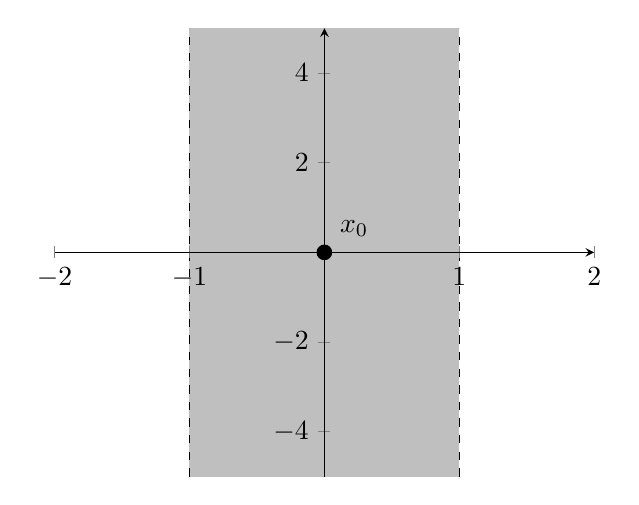
\begin{tikzpicture}
\begin{axis}[axis lines=middle, axis on top, xmin=-2, xmax=2, ymin= -5, ymax=5, samples=200]
\draw[dashed, name path = f] (axis cs:-1,-5) -- (axis cs:-1,5);
\draw[dashed, name path = g] (axis cs:1,-5) -- (axis cs:1,5);
\draw (axis cs:0,0) node[fill,circle, inner sep=2pt, minimum size=1pt, label={45:$x_0$}] {};
\addplot[gray!50] fill between[of=f and g];
\end{axis}
\end{tikzpicture}
\end{center}
\caption*{The open unit ball $B_{r=1}(x_0)$ centered at $x_0 = (0, 0)$ in the pseudometric space $(X,d)$. Note that $B_{r=1}(x_0) = B_{r=1}(x_0')$ for any $x_0' = (\xi_1', \xi_2') \in \mathbb{R}^2$ with $\xi_1' = 0$.}
\end{figure}
\end{exer}

\section{Normed Spaces, Banach Spaces}
\subsection{Vector Spaces: a Review}\label{vectorspace}

\begin{defn}[Vector space]
A \textbf{vector space} $V$ over a field $K$ is a nonempty set of elements called \textbf{vectors} together with two algebraic operations. The operations are \textbf{vector addition} and \textbf{multiplication of vectors by scalars}, that is, by elements of $K$.\newline
~\newline
\textbf{Vector addition} associates with every ordered pair of $(x, y) \subset V \times V$ of vectors a vector $x + y \in V$, called the \textbf{sum} of $x$ and $y$, in such a way that the following properties hold:
\begin{enumerate}
    \item $x + y = y + x$ \quad (commutativity)
    \item $x + (y + z) = (x + y) + z$  \quad (associativity)
\end{enumerate}
Furthermore, there exists a \textbf{zero vector} $\0 \in V$, the \textbf{additive identity}, which satisfies
\begin{align*}
    x + \0 = x \quad \forall x \in V.
\end{align*}
And for every vector $x$ there exists an \textbf{additive inverse}, $-x \in V$, which satisfies
\begin{align*}
    x + (-x) = \0.
\end{align*}
~\newline
\textbf{Multiplication by scalars} associates with every vector $x \in V$ and scalar $\alpha \in K$ a vector $\alpha x \in V$ called the \textbf{product} of $\alpha$ and $x$, in such a way that for all vectors $x, y \in V$ and scalars $\alpha, \beta \in K$
\begin{enumerate}
    \item $\alpha(\beta x) = (\alpha \beta)x$ \quad (associativity)
    \item $\alpha(x + y) = \alpha x + \alpha y$\newline $(\alpha + \beta)x = \alpha x + \beta x$ \quad (distributivity)
\end{enumerate}
Also, there exists a \textbf{multiplicative identity} element in the field $K$, $1 \in K$, which satisfies
\begin{align*}
    1x = x, \quad \forall x \in V.
\end{align*}
~\newline
If $K = \mathbb{R}$, then $V$ is called a \textbf{real vector space}. And if $K = \mathbb{C}$, then $V$ is called a \textbf{complex vector space}.
\end{defn}

\begin{thm}
Let $V$ be a vector space over the field $K$. Then the following hold for all vectors $x \in V$ and scalars $\alpha \in K$:
\begin{enumerate}
    \item $0x = \0$
    \item $\alpha \0 = \0$
    \item $(-1)x = -x$
\end{enumerate}
\end{thm}

\begin{examp}[The Euclidean vector space]\label{euclideanvector}
The set $V = \mathbb{R}^n$ with field $K = \mathbb{R}$ is a vector space with the following definitions of vector addition and scalar multiplication: for $x = (\xi_1, \ldots, \xi_n), y = (\eta_1, \ldots, \eta_n) \in \mathbb{R}^n$ and $\alpha \in \mathbb{R}$, 
\begin{align*}
    &x + y = (\xi_1 + \eta_1, \ldots, \xi_n + \eta_n)\\
    &\alpha x = (\alpha \xi_1, \ldots, \alpha \xi_n)
\end{align*}
\end{examp}

\begin{examp}[The unitary vector space]
The set $V = \mathbb{C}^n$ with field $K = \mathbb{C}$ is a vector space. The operations of vector addition and scalar multiplication are defined analogously to as in Example \ref{euclideanvector}.
\end{examp}

\begin{examp}
The set $V$ consisting of all real-valued, continuous functions on $[a, b] \subset \mathbb{R}$ is a vector space over the field $K = \mathbb{R}$. The operations of vector addition and scalar multiplication are defined as follows:
\begin{align*}
    &(x+y)(t) = x(t) + y(t)\\
    &(\alpha x)(t) = \alpha x(t), \quad t \in [a, b]
\end{align*}
\end{examp}
Other function spaces that are also vector spaces include
\begin{enumerate}
    \item $B(A)$, the vector space of all real-valued, bounded functions on a set $A \subseteq \mathbb{R}$
    \item The vector space of all differentiable functions on $\mathbb{R}$
    \item The vector space of all real-valued functions on $[a, b]$ that are integrable in some sense
\end{enumerate}

\begin{examp}
Recall from Example \ref{ellp} that $\ell^2$ consists of all (complex-valued) sequences $x = (\xi_1, \xi_2, \ldots)$ such that $\sum_{n=1}^{\infty} |\xi_n|^2 < \infty$, that is, $x$ is square summable. $\ell^2$ is a vector space over $K = \mathbb{C}$ with vector addition and scalar multiplication defined as follows:
\begin{align*}
    &(\xi_1, \xi_2, \ldots) + (\eta_1, \eta_2, \ldots) = (\xi_1 + \eta_1, \xi_2 + \eta_2, \ldots)\\
    &\alpha(\xi_1, \xi_2, \ldots) = (\alpha \xi_1, \alpha \xi_2, \ldots)
\end{align*}
The fact that $x + y \in \ell^2$ for $x, y \in \ell^2$ follows from the Minkowski inequality:
\begin{align*}
   \sum_{n=1}^{\infty} |\xi_n + \eta_n|^2 \leq \left( \left(\sum_{n=1}^{\infty} |\xi_n|^2 \right)^{1/2} + \left(\sum_{n=1}^{\infty} |\eta_n|^2 \right)^{1/2} \right)^2 < \infty.
\end{align*}
\end{examp}
Other sequence spaces that are also vector spaces include $\ell^{\infty}$ and $\ell^{p}$ for $1 \leq p < \infty$.

\begin{defn}[Subspace]\label{subspace}
A \textbf{subspace} of a vector space $X$ is a nonempty subset $Y$ of $X$ such that for all $y_1, y_2 \in Y$ and all scalars $\alpha, \beta \in K$, we have $\alpha y_1 + \beta y_2 \in Y$. Hence, $Y$ itself is a vector space, the two algebraic operations being induced from $X$.\newline
$Y = X$ is an \textbf{improper} subspace of $X$. Any other subspace of $X$ is called \textbf{proper}. $Y = \{\0\}$ is called the \textbf{trivial subspace}.
\end{defn}

\begin{defn}[Linear combination]\label{lincomb}
A \textbf{linear combination} of vectors $x_1, \ldots, x_n$ in a vector space $X$ over field $K$ is an expression of the form
\begin{align*}
    a_1 x_1 + a_2 x_2 + \ldots + a_n x_n, \quad a_1, a_2, \ldots, a_n \in K.
\end{align*}
It is important to note that linear combinations consist of \textit{finitely-many} vectors in $X$.
\end{defn}

\begin{defn}[Subspace spanned by a set]
For any nonempty subset $M \subset X$ the set of all linear combinations of vectors of $M$ is called the \textbf{span} of $M$, written
\begin{align*}
    \text{span} \ M.
\end{align*}
From Definition \ref{lincomb}, it should be apparent that for any $M$, $\text{span} \ M$ is a subspace. We call this subspace $Y$ the subspace \textbf{generated} by $M$.
\end{defn}

\begin{examp}\label{notlinear}
Consider the vector space $X$ of all sequences in $\mathbb{R}$ over the field $\mathbb{R}$. Define the subset $M$ of $X$ to be
\begin{align*}
  M = \bigcup_{i \in \mathbb{N}} e_i,  \qquad (e_i)_n = \begin{cases}
  1 & i = n\\
  0 & \text{otherwise}
  \end{cases}
\end{align*}
Then $\text{span} \ M \neq X$. To see why this is the case, consider any vector $x \in X$ with infinitely many nonzero terms. An example of such a vector is $x = (n^{-1})_{n \in \mathbb{N}}$. Then $x$ cannot be written as a (finite) linear combination of vectors in $X$. In fact, $\text{span} \ M$ is equal to the subspace consisting of all sequences with only finitely-many nonzero terms.
\end{examp}

\begin{defn}[Linear independence, dependence]
A (finite) set of vectors $\{x_1, \ldots, x_n\}$ is said to be \textbf{linearly independent} if 
\begin{align*}
    a_1 x_1 + a_2 x_2 + \ldots + a_n x_n = \0, \quad a_1, a_2, \ldots, a_n \in K \implies a_1 = a_2 = \ldots = a_n = 0.
\end{align*}
That is, the only representation of the zero vector by $x_1, \ldots, x_n$ is the trivial representation. If there exists a nontrivial representation of $\0$ by $x_1, \ldots, x_n$,
\begin{align*}
    a_1 x_1 + a_2 x_2 + \ldots + a_n x_n = \0, \quad x_i \neq 0, \ 1 \leq i \leq n,
\end{align*}
then the set of vectors $\{x_1, \ldots x_n\}$ is said to be \textbf{linearly dependent}.\newline
An arbitrary set of vectors $\boldsymbol{\beta}$ is said to be \textbf{linearly independent} if every nonempty finite subset of $\boldsymbol{\beta}$ is linearly independent.
\end{defn}
One should consider why the terms independent and dependent are used here. Specifically, if a set of vectors $\{x_1, \ldots, x_n \}$ is linearly dependent, then at least one vector $x_i, \ 1 \leq i \leq n$ can be written as a linear combination of the remaining vectors.

The notions of linear independence and dependence lead us to the following definition which tells us about the structure of a vector space $X$:
\begin{defn}[Basis]
A set of vectors $\boldsymbol{\beta}$ is a \textbf{basis} (or \textbf{Hamel basis}) for the vector space $X$ if
\begin{enumerate}
    \item $\boldsymbol{\beta}$ is linearly independent
    \item $\text{span} \ \boldsymbol{\beta} = X$
\end{enumerate}
\end{defn}

\begin{examp}
Let us consider the Euclidean vector space $\mathbb{R}^n$ over the field $\mathbb{R}$. Define $e_i \in \mathbb{R}^n, \ 1 \leq i \leq n$ such that
\begin{align*}
    (e_i)_j = \begin{cases}
    1 & \text{if $i = j$}\\
    0 & \text{otherwise}
    \end{cases}, \quad 1 \leq j \leq n.
\end{align*}
Then $(e_i)_{i=1}^n$ is a basis for $\mathbb{R}^n$. This basis is called the \textbf{canonical basis} for $\mathbb{R}^n$.
\end{examp}

\begin{examp}\label{notbasis}
Consider the vector space $X$ and the set $M$ defined in Example \ref{notlinear}. Then $M$ is \textbf{not} a basis for $X$.
\end{examp}

\begin{thm}\label{vectorbasis}
Every vector space $X \neq \{\0\}$ has a basis.
\end{thm}
Theorem \ref{vectorbasis} is surprising, especially in light of Example \ref{notbasis}.

\begin{thm}\label{basiselt}
Let $X$ be a vector space, and suppose $\boldsymbol{\beta}_1$ and $\boldsymbol{\beta}_2$ are two bases for $X$. Then $|\boldsymbol{\beta}_1| = |\boldsymbol{\beta}_2|$. This means that all bases for $X$ must have the same number of elements.
\end{thm}

\begin{defn}[Dimension]
The \textbf{dimension} of a vector space $X$ is the cardinality of any of its bases. As a consequence of Theorem \ref{basiselt}, the dimension is well-defined. If the dimension of a vector space $X$ is finite, then it is \textbf{finite-dimensional}. Otherwise, it is \textbf{infinite-dimensional}.
\end{defn}

\begin{thm}[Dimension of a subspace]
Let $X$ be an $n$-dimensional vector space. Then any proper subspace of $X$ has dimension less than $X$.
\end{thm}

\begin{exer}
Show that in an $n$-dimensional vector space $X$, the representation of any $x$ as a linear combination of given basis vectors $e_1, \ldots, e_n$ is unique.
\begin{proof}
Suppose towards contradiction that for an arbitrary $x \in X$ we have
\begin{align*}
    &x = a_1 e_1 + \ldots + a_n e_n\\
    &x = b_1 e_1 + \ldots + b_n e_n
\end{align*}
where $a_i \neq b_i$ for some $1 \leq i \leq n$. That is, $x$ has two distinct representations as a linear combination of basis vectors $e_1, \ldots, e_n$. This implies that
\begin{align*}
    &x + (-x) = (a_1 - b_1)e_1 + \ldots + (a_n - b_n)e_n\\
    &\0 = (a_1 - b_1)e_1 + \ldots + (a_n - b_n)e_n.
\end{align*}
But because $a_i \neq b_i$, then $a_i - b_i \neq 0$. And so we have expressed $\0$ as a nontrivial linear combination of vectors $e_1, \ldots, e_n$, and so the set of vectors $\{e_1, \ldots, e_n\}$ cannot cannot be linearly independent. Clearly, though, this contradicts our assumption that $\{e_1, \ldots, e_n\}$ is a basis for $X$.\newline
We conclude that each vector $x \in X$ must have a unique representation as a linear combination of $e_1, \ldots, e_n$.
\end{proof}
\end{exer}

\begin{exer}[The vector space of polynomials with degree at most $n$]
On a fixed interval $[a, b] \subset \mathbb{R}$, consider the set $X$ consisting of all polynomials with real coefficients and of degree not exceeding a given $n$, and the polynomial $x = 0$ (for which a degree is not defined in the usual discussion of degree). $X$ is a real vector space with the usual addition and the usual multiplication by real numbers. Find a basis for $X$, and then give the dimension of $X$. We can obtain a complex vector space $\tilde{X}$ in a similar fashion if we let those coefficients be complex. Is $X$ a subspace of $\tilde{X}$?\newline
A basis for the real vector space $X$ is $\{0, t^1, t^2, \ldots, t^n\}$, and so the dimension of $X$ is $n + 1$. $X$ is not a subspace of $\tilde{X}$ because the field over which $\tilde{X}$ is defined is $\mathbb{C}$. Thus, $X$ is not closed under scalar multiplication. For instance, $t + 3t^2 \in X$ but $i(t + 3t^2) \notin X$.
\end{exer}

\begin{exer}
If $Y$ and $Z$ are subspaces of a vector space $X$, show that $Y \cap Z$ is a subspace of $X$, but $Y \cup Z$ need not be one.\newline
We first show that $Y \cap Z$ is a subspace of $X$:
\begin{proof}
Let $x_1, x_2 \in Y \cap Z$ and $a_1, a_2 \in K$. Then because $x_1, x_2 \in Y$ and $Y$ is a subspace, $a_1 x_1 + a_2 x_2 \in Y$. The same holds for $Z$. Therefore, $a_1 x_1 + a_2 x_2 \in Y \cap Z$. Because vectors $x_1, x_2 \in Y \cap Z$ were chosen to be arbitrary, as were scalars $a_1, a_2 \in K$, this shows that $Y \cap Z$ is a subspace of $X$.
\end{proof}

Now, we show that $Y \cup Z$ need not be a subspace of the vector space $X$.\newline 
To do so, let us consider the Euclidean vector space $\mathbb{R}^2$ over the field $\mathbb{R}$. It is easy to verify that $Y = \{(x,y) \ | \ y = 2x\}$ and $Z = \{(x,y) \ | \ y = x\}$ are subspaces of $\mathbb{R}^2$. However, consider $(1, 2) \in Y$ and $(1, 1) \in Z$. Then $(1, 2) + (1, 1) = (2, 3) \notin Y \cup Z$. This counterexample shows that $Y \cup Z$ need not be a subspace of $X$.
\end{exer}

\begin{exer}[Quotient space, codimension]\label{quotientspace}
Let $Y$ be a subspace of a vector space $X$. The \textbf{coset} of an element $x \in X$ with respect to $Y$ is denoted by $x + Y$ and is defined to be
\begin{align*}
    x + Y := \{v \ | \ v = x + y, y \in Y \}.
\end{align*}
Show that the distinct cosets form a partition of $X$.
\begin{proof}
First, we show that every element $x \in X$ belongs to at least one coset. In particular, since $Y$ is a subspace, it must be true that $\0 \in Y$. Therefore, we have that $x = x + \0 \implies x \in x + Y$.\newline
It remains to show that each $x$ belongs to no more than one coset. Suppose that $v \in X$ satisfies $v \in x + Y$ as well as $v \in x' + Y$ for $x \neq x$. Then 
\begin{align*}
    &v = x + y, \quad v = x' + y'\\
    \iff& x + y = x' + y'\\
    \iff& x - x' = y' - y  \in Y.
\end{align*}
This, however, tells us $x = x' + y_0$ for some $y_0 \in Y$. And so $v = x + y = (x' + y_0) + y = x' + (y_0 + y)$, which implies $x + Y \subseteq x' + Y$. Also, the statement $y = x' + y_0$ implies $x' = x + (-y_0)$ for $(-y_0) \in Y$, and so $x + Y \supseteq x' + Y$. We deduce $x + Y = x' + Y$, meaning each $v \in X$ must belong to a unique coset. 
\end{proof}

Show that under the algebraic operations defined by
\begin{align*}
    &(w + Y) + (x + Y) = (w + x) + Y\\
    &\alpha(x + Y) = \alpha x + Y
\end{align*}
these cosets constitute the elements of a vector space.
\begin{proof}
    We begin by proving that the operations of addition and scalar multiplication are well-defined. In particular, we want to show that if $x + Y = x' + Y$ and $w + Y = w' + Y$, then $(x + w) + Y = (x' + w') + Y$ as well as $\alpha x + Y = \alpha x' + Y$.\newline
    For vector addition, notice that $x + Y = x' + Y \implies x = x' + y_1, \ y_1 \in Y$ as well as $w + Y = w' + Y \implies w = w' + y_2, \ y_2 \in Y$. Therefore, $v = (w + x) + y \implies  v = (x' + w') + (y_1 + y_2 + y)$, which tells us $(w + x) + Y \subseteq (w' + x') + Y$. The opposite direction of containment follows similarly.\newline
    And for scalar multiplication, once again we have  $x + Y = x' + Y \implies x = x' + y_1, \ y_1 \in Y$. Therefore, $v = \alpha x + y \implies v = \alpha x' + (\alpha y_1 + y)$, and so $\alpha x + Y \subseteq \alpha x' + Y$. By a similar argument we also get the opposite containment.\newline
    Now that we have shown that the operations of vector addition and scalar multiplication are well-defined, we prove that the cosets form a vector space. Note that the vector space is defined over the same field $K$ as that of $X$. \newline
    Commutativity follows from the commutativity of $X$: $(x + Y) + (w + Y) = (x + w) + Y = (w + x) + Y = (w + Y) + (x + Y)$. And associativity follows from the associativity of $X$: $((x + Y) + (w + Y)) + (z + Y) = ((x + w) + z) + Y = (x +( w + z)) + Y = (x + Y) + ((w + Y) + (z + Y))$.\newline
    The additive identity element is given by $\0 + Y$ since $(x + Y) + (\0 + Y) = (x + \0) + Y = x + Y$. The additive inverse of $x + Y$ is $(-x) + Y$ because $(x + Y) + (-x + Y) = (x + (-x)) + Y = \0 + Y$.\newline
    Similar to our arguments for commutativity and associativity, distributivity follows from that of the vector space $X$: $\alpha( (x + Y) + (w + Y)) = \alpha ((x + w) + Y) = (\alpha x + \alpha w) + Y = (\alpha x + Y) + (\alpha w + Y) = \alpha(x + Y) + \alpha (w + Y)$ and $(\alpha + \beta)(x + Y) = (\alpha + \beta)x + Y = (\alpha x + \beta x) + Y = (\alpha x + Y) + (\beta x + Y) = \alpha(x + Y) + \beta (x + Y)$.\newline
    The same is true for multiplicative associativity: $\alpha(\beta(x +Y)) = \alpha(\beta x + Y) = \alpha \beta x + Y = \beta \alpha x + Y = \beta (\alpha x + Y) = \beta(\alpha(x +Y))$.\newline
    Finally for $1 \in K$, we have $1(x + Y) = 1x + Y = x + Y$. \newline
    This proves that for a vector space $X$ defined over a field $K$ with subspace $Y$, the set of cosets of $X$ with respect to $Y$ forms a vector space over field $K$.
\end{proof}
This space is called the \textbf{quotient space} or \textbf{factor space} of $X$ by $Y$ and is denoted by $X/Y$. Its dimension is called the \textbf{codimension} of $Y$ and is denoted by $\text{codim} \ Y$, that is, 
\begin{align*}
    \text{codim} \ Y = \text{dim}(X/Y).
\end{align*}
\end{exer}

\begin{exer}
Let $X = \mathbb{R}^3$ and $Y = \{ (\xi_1, 0, 0) \ | \ \xi_1 \in \mathbb{R}\}$. Find $X/Y, X/X, X/\{\0\}$.\newline
Let $x = (\eta_1, \eta_2, \eta_3) \in \mathbb{R}^3$. For $X/Y$, we have that $x + Y = \{(\xi, \eta_2, \eta_3) \ | \ \xi \in \mathbb{R} \}$; that is, $x + Y$ is a line $\{ (0, \eta_2, \eta_3) + t(1, 0, 0) \ | \  t \in \mathbb{R} \}$. Because the direction vector of this line $(1, 0, 0)$ is equal to that of the $x$-axis, we deduce that $X/Y$ is the set of all lines that are parallel to the $x$-axis.\newline
For $X/X$, we have $x + X = \0_{X} + X = \0_{X/X}$. This is because $\{ v \ | \ v = x + y, y \in X \} = X$; for each $v \in X$, we can let $y = v + (-x) \in X$ so that $x + y = v$.\newline
And lastly we have $X/\{\0\} = X$. This is because $X + \{\0\} = \{ v \ | \ v = x + \0 \} = \{x\}$.
\end{exer}

\subsection{Normed Spaces, Banach Spaces}

\begin{defn}\label{normedbanach}
A \textbf{normed space} $X$ \textit{is a vector space} with a \textbf{norm} defined on it. A norm on a (real or complex) vector space $X$ is a real-valued function on $X$ whose value at $x \in X$ is denoted by $\|x\|$. A norm satisfies the following axioms for every $x, y \in X$ and $\alpha \in K$:
\begin{enumerate}
    \item $\| x \| \geq 0$
    \item $\| x \| = 0 \iff x = \0$
    \item $\| \alpha x \| = |\alpha| \|x\|$
    \item $\| x + y \| \leq \| x \| + \| y \|$ \quad (triangle inequality)
\end{enumerate}

A norm on $X$ defines a metric $d$ by
\begin{align*}
    d(x, y) := \| x - y\|, \qquad x, y \in X
\end{align*}
and is called the \textbf{metric induced by the norm}. The normed space defined is denoted by $(X, \| \cdot \|)$ or simply by $X$.

A \textbf{Banach space} is a normed space that is complete in the metric induced by the norm.
\end{defn}
Intuitively, the norm assigns a nonnegative length to each vector in the vector space $X$.

\begin{thm}[Reverse triangle inequality]\label{reversetriangle}
Let $X$ be a normed space. Then it holds that for every $x, y \in X$,
\begin{align*}
    |\|y\| - \|x\|| \leq \| y - x\|.
\end{align*}
\begin{proof}
By the the triangle inequality we have
\begin{align*}
    &\|y \| = \|y - x + x\| \leq \| y - x\| + \|x\|\\
    \iff&\|y \| - \| x\| \leq \| y - x\|.
\end{align*}
Similarly, by starting with $\|x\|$ instead, we have
\begin{align*}
    &\|x\| \leq \|x- y + y\| \leq \|y - x\| + \|y\|\\
    \iff&\| x\| - \| y \| \leq \|y - x\|.
\end{align*}
We conclude $| \|y\| - \|x\| | \leq \| y-x \|$.
\end{proof}
\end{thm}

\begin{thm}[Continuity of the norm]\label{normcontinuous}
The norm is continuous, that is, $x \longmapsto \| x\|$ is a continuous mapping of $(X, \| \cdot \|)$ into $\mathbb{R}$.
\begin{proof}
Let $d$ denote the metric induced by the norm $\| \cdot \|$, and let $\tilde{d}$ denote the Euclidean metric.
Suppose $x_0 \in X$ is an arbitrary vector. And take $\varepsilon > 0$ be arbitrary.\newline
Then by the reverse triangle inequality from Theorem \ref{reversetriangle}, we have that
\begin{align*}
    d(x, x_0) < \varepsilon \implies \tilde{d}(\| x\|, \| x_0\|) = \left| \|x\| - \| x_0 \| \right| \leq \| x - x_0\| = d(x, x_0) < \varepsilon.
\end{align*}
Because $\varepsilon > 0$ was taken to be arbitrary, this proves that $x \longmapsto \| x\|$ is continuous at $x_0 \in X$. And because $x_0$ was chosen to be an arbitrary vector, we conclude that the map $x \longmapsto \| x\|$ is continuous.
\end{proof}
\end{thm}

Now that we have defined a normed space and presented two fundamental results regarding normed spaces, we provide some examples. The first set of normed spaces will be familiar from our discussion of metric spaces in Section \ref{secmetric}. In particular, many of the metrics we discussed in this section can be obtained from a norm.
\begin{examp}[Euclidean space $\mathbb{R}^n$, unitary space $\mathbb{C}^n$]\label{euclideanunitarynorm}
The Euclidean space $\mathbb{R}^n$ and unitary space $\mathbb{C}^n$ were defined in Example \ref{euclideanunitary}. They are Banach spaces with norm defined by
\begin{align*}
    \| x \| = \left( \sum_{i=1}^n |\xi_i|^2 \right)^{1/2} = \sqrt{|\xi_1|^2 + \ldots + |\xi_n|^2}.
\end{align*}
This norm induces the metric
\begin{align*}
    d(x, y) = \| x - y\| = \sqrt{|\xi_1 - \eta_1|^2 + \ldots + |\xi_n - \eta_n|^2}.
\end{align*}
From Example \ref{euclideanunitarycomplete}, we know that the metric spaces $(\mathbb{R}^n, d)$ and $(\mathbb{C}^n, d)$ are complete, which justifies why the Euclidean and unitary spaces are Banach spaces.
\end{examp}

\begin{examp}[The sequence space $\ell^p$]
The space $\ell^p, \ 1 \leq p < \infty$ defined in Example \ref{ellp} is a Banach space with norm defined by
\begin{align*}
    \| x\| = \left( \sum_{i=1}^{\infty} |\xi_i|^p \right)^{1/p}.
\end{align*}
This norm induces the metric
\begin{align*}
    d(x, y) = \| x - y \| = \left( \sum_{i=1}^{\infty} |\xi_i - \eta_i| ^p \right)^{1/p}.
\end{align*}
\end{examp}

\begin{examp}[The sequence space $\ell^{\infty}$]
The space $\ell^{\infty}$ defined in Example \ref{ellinfty} is a Banach space with norm defined by
\begin{align*}
    \| x \| = \sup_{i \in \mathbb{N}} |\xi_i|.
\end{align*}
The norm induces the metric
\begin{align*}
    d(x, y) = \| x - y\| = \sup_{i \in \mathbb{N}} |\xi_i - \eta_i|.
\end{align*}
\end{examp}

\begin{examp}[The function space $C{[a, b]}$]
The space $C[a, b]$ defined in Example \ref{contfun} is a Banach space with norm given by
\begin{align*}
    \| x \| = \max_{t \in [a, b]} |x(t)|.
\end{align*}
The norm induces the metric
\begin{align*}
    d(x, y) = \| x - y \| = \max_{t \in [a, b]} |x(t) - y(t)|.
\end{align*}
\end{examp}

\begin{examp}[An incomplete normed space]
Let $X$ be the vector space consisting of all continuous, real-valued functions on $[0,1]$ over the field $K = \mathbb{R}$. Then $(X, \| \cdot \|)$ is a normed space with
\begin{align*}
    \|x\| := \int_0^1|x(t)| dt.
\end{align*}
However, one will recall from Example \ref{continuousincomplete} that the metric space $(X, d)$ is incomplete, where $d$ is the metric induced by $\| \cdot \|$. Therefore, $(X, \| \cdot \|)$ is not a Banach space.
\end{examp}

We already know from Section \ref{completingmetric} that every incomplete metric space can be completed, and so it is natural to ask the same question about incomplete normed spaces. The following example details an incomplete normed space that can be completed.
\begin{examp}[The function space $L^p{[a,b]}$]
The vector space $X$ of all continuous, real-valued functions on $[a, b]$ forms a normed space $(X, \| \cdot \|_p)$ for $p \geq 1$ with norm defined by
\begin{align*}
    \|x\|_p = \left( \int_a^b |x(t)|^p dt \right)^{1/p}.
\end{align*}
This normed space is not complete. Consider, for example, the Cauchy sequence proposed in Example \ref{continuousincomplete}. To prove that the Cauchy sequence does not converge, one must simply replace the metric from Example \ref{continuousincomplete} with that induced by the norm $\| \cdot \|_p$ and modify each term in the Cauchy sequence to be defined on $[a, b]$ rather than on $[0,1]$.\newline
In Theorem \ref{completionnorm}, however, we prove that this normed space $(X, \| \cdot \|_p)$ can be completed. The completion is denoted by $L^p[a, b]$ and is a Banach space. As we shall see in Theorem \ref{completionnorm}, the operations of the vector space $X$ can be extended to the completion of $X$.\newline
This is not the only way to construct the $L^p[a, b]$ spaces, though. For instance, let $\tilde{X}$ consist of all Lebesgue measurable functions $x$ on $[a, b]$ such that $|x|^p$ is Lebesgue integrable on $[a, b]$. And define the equivalence relation $\sim$ such that 
\begin{align*}
    x \sim y \iff \int_a^b |x(t) - y(t)|^p d\mu = 0.
\end{align*}
Here, $\mu$ denotes the Lebesgue measure on $\mathbb{R}$. Then $L^p[a, b]$ can equivalently be defined as $\tilde{X}/\sim$, the set of equivalence classes of $\tilde{X}$ under the equivalence relation $\sim$. 
\end{examp}

For our last example in this section, we present an example of a metric which cannot be obtained from a norm.
\begin{examp}
Recall the space $s$ in Example \ref{sequencespaces} which consists of all sequences (bounded or unbounded) in $\mathbb{C}$. We showed that $s$ is a metric space with metric $d$ defined
\begin{align*}
    d(x, y) := \sum_{n=1}^{\infty} \frac{1}{2^i} \frac{|\xi_n - \eta_n|}{1 + |\xi_n - \eta_n|}, \quad x = (\xi_n), y =(\eta_n) \in s.
\end{align*}
The metric $d$, however, cannot be obtained from a norm. This is a consequence of Theorem \ref{translationinvariant}. In particular, it is not in general true that $d(\alpha x, \alpha y) = |\alpha| d(x, y)$.
\end{examp}

\begin{thm}[Translation invariance]\label{translationinvariant}
A metric $d$ induced by a norm on a normed space $X$ satisfies the following for all $x, y, a\in X$ and $\alpha \in K$:
\begin{enumerate}
    \item $d(x + a, y + a) = d(x, y)$
    \item $d(\alpha x, \alpha y) = |\alpha| d(x, y)$
\end{enumerate}
\end{thm}
\begin{proof}
Let $(X, \| \cdot \|)$ be a normed space and $(X, d)$ the metric space with $d(x, y) = \| x - y\|$. Then it holds that
\begin{align*}
    d(x + a, y + a) = \| (x + a) - (y + a) \| = \| x - y\| = d(x, y)
\end{align*}
as well as
\begin{align*}
    d(\alpha x, \alpha y) = \| \alpha x - \alpha y\| = \| \alpha(x - y) \| = |\alpha| \| x - y\| = |\alpha| d(x,y).
\end{align*}
\end{proof}

\begin{exer}
Show that we may replace axiom (2) in Definition \ref{normedbanach} by 
\begin{align*}
    \| x \| = 0 \implies x = \0.
\end{align*}
Show that nonnegativity also follows from axioms (3) and (4).
\begin{proof}
First, we prove that $x = \0 \implies \|x\| = 0$. This is a simple consequence of axiom (3) since by taking $x = \0$ and $\alpha = 0$ we must have
\begin{align*}
    \|0\0\| = 0\|\0\| \iff \| \0\| = 0. 
\end{align*}
And for nonnegativity, we can invoke axioms (3) and (4) to say
\begin{align*}
    &\| x + (-x) \| \leq \| x \| + \| -x \| & \text{axiom (4)}\\
    \iff& \| x + (-x) \| \leq 2\|x \|  & \text{\text{axiom (3)}}\\
    \iff&\|\0\| \leq 2\|x\|\\
    \iff& 0 \leq \|x\|.
\end{align*}
\end{proof}
\end{exer}

\begin{exer}\label{euclideannorms}
There are several norms of practical importance on the vector space of ordered $n$-tuples from Example \ref{euclideanunitarynorm}, notably those defined by
\begin{enumerate}
    \item $\|x\|_1 = |\xi_1| + |\xi_2| + \ldots + |\xi_n|$
    \item $\|x\|_p = (|\xi_1|^p + |\xi_2|^p + \ldots + |\xi_n|^p)^{1/p}$, \quad $1 < p < \infty$
    \item $\|x\|_{\infty} = \max\{|\xi_1|, \ldots, |\xi_n| \}$
\end{enumerate}
In each case, verify that Definition \ref{normedbanach} is satisfied.
\begin{proof}
\begin{enumerate}
    \item By the definition of the complex modulus function $| \cdot |: \mathbb{C} \longrightarrow \mathbb{R}_+$, we know that $|\xi_i| \geq 0, \ 1 \leq i \leq n \implies \| x\|_1 \geq 0$, which proves nonnegativity. Also by the nonnegativity of the modulus function, we have $\| x \| = 0 \iff  | \xi | = 0, \ 1 \leq i \leq n \iff x = \0$, and so axiom (2) holds. For axiom (3), we have $\| \alpha x \|_1 = |\alpha \xi_1| + |\alpha \xi_2| + \ldots + |\alpha \xi_n| = \alpha (|\xi_1| + |\xi_2| + \ldots + |\xi_n|) = \alpha \| x \|_1$. Finally, the triangle inequality follows from that for the complex plane $\mathbb{C}$: $\| x + y \| = |\xi_1 + \eta_1| + |\xi_2 + \eta_2| + \ldots + |\xi_n + \eta_n| \leq (|\xi_1| + |\xi_2| + \ldots + |\xi_n|) + (|\eta_1| + |\eta_2| + \ldots + |\eta_n|) = \|x\| + \|y\|$. We conclude that $\|\cdot\|_1$ is a metric on $\mathbb{R}^n$ and $\mathbb{C}^n$.
    \item Axioms (1) and (2) follow similarly to as in our proof for $\| \cdot \|_1$: $|\xi_i| \geq 0, \ 1 \leq i \leq n \implies |\xi_1|^p + |\xi_2|^p + \ldots + |\xi_n|^p \geq 0 \implies \|x\|_p = (|\xi_1|^p + |\xi_2|^p + \ldots + |\xi_n|^p)^{1/p} \geq 0$ and $\|x\|_p = 0 \iff |\xi_1|^p + |\xi_2|^p + \ldots + |\xi_n|^p = 0 \iff |\xi_i| = 0, \ 1 \leq i \leq n \iff x = \0$. As for axiom (3), we have $\| \alpha x \|_p = (| \alpha \xi_1|^p + | \alpha \xi_2|^p + \ldots + |\alpha \xi_n|^p)^{1/p} = (\alpha^p(|\xi_1|^p + |\xi_2|^p + \ldots + |\xi_n|^p))^{1/p} = |\alpha|(|\xi_1|^p + |\xi_2|^p + \ldots + |\xi_n|^p)^{1/p} = |\alpha| \| x\|_p$. Finally, for axiom (4), the triangle inequality, we invoke the Minkowski inequality for finite sums: $\| x + y \|_p = (\sum_{i=1}^n |\xi_i + \eta_i|^p)^{1/p} \leq (\sum_{i=1}^n |\xi_i|^p)^{1/p} + (\sum_{i=1}^n |\eta_i|^p)^{1/p} = \|x\|_p + \|y\|_p$. Thus, $\| \cdot \|_p$ is a norm on $\mathbb{R}^n$ and $\mathbb{C}^n$.
    \item For axiom (1), we once again have $|\xi_i| \geq 0, \ 1 \leq i \leq n \implies \|x\|_{\infty} =  \max\{|\xi_1|, |\xi_2|, \ldots, |\xi_n|\} \geq 0$. And for axiom (2), $\|x\|_{\infty} = 0 \iff \max\{|\xi_1|, \ldots, |\xi_n|\} = 0 \iff |\xi_i| = 0, \ 1 \leq i \leq n \iff x = \0$. For axiom (3), $\| \alpha x \|_{\infty} = \max\{ |\alpha\xi_1|, |\alpha\xi_2|, \ldots, |\alpha\xi_n|\} = \max\{|\alpha||\xi_1|, |\alpha||\xi_2|, \ldots, |\alpha||\xi_n|\} = |\alpha| \max\{|\xi_1|, |\xi_2|, \ldots, |\xi_n|\} = |\alpha| \|x\|_{\infty}$. Finally for the triangle inequality we have $\| x + y \|_{\infty} = \max\{|\xi_1 + \eta_1|, |\xi_2 + \eta_2|, \ldots, |\xi_n + \eta_n|\}  \leq \max\{|\xi_1| + |\eta_1|, |\xi_2| + |\eta_2|, \ldots, |\xi_n| + |\eta_n|\} \leq  \max\{|\xi_1|, |\xi_2|, \ldots, |\xi_n|\} + \max\{|\eta_1|, |\eta_2|, \ldots, |\eta_n|\} = \|x\|_{\infty} + \|y\|_{\infty}$. Therefore, $\| \cdot \|_{\infty}$ is a norm defined on $\mathbb{R}$ and $\mathbb{C}$.
\end{enumerate}
\end{proof}
\end{exer}

\begin{exer}[Convex set, segment]
A subset $A$ of a vector space $X$ is said to be \textbf{convex} if
\begin{align*}
    x, y \in A \implies M = \{z \in X \ | \ z = \alpha x + (1-\alpha)y, \ 0 \leq \alpha \leq 1 \} \subseteq A.
\end{align*}
$M$ is called a \textbf{closed segment} with \textbf{boundary points} $x$ and $y$. Any other $z \in M$ is called an interior point of $M$. Show that the closed unit ball
\begin{align*}
    \tilde{B}_{r=1}(\0) = \{x \in X \ | \ \|x\| \leq 1\}
\end{align*}
in a normed space $X$ is convex.
\begin{proof}
Consider arbitrary vectors $x, y \in \tilde{B}_{r=1}(\0)$ as well as arbitrary $t \in [0, 1]$.\newline
Then $\|tx + (1-t)y\| \leq \|tx\| + \|(1-t)y\| = t\|x\| + (1-t)\|y\| \leq t + (1-t) = 1$. Notice that the final inequality follows from our assumption that $x, y \in \tilde{B}_{r=1}(\0)$. We deduce $\|tx + (1-t)y\| \leq 1 \implies tx + (1-t)y \in \tilde{B}_{r=1}(\0)$.\newline
And since $t \in [0, 1]$ was chosen arbitrarily, we conclude that the closed segment $M = \{z \in X \ | \ z = \alpha x + (1-\alpha)y, \ 0 \leq \alpha \leq 1 \}$ is contained in $\tilde{B}_{r=1}(\0)$. Finally, because  we chose $x, y \in X$ to be arbitrary, then we conclude that the closed unit ball $\tilde{B}_{r=1}(\0)$ is convex.
\end{proof}
\end{exer}

\begin{exer}
Show that the discrete metric space on a vector space $X \neq \{\0\}$ cannot be obtained from a norm.\newline
Suppose that $X$ is a nontrivial vector space. Then the discrete metric on $X$, which defines the metric space $(X, d)$, is not translation invariant. To see why this is the case, let $x \neq y$ be any pair of vectors in $X$. Then $d(\alpha x, \alpha y) = 1 \neq |\alpha| = |\alpha| d(x, y)$ for any $\alpha \notin \{0, \pm 1\}$. By the contrapositive to Theorem \ref{translationinvariant}, we conclude that the discrete metric $d$ cannot be induced by a norm on $X$.
\end{exer}

\begin{exer}[Bounded set]\label{boundednorm}
Show that a subset $M$ in a normed space $X$ is bounded if and only if there is a positive number $c$ such that $\|x\| \leq c$ for every $x \in M$.
\begin{proof}
$\implies$ Suppose that $M$ is an arbitrary bounded subset of $X$. Then there exists a $\delta(M) \in  \mathbb{R}_+$ such that $d(x, y) \leq \delta(M)$ for every $x, y \in M$. In particular, we can let $\delta(M) = \sup_{x, y \in M} d(x, y)$ be the diameter of $M$. Also, let $x' \in M$ be an arbitrary element of the set $M$. By the triangle inequality
\begin{align*}
    x \in M \implies \|x\| \leq  \| x- x'\| + \|x'\| \leq \delta(M) + \|x'\|.
\end{align*}
Therefore, for $c = \delta(M) + \|x'\| \in \mathbb{R}_+$ we obtain the desired result.
\newline$\impliedby$ Now we suppose that $\|x\| \leq c$ for every $x \in M$, where $c \in \mathbb{R}_+$. Let $x$ and $y$ be arbitrary elements of $M$. Once again by the triangle inequality, 
\begin{align*}
    d(x, y) = \|x-y\| \leq \|x\| + \|-y\| = \|x\| + \|y\| \leq 2c.
\end{align*}
This proves that $\sup_{x, y \in M} d(x, y) \leq 2c$, and so $M$ is a bounded subset of $X$.
\end{proof} 
\end{exer}

\subsection{Further Properties of Normed Spaces}

\begin{defn}[Subspace of a normed space]
A \textbf{subspace} $Y$ of a normed space $X$ is a subspace of $X$ considered as a vector space, with the norm obtained by restricting the norm on $X$ to the subset $Y$. This norm on $Y$ is \textbf{induced by} the norm on $X$. If $Y$ is closed in $X$, then $Y$ is called a closed subspace of $X$. 
\end{defn}

\begin{note}
A subspace of a Banach space is not necessarily a Banach space, only a normed space. The following theorem tells us exactly when this subspace will also be a Banach space.
\end{note}

\begin{thm}[Subspace of a Banach space]
A subspace $Y$ of a Banach space $X$ is complete if and only if the set $Y$ is closed in $X$.
\end{thm}
\begin{proof}
See Theorem \ref{closedcomplete}
\end{proof}

\begin{defn}[Convergent, Cauchy sequences in normed spaces]
From our definitions of convergent and Cauchy sequences in metric spaces (see Section \ref{convergencemetric}), we can analogously define convergent and Cauchy sequences in a normed space:
\begin{enumerate}
    \item A sequence $(x_n)$ in a normed space $X$ is \textbf{convergent} if there exists an $x \in X$ such that
    \begin{align*}
        \lim_{n \to \infty} \|x_n - x\| = 0.
    \end{align*}
    \item A sequence $(x_n)$ in a normed space $X$ is \textbf{Cauchy} if for every $\varepsilon > 0$, there exists a $N_{\varepsilon} \in \mathbb{N}$ such that 
    \begin{align*}
        n, m > N_{\varepsilon} \implies \|x_n - x_m\| < \varepsilon.
    \end{align*}
\end{enumerate}
\end{defn}

Frankly, this material repetitive and could have been excluded altogether. The following definition, though, cannot be related to (general) metric spaces since it uses vector addition defined on $X$.
\begin{defn}[Infinite series]\label{seriesconverge}
Let $(x_n)$ be a sequence in a normed space $X$. Then the \textbf{sequence of partial sums} $(s_n) \subset X$ associated with $(x_n)$ is defined such that
\begin{align*}
    s_n = x_1 + x_2 + \ldots + x_n, \qquad n \in \mathbb{N}.
\end{align*}
If this sequence $(s_n)$ converges in the normed space $X$,
\begin{align*}
    s_n \longrightarrow s \iff \|s_n - s\| \longrightarrow 0,
\end{align*}
then the \textbf{infinite series}
\begin{align*}
    \sum_{n=1}^{\infty} x_n = x_1 + x_2 + \ldots
\end{align*}
is said to \textbf{converge} or be \textbf{convergent}. The \textbf{sum of the series} is defined to be
\begin{align*}
    \sum_{n=1}^{\infty}x_n.
\end{align*}
\end{defn}

\begin{defn}[Absolute convergence]
Let $(x_n)$ be a sequence in a normed space $X$. Then if the series
\begin{align*}
    \sum_{n=1}^{\infty} \| x_n\|
\end{align*}
converges, the series $(x_n)$ is said to be \textbf{absolutely convergent}.
\end{defn}

The definitions of convergent and absolutely convergent series in a normed space $X$ leads us to the following theorem, which is important for understanding Banach spaces:
\begin{thm}\label{banachabsoluteconvergence}
A normed space $X$ is complete (is a Banach space) if and only if absolute convergence implies convergence.
\end{thm}
\begin{proof}
$\implies$ Let $X$ be a Banach space. And suppose that the series $\sum_{n=1}^{\infty} x_n$ converges absolutely. 

We wish to show that the series $\sum_{n=1}^{\infty} x_n$ converges. In order to do so, let us first define the $n$th partial sum of the aforementioned series, $s_n = x_1 + \ldots + x_n$. Also define the $n$th partial sum of  $\sum_{n=1}^{\infty} \|x_n\|$, $\tilde{s}_n = \|x_1\| + \ldots + \|x_n\|$. Take $\varepsilon > 0$ to be arbitrary. 

By assumption that $\sum_{n=1}^{\infty} x_n$ converges absolutely, there exists a $N_{\varepsilon} \in \mathbb{N}$ such that
\begin{align*}
    n, m > N_{\varepsilon}, n > m \implies |\tilde{s}_n - \tilde{s}_m| < \varepsilon \iff \|x_{m+1}\| + \ldots + \|x_n\| < \varepsilon.
\end{align*}
Therefore, by the triangle inequality, it holds that
\begin{align*}
    n, m > N_{\varepsilon}, n > m \implies \|s_n - s_m\|  = \| x_{m+1} + \ldots + x_n\| \leq \|x_{m+1}\| + \ldots + \|x_n\| < \varepsilon.
\end{align*}

Because $\varepsilon > 0$ was chosen to be arbitrary, we deduce that the sequence $(s_n)$ is Cauchy in the normed space $X$. And because $X$ is complete, then there exists an $s \in X$ such that $s_n \longrightarrow s$. Thus, by Definition \ref{seriesconverge}, the series $\sum_{n=1}^{\infty} x_n$ converges.

$\impliedby$ Conversely, suppose that $X$ is a normed space such that every absolutely convergent series in $X$ also converges in $X$. And let $(x_n)$ be an arbitrary Cauchy sequence in $X$. From this sequence $(x_n)$, we will construct a series that converges absolutely. 

By assumption that $(x_n)$ is Cauchy, for each $k \in \mathbb{N}$ we can find an $n_k \in \mathbb{N}$ such that
\begin{align*}
    n > n_k \implies \|x_n - x_{n_k}\| < 2^{-k}.
\end{align*}
In particular, this implies that we can find a subsequence $(x_{n_k})$ of $(x_n)$ such that for each $k \in \mathbb{N}$,
\begin{align*}
    \|x_{n_{k+1}} - x_{n_k}\| <  2^{-k}.
\end{align*}
From here, define $(y_k) \subset X$ such that $y_k := x_{n_{k+1}} - x_{n_k}$. We point out that we can define a sequence in this way since we are working on a vector space $X$ (as opposed to a metric space, for instance). 

We claim that $\sum_{k=1}^{\infty} y_k$ converges absolutely. To see why this is the case, notice that, by construction, $(\|y_k\|) = (a_k)$, where $a_k = 2^{-k}$. It is a well-known result from analysis that $a_k \longrightarrow 1$, and so we deduce that $\sum_{k=1}^{\infty} y_k$ converges absolutely.

Thus, by our assumption on the normed space $X$, $\sum_{k=1}^{\infty} y_k$ converges. This means that there exists an $x \in X$ such that 
\begin{align*}
    &\|s_k - x\| \longrightarrow 0 \iff \|(y_1 + \ldots + y_k) - x\| \longrightarrow 0 \iff \|x_{n_{k+1}} - x_{n_1} - x\| \longrightarrow 0\\
    &\|x_{n_{k+1}} - (x + x_{n_1})\| \longrightarrow 0.
\end{align*}
Here, $s_k = y_1 + y_2 + \ldots + y_k = (x_{n_2} - x_{n_1}) + (x_{n_3} - x_{n_2}) + \ldots + (x_{n_{k+1}} - x_{n_k}) = x_{n_{k+1}}  - x_{n_1}$ denotes the $k$th partial sum of $\sum_{i=1}^{\infty} y_i$. But because $(x_n)$ is Cauchy and has a convergent subsequence $x_{n_k} \longrightarrow (x + x_{n_1})$, then by Exercise \ref{cauchysubsequenceconvergent} we deduce that $x_n \longrightarrow (x + x_{n_1})$. 

$(x_n)$ is an arbitrary Cauchy sequence in $X$, and so we conclude $X$ is a Banach space.
\end{proof}

\begin{defn}[Schauder basis]
Let $X$ be a normed space. Suppose that $X$ contains a sequence $(e_n)$ with the property that for every $x \in X$, there exists a \textit{unique} sequence of scalars $(\alpha_n)$ such that
\begin{align*}
    \|(\alpha_1 e_1 + \ldots + \alpha_n e_n) - x\| \longrightarrow 0.
\end{align*}
Then $(e_n)$ is called a \textbf{Schauder basis} for $X$. The series
\begin{align*}
    \sum_{n=1}^{\infty} \alpha_n e_n
\end{align*}
is called the \textbf{expansion} of $x$ with respect to $(e_n)$, and we write
\begin{align*}
    x = \sum_{n=1}^{\infty}\alpha_n e_n.
\end{align*}
\end{defn}

\begin{examp}[A Schauder basis for $\ell^p$]
Consider the Banach space $\ell^p$ and define $(e_n)$ such that
\begin{align*}
    (e_n)_i = \begin{cases}
    1 & \text{if $i = n$}\\
    0 & \text{otherwise}
    \end{cases}, \quad i \in \mathbb{N}.
\end{align*}
That is, the $n$th term of $e_n$ is $1$ and all remaining terms are $0$. Then $(e_n)$ forms a Schauder basis for $\ell^p$.
\end{examp}

\begin{thm}
If a real or complex normed space has a Schauder basis, then it is separable.
\end{thm}
\begin{proof}
Let $X$ be a real normed space and suppose that $X$ has a Schauder basis $(e_n)$. Define the subset $M$ of $X$ such that 
\begin{align*}
    M := \bigcup_{n \in \mathbb{N}} \bigg\{ \sum_{i=1}^n \beta_i e_i  \ | \ \beta_i \in \mathbb{Q} \bigg\}.
\end{align*}
That is, $M$ consists of all linear combinations of the vectors $(e_n)$ with rational coefficients. We remark that $M$ is countable since each set $\{ \sum_{i=1}^n \beta_i e_i  \ | \ \beta_n \in \mathbb{Q} \}$ is countable.

Let $x \in X$ be arbitrary. And take $\varepsilon > 0$ to be arbitrary. Then because $(e_n)$ is a Schauder basis for $X$, there exists $\alpha_1, \ldots, \alpha_{N_{\varepsilon}}$ such that
\begin{align*}
    \|x - (\alpha_1 e_1 + \ldots + \alpha_{N_{\varepsilon}}e_{N_{\varepsilon}})\| < \frac{\varepsilon}{2}.
\end{align*}
Also, for each $1 \leq i \leq N_{\varepsilon}$, there exists a $\beta_i \in \mathbb{Q}$ such that 
\begin{align*}
    \|\beta_ie_i - \alpha_i e_i\| = |\beta_i - \alpha_i| \cdot \|e_i\| \leq \frac{\varepsilon}{2N_{\varepsilon}}.
\end{align*}
This implies that $m = \beta_1 e_1 + \ldots + \beta_{N_{\varepsilon}} e_{N_{\varepsilon}} \in M$ satisfies
\begin{align*}
    \|m - (\alpha_1 e_1 + \ldots + \alpha_{N_{\varepsilon}}e_n)\| \leq \|\beta_ie_i - \alpha_i e_i\| + \ldots + \|\beta_{N_{\varepsilon}} e_{N_{\varepsilon}} - \alpha_{N_{\varepsilon}} e_{N_{\varepsilon}}\| < \frac{\varepsilon}{2}
\end{align*}

Putting everything together, we have 
\begin{align*}
    \|m - x\| \leq \|m - (\alpha_1 e_1 + \ldots + \alpha_{N_{\varepsilon}}e_{N_{\varepsilon}})\| + \|(\alpha_1 e_1 + \ldots + \alpha_{N_{\varepsilon}}e_{N_{\varepsilon}}) - x\| < \varepsilon.
\end{align*}
That is, for each $\varepsilon > 0$, there exists a $m \in M$ such that $m \in B_{\varepsilon}(x)$. We conclude that $\bar{M} = X$, and so the normed space $X$ is separable.

For a complex normed space, the argument is exactly the same except for that we consider the $\beta_i$'s to be Gaussian rationals $\mathbb{Q}[i]$, which are dense in $\mathbb{C}$.
\end{proof}

To conclude this section of our notes, we prove that every (incomplete) normed space can be completed. 
\begin{thm}[Completion of a normed space]\label{completionnorm}
Let $X = (X, \|\cdot\|)$ be a normed space. Then there is a Banach space $\hat{X}$ and an isometry $A$ from $X$ onto a subspace $W$ of $\hat{X}$ which is dense in $\hat{X}$. The space $\hat{X}$ is unique, except for isometries. 
\end{thm}
\begin{proof}
By Theorem \ref{completion}, there exists a complete metric space $\hat{X} = (\hat{X}, \hat{d})$ and an isometry $A: X \longrightarrow W = A(X)$, where $W$ is dense in $\hat{X}$ and $\hat{X}$ is unique, except for isometries. Therefore, it remains to make $\hat{X}$ into a vector space and then introduce a suitable norm on $\hat{X}$.

Recall from Theorem \ref{completion} that the elements of $\hat{X}$ are the equivalence classes containing the Cauchy sequences of $X$ under the equivalence relation
\begin{align*}
    (x_n) \sim (y_n) \iff \lim_{n \to \infty} d(x_n, y_n) = 0.
\end{align*}
The metric defined on $\hat{X}$ is
\begin{align*}
    \hat{d}(\hat{x}, \hat{y}) = \lim_{n \to \infty} d(x_n, y_n),
\end{align*}
where $(x_n)$ and $(y_n)$ are representatives of the cosets $\hat{x}$ and $\hat{y}$, respectively.

For $(x_n) \in \hat{x}$ and $(y_n) \in \hat{y}$, let us define $(z_n)$ such that $z_n = x_n + y_n, \ n \in \mathbb{N}$. Observe that $(z_n)$ is indeed a Cauchy sequence since
\begin{align*}
    \|z_n - z_m\| \leq \|x_n - x_m\| + \|y_n - y_m\|.
\end{align*}
Therefore, let $\hat{z}$ denote the coset to which $(z_n)$ belongs. We can then define the operation of vector addition such that $\hat{x} + \hat{y} = \hat{z}$. This operation is independent of our choice of coset representatives, since for $(x_n') \in \hat{x}$,  $(y_n') \in \hat{y}$
\begin{align*}
    d(z_n, z_n') = \|z_n - z_n' \| = \|x_n - x_n'\| + \|y_n - y_n'\| \longrightarrow 0 \implies (z_n) \sim (z_n'). 
\end{align*}

We define scalar multiplication in a similar way. In particular let $(x_n) \in \hat{x}$ be an arbitrary coset representative, and define the sequence $(z_n)$ in $X$ such that $z_n = \alpha x_n, \ n \in \mathbb{N}$. $(z_n)$ is a Cauchy sequence because
\begin{align*}
    \|z_n - z_m\| = |\alpha|\|x_n - x_m\|.
\end{align*}
Let $\hat{z}$ be the coset to which the Cauchy sequence $(z_n)$ belongs. Then we define $\alpha \hat{x} = \hat{z}$. Just as was the case with vector addition, our definition of scalar multiplication does not depend upon which coset representative from $\hat{x}$ is chosen.

From here, it is easy to check that $\hat{X}$ is a vector space over the same field on which $X$ is defined. The additive identity element $\0_{\hat{X}}$ is the coset to which $A\0_{X}$ belongs (i.e. the coset which contains the constant sequence $(x_n), \ x_n = 0$).

Now to construct a norm on $\hat{X}$, we remark that the isometry $A$ induces on the set $W$ a norm $\|\cdot\|_1$. More specifically, we have
\begin{align*}
\|Ax\|_1 = \hat{d}(Ax, A\0_{X}) = d(x, \0_{X}) = \|x\|, \quad x \in X.
\end{align*}
The induced metric on $W$ by $\|\cdot\|_1$ is the restriction of $\hat{d}$ to $W$, as we would expect to be the case:
\begin{align*}
    \|Ax - Ay\|_1 = \|x - y\| = d(x, y) = \hat{d}(x, y).
\end{align*}

Finally, we must just extend the norm $\|\cdot\|_1$ to the entirety of $\hat{X}$. We do this by letting $\|\hat{x}\|_2 := \hat{d}(\0_{\hat{X}}, \hat{x}), \ \hat{x} \in X$. Notice that
\begin{align*}
\|Ax\|_2 = \hat{d}(\0_{\hat{X}}, A\hat{x}) = d(\0_{X}, x) = \|x\|,
\end{align*}
meaning that $\|\cdot\|_2$ is indeed equal to $\|\cdot\|_1$ on $W$. One can verify that $\|\cdot\|_2$ is indeed a valid norm on $\hat{X}$. It also remains to show that $W$ is dense in $\hat{X}$ in the metric induced by $\|\cdot\|_2$ (as opposed to in the metric $\hat{d}$, which we showed in our proof of Theorem \ref{completion}).
\end{proof}

\begin{exer}
Show that $x_n \longrightarrow x$ and $y_n \longrightarrow y$ implies $x_n + y_n \longrightarrow x + y$. Show that $\alpha_n \longrightarrow \alpha$ and $x_n \longrightarrow x$ implies $\alpha_n x_n \longrightarrow \alpha x$.
\begin{proof}
Fix $\varepsilon > 0$ to be arbitrary.\newline
Then there exists an $N_{\varepsilon}$ such that
\begin{align*}
    n >  N_{\varepsilon} \implies \|x_n - x\| < \frac{\varepsilon}{2}, \|y_n - y\| < \frac{\varepsilon}{2}.
\end{align*}
Therefore, we have that
\begin{align*}
    n >  N_{\varepsilon} \implies \| (x_n + y_n) - (x + y)\| \leq \| x_n - x\| + \|y_n - y\| < \varepsilon.
\end{align*}
This proves that $x_n + y_n \longrightarrow x + y$.\newline
For the second statement, suppose the field $K$ over which the vector space $X$ is defined is either the real line or complex plane. Let us consider the sequence $(\|x_n\|)$. In particular, since $x_n \longrightarrow x$ and $y \mapsto \|y\|$ is continuous (Theorem \ref{normcontinuous}), then by Theorem \ref{continuousmapping}, $\|x_n\| \longrightarrow \|x\|$. We deduce by Lemma \ref{uniquelimit} that $\sup_{n \in \mathbb{N}} \|x_n\| \leq c$ for some $c \in \mathbb{R}_{++}$ a constant. That is, the sequence $(\|x_n\|)$ is bounded. 

By assumption, there exists a $N_{\varepsilon} \in \mathbb{N}$ such that
\begin{align*}
    n > N_{\varepsilon} \implies |\alpha_n - \alpha| < \frac{\varepsilon}{2c}, \|x_n - x\| < \frac{\varepsilon}{2 \cdot \max\{1, |\alpha|\}}.
\end{align*}
Consequently, we have
\begin{align*}
    n > N_{\varepsilon} \implies \|\alpha_n x_n - \alpha x\| &\leq \|\alpha_n x_n - \alpha x_n\| + \| \alpha x_n - \alpha x\|\\
    &= |\alpha_n - \alpha| \|x_n\| + |\alpha| \|x_n - x\|\\
    &< \frac{\varepsilon}{2c} \cdot  c + |\alpha| \cdot \frac{\varepsilon}{2 \cdot \max\{1, |\alpha|\}}\\
    &\leq \varepsilon
\end{align*}
Note that we consider $\max\{1, |\alpha|\}$ as opposed to just $|\alpha|$ in order to avoid dividing by zero. This proves that $\alpha_n x_n \longrightarrow \alpha x$.
\end{proof}
\end{exer}

\begin{exer}
Show that the convergence of $\sum_{n=1}^{\infty} \|y_n\|$ may not imply the convergence of $\sum_{n=1}^{\infty} y_n$.\newline
Hint: Consider $Y$ to be the subspace of $\ell^{\infty}$ consisting of all sequences with only finitely-many nonzero terms. From Exercises \ref{subsetlinfty} and \ref{subsetlinftyclosed} we know that $Y$ is not a Banach space. And take $(y_n) \subset Y$ such that $y_n = \left(\eta_j^{(n)} \right)$, with $\eta_n^{(n)} = n^{-2}$ and $\eta_j^{(n)} = 0$ otherwise.

First, we point out that we need it to be the case that $Y$ is incomplete, since otherwise absolute convergence does imply convergence by Theorem \ref{banachabsoluteconvergence}. Now, we show that $(y_n)$ defined above does converge absolutely. Indeed, $\tilde{s}_n = \|y_1\| +\ldots +\|y_n\| = \sum_{i=1}^n \sup_{j \in \mathbb{N}}|\xi_j^{(i)}| = \sum_{i=1}^n i^{-2}$, and it is well-known from analysis that $\tilde{s}_n \longrightarrow \frac{\pi^2}{6}$. Therefore, the series $\sum_{n=1}^{\infty} y_n$ converges absolutely.

However, we claim that $\sum_{n=1}^{\infty} y_n$ does not converge. To see why this is the case, notice that the $n$th partial sum of the series, $s_n = y_1 + \ldots + y_n$, satisfies
\begin{align*}
    s_n = \left(\xi_j^{(n)} \right), \quad \xi_j^{(n)} = 
    \begin{cases}
    j^{-2} & \text{if $j \leq n$}\\
    0 & \text{otherwise}
    \end{cases}.
\end{align*}
And so in the Banach space $\ell^{\infty}$, $s_n \longrightarrow s$, where $s = (\xi_j)$ satisfies $\xi_j = j^{-2}$ for $j \in \mathbb{N}$. That is, when viewed as sequence in the Banach space $\ell^{\infty}$ (rather than in the normed space $Y$), $(s_n)$ converges to a vector $s$ which does not contain only finitely-many nonzero terms, and thus is not contained in $Y$. This then implies that $s_n$ is divergent in $Y$. Otherwise, we would violate the uniqueness of the limit of $(s_n)$ in $\ell^{\infty}$.
\end{exer}

\begin{exer}[Seminorm]\label{seminorm}
A \textbf{seminorm} on a vector space is a mapping $p: X \longrightarrow \mathbb{R}$ satisfying axioms (1), (3), and (4) in Definition \ref{normedbanach}. Show that 
\begin{align*}
    p(\0) = 0\\
    |p(x) - p(y)| \leq p(y-x).
\end{align*}
Thus, if $p(x) = 0$ implies $x = \0$, then $p$ is a norm.
\begin{proof}
By (3), for any $|\alpha| \neq 1$ we have $\|\alpha \0\| = |\alpha| \|\0\| \iff \|\0\|(1-|\alpha|) = 0 \implies \|\0\| = 0$.\newline
Now to prove the second statement, an analog of the reverse triangle inequality, we have
\begin{align*}
    &p(x) = p(x - y + y) \leq p(x-y) + p(y) & \text{axiom (4)}\\
    &p(x) - p(y) \leq p(x-y).
\end{align*}
Similarly,
\begin{align*}
    &p(y) = p(y - x + x) \leq p(y-x) + p(x) & \text{axiom (4)}\\
    &p(y) \leq p(x-y) + p(x) & \text{axiom (3)}\\
    &p(y) - p(x) \leq p(x-y). 
\end{align*}
Altogether, we conclude $|p(x) - p(y)| \leq p(x-y)$, as desired.

\end{proof}
\end{exer}

\begin{exer}
Let $Y$ be a closed subspace of a normed space $(X, \| \cdot \|)$. Show that a norm $\|\cdot\|_0$ on $X/Y$ is defined by
\begin{align*}
    \|\hat{x}\|_0 := \inf_{x \in \hat{x}} \|x\|, \qquad \hat{x} \in X/Y.
\end{align*}
\begin{proof}
The nonnegativity of the norm $\|\cdot\|_0$ follows directly from that of $\|\cdot\|$: 
\begin{align*}
    \|x\| \geq 0, \ \forall x \in X \implies \|\hat{x}\|_0 = \inf_{x \in \hat{x}}\|x\| \geq 0.
\end{align*}

Now, let $\0_{X/Y}$ be the zero coset. From Exercise \ref{quotientspace}, we know $\0_{X/Y} = \0_X + Y$, which implies $\0_X \in \0_{X/Y}$ because $Y$ is a subspace of $X$. Therefore,
\begin{align*}
    \|\0_{X/Y}\|_0 = \inf_{x \in \0_{X/Y}}\|x\| \leq \|\0_X\| = 0 \implies \|\0_{X/Y}\|_0 = 0.
\end{align*}
Conversely, suppose $\|\hat{x}\|_0 = 0$. By definition of $\|\cdot\|_0$, this implies that there exists a sequence $(x_n) \subset \hat{x}$ such that $\|x_n\| \longrightarrow 0_X$. By the definition of convergence in the normed space $X$, this implies $x_n \longrightarrow \0$. Finally, $Y$ closed implies that $\hat{x} = x_0 + Y$ , viewed as a set rather than element, is closed. This is the subject of the following lemma:

\begin{lm}
Let $Y$ be a closed subspace of a normed space $(X, \| \cdot \|)$. And let $\hat{x}$ be an arbitrary coset. Then $\hat{x}$ is closed when viewed as a subset of $X$. 
\end{lm}
\begin{proof}
Let $x_0$ be an arbitrary representative of the coset $\hat{x}$. Then we can write $\hat{x} = x_0 + Y = \{x_0 + y \ | \ y \in Y \}$. Let $x \in \bar{\hat{x}}$ be arbitrary. By Theorem \ref{closedconvergent}, there exists a sequence $(x_0 + y_n), \ y_n \in Y$ such that $x_0 + y_n \longrightarrow x$. And so 
\begin{align*}
    \|(x_0 + y_n) - x \| \longrightarrow 0 \iff  \|y_n - (x - x_0) \|  \longrightarrow 0  \iff y_n \longrightarrow x - x_0.
\end{align*}
But by assumption that $Y$ is closed, this means $x - x_0 \in Y$. Finally, writing $x = x_0 + (x - x_0)$, we deduce $x \in \hat{x}$.
\end{proof}

As a consequence, we have 
\begin{align*}
    x_n \longrightarrow \0_X, \ (x_n) \subset \hat{x} \implies \0_X \in \hat{x}.
\end{align*}
By Exercise \ref{quotientspace}, the cosets partition $X$, and so $\hat{x} =  \0_{X/Y}$.

For the third axiom, suppose $\hat{x} = x_0 + Y$. Then we have 
\begin{align*}
    \|\alpha \hat{x}\|_0 &= \inf_{x \in \alpha x_0 + Y} \|x\| = \inf_{y \in Y} \|\alpha x_0 +  y\|  = \inf_{y \in Y} \|\alpha x_0 +  \alpha y\| = |\alpha| \cdot \inf_{y \in Y} \|x_0 +  y\|\\
    &= |\alpha| \cdot \inf_{x \in x_0 + Y} \|x\| = |\alpha| \|\hat{x}\|_0.
\end{align*}
Note that the third equality holds because $Y$ is a subspace.

Finally, for the triangle inequality, let $\hat{x} = x_0 + Y$ and $\hat{y} = y_0 + Y$. Then it holds that
\begin{align*}
    \|\hat{x} + \hat{y}\|_0 &= \inf_{x \in (x_0 + y_0)  + Y}\|x \| = \inf_{y \in Y}\|(x_0 + y_0) + y\| \leq \inf_{y \in Y}( \|x_0 + y\| + \|y_0 + y\|)\\
    &\leq \inf_{y \in Y} \|x_0 + y\| + \inf_{y \in Y} \|y_0 + y\| = \|\hat{x}\|_0 + \|\hat{y}\|_0.
\end{align*}

We conclude that $\|\cdot\|_0$ is a norm on the quotient space $X/Y$.
\end{proof}
\end{exer}

\subsection{Finite-Dimensional Normed Spaces and Subspaces}

In this section, we restrict our attention to finite-dimensional normed spaces. That is, we consider normed spaces whose Hamel bases have finite cardinality.\footnote{Recall from Section \ref{vectorspace} that all Hamel bases of a given vector space have the same cardinality.}

We begin by presenting a result which shows \enquote{in the case of linear independence of vectors, we cannot find a linear combination that involves large scalars but represents a small vector}:
\begin{lm}\label{coeff}
Let $\{x_1, \ldots, x_n\}$ be a linearly independent set of vectors in a normed space $X$ (of any dimension). Then there is a $c \in \mathbb{R}_{++}$ such that for every choice of scalars $\alpha_1, \ldots, \alpha_n$,
\begin{align*}
    \|\alpha_1 x_1 + \ldots + \alpha_n x_n\| \geq c(|\alpha_1| + \ldots + |\alpha_n|).
\end{align*}
\end{lm}

As a consequence of this lemma, we get the following important theorem: 
\begin{thm}\label{finitecomplete}
Every finite-dimensional subspace $Y$ of a normed space $X$ is complete. In particular, every finite-dimensional normed space is complete.
\end{thm}
\begin{proof}
Let $(y_m)$ be an arbitrary Cauchy sequence in $Y$. Suppose that $\text{dim}\ Y = n$ and $\{e_1, \ldots, e_n\}$ is a Hamel basis for $Y$. Then we can write
\begin{align*}
    y_m = \alpha_1^{(m)}x_1 + \ldots + \alpha_n^{(m)}x_n, \qquad m \in \mathbb{N}. 
\end{align*}

Fix $\varepsilon > 0$ to be arbitrary. Because $(y_m)$ is a Cauchy sequence, then there exists a $N_{\varepsilon} \in \mathbb{N}$ such that
\begin{align*}
    n, m > N_{\varepsilon} \implies \left\|\sum_{j=1}^n (\alpha_j^{(n)} - \alpha_j^{(m)})e_i \right\| = \|y_n - y_m\| < \varepsilon.
\end{align*}
And by Lemma \ref{coeff}, there exists a $c \in \mathbb{R}_{++}$ such that $\|\sum_{j=1}^n \beta_j e_j\| \geq c\sum_{j=1}^n |\beta_j|$. Therefore, combining this with the previous statement, we get
\begin{align*}
    &n, m > N_{\varepsilon} \implies c|\alpha_j^{(n)} - \alpha_j^{(m)}| <  c\sum_{j=1}^n|\alpha_j^{(n)} - \alpha_j^{(m)}| < \varepsilon\\
    &n, m > N_{\varepsilon} \implies |\alpha_j^{(n)} - \alpha_j^{(m)}| < \frac{\varepsilon}{c}.
\end{align*}
And so for each $1 \leq j \leq n$, we have that $\left(\alpha_j^{(m)} \right) = (\alpha_j^{1}, \alpha_j^{2}, \ldots)$ is Cauchy sequence in $\mathbb{C}$ or $\mathbb{R}$. By Theorem \ref{realcomplete}, we have that both $\mathbb{C}$ and $\mathbb{R}$ are complete, and so $\alpha_j^{(m)} \longrightarrow \alpha_j$ for some $\alpha_j \in \mathbb{R}$. 

Using these limits, define 
\begin{align*}
    y = \alpha_1 e_1 + \ldots + \alpha_n e_n.
\end{align*}
We propose that $y$ is the limit of the Cauchy sequence $(y_m)$. First, because $Y$ is a subspace, then it must be true by Definition \ref{subspace} that $y \in Y$. Furthermore,
\begin{align*}
    \|y_m - y\| = \left\| \sum_{j=1}^n (\alpha_j^{(m)} - \alpha_j)e_j \right\| \leq \sum_{j=1}^n |\alpha_j^{(m)} - \alpha_j|\|e_j\|.
\end{align*}
Since $\alpha_j^{(m)} \longrightarrow a_j$, we can choose $N_{\varepsilon} \in \mathbb{N}$ such that $m > N_{\varepsilon} \implies |\alpha_j^{(m)} - \alpha_j| < \frac{\varepsilon}{n \cdot \max\{\|e_1\|, \ldots, \|e_n\|\}}$ for $1 \leq j \leq n$. This means
\begin{align*}
    m > N_{\varepsilon} \implies \|y_m - y\| \leq  \sum_{j=1}^n |\alpha_j^{(m)} - \alpha_j|\|e_j\| < \varepsilon.
\end{align*}

We deduce that $y_m \longrightarrow y$. Because $(y_m)$ was chosen to be an arbitrary Cauchy sequence in $Y$, then we conclude $Y$ is complete.
\end{proof}

As an immediate consequence of Theorem \ref{finitecomplete}, we get the following result:
\begin{thm}\label{finiteclosed}
Every finite-dimensional subspace $Y$ of a normed space $X$ is closed in $X$.
\end{thm}
\begin{proof}
Let $Y$ be a finite-dimensional subspace of a normed space $X$. By Theorem \ref{finitecomplete}, $Y$ is complete. And so by Theorem \ref{closedcomplete}, $Y$ is closed.
\end{proof}
\begin{note}
An infinite-dimensional subspace of a normed space need not be closed. Consider, for instance the subspace $\mathcal{P}$ of $C[a, b]$ consisting of all polynomials defined on the interval $[a, b] \subset \mathbb{R}$. By the Weierstrass approximation theorem, we know that $\bar{\mathcal{P}} = C[a, b]$ but $\mathcal{P} \neq C[a,b]$. That is, $\mathcal{P}$ is not closed in $C[a,b]$.
\end{note}

\begin{defn}[Equivalent norms]\label{equivalentnorms}
A norm $\|\cdot\|$ on a vector space $X$ is said to be \textbf{equivalent} to a norm $\|\cdot\|_0$ on $X$ if there are positive numbers $a, b$ such that for all $x \in X$ we have
\begin{align*}
    a\|x\|_0 \leq \|x\| \leq b\|x\|_0.
\end{align*}
\end{defn}
In Exercise \ref{equivalentnormstopology}, we prove that equivalent norms on $X$ define the same topology for $X$. That is, the open subsets of $X$ are the same, regardless of the choice of norm on $X$. We also prove in Exercise \ref{cauchyequivalentnorm} that the Cauchy sequences in $(X, \|\cdot\|)$ and $(X, \|\cdot\|_0)$ are the same.

The notion of equivalent norms leads us to the following theorem:
\begin{thm}\label{allequivalent}
On a finite-dimensional vector space $X$, any norm $\|\cdot\|$ is equivalent to any other norm $\|\cdot\|_0$.
\end{thm}
\begin{proof}
Let $\text{dim} \ X = n$ and $\{e_1, \ldots, e_n\}$ be a Hamel basis for $X$. Then for each $x \in X$, there is a unique representation of $x$ as a linear combination of $\{e_1, \ldots, e_n\}$:
\begin{align*}
    x = \alpha_1 e_1 + \ldots + \alpha_n e_n.
\end{align*}
By Lemma \ref{coeff}, there exists a $c \in \mathbb{R}_{++}$ such that
\begin{align*}
    \|x\| \geq c(|\alpha_1| + \ldots + |\alpha_n|).
\end{align*}
And letting $k = \max\{\|e_1\|_0, \ldots, \|e_n\|_0\}$, the triangle inequality gives us
\begin{align*}
    \|x\|_0 \leq \sum_{j=1}^n|\alpha_j| \|e_j\|_0 \leq k \sum_{j=1}^n|\alpha_j|.
\end{align*}
Therefore,
\begin{align*}
    \frac{1}{k}\|x\|_0 \leq \frac{1}{c}\|x\| \iff \frac{c}{k}\|x\|_0 \leq \|x\|.
\end{align*}

Now, let us interchange the role of $\|\cdot\|$ and $\|\cdot\|_0$. Namely, there exists a $c_1 \in \mathbb{R}_{++}$ such that
\begin{align*}
    \|x\|_0 \geq c_1 (|\alpha_1| + \ldots + |\alpha_n|).
\end{align*}
And letting $k_1 = \max\{\|e_1\|, \ldots, \|e_n\|\}$,
\begin{align*}
    \|x\| \leq \sum_{j=1}^n |\alpha_j| \|e_j\| \leq k_1 \sum_{j=1}^n |\alpha_j|.
\end{align*}
Thus,
\begin{align*}
    \frac{1}{k_1}\|x\| \leq \frac{1}{c_1}\|x\|_0 \iff \|x\| \leq \frac{k_1}{c_1} \|x\|_0
\end{align*}

We conclude
\begin{align*}
   \frac{c}{k} \|x\|_0 \leq \|x\| \leq \frac{k_1}{c_1} \|x\|_0,
\end{align*}
and so $\|\cdot\|$ and $\|\cdot\|_0$ are equivalent.
\end{proof}

Theorem \ref{allequivalent} implies that in a finite-dimensional vector space, the convergence or divergence of a sequence does not depend on the particular choice of norm on that space (see Exercise \ref{convergentequivalentnorm}).

\begin{exer}\label{equivalentnormsequivalencerelation}
Show that in Definition \ref{equivalentnorms}, the axioms of an equivalence relation hold.
\begin{proof}
Let $X$ be a vector space and suppose $\|\cdot\|, \|\cdot\|_1, \|\cdot\|_2$ are (arbitrary) norms on $X$.

First, notice that for all $x \in X$
\begin{align*}
    1\|x\| \leq \|x\| \leq 1\|x\|,
\end{align*}
which implies that $\|\cdot\| \sim \|\cdot\|$.

Next, suppose that $\|\cdot\| \sim \|\cdot\|_1$, meaning that there exists $a, b \in \mathbb{R}_{++}$ such that
\begin{align*}
    a\|x\|_1 \leq \|x\| \leq b\|x\|_1, \qquad x \in X.
\end{align*}
The first inequality implies that
\begin{align*}
    \|x\|_1 \leq \frac{1}{a}\|x\|, \qquad x \in X.
\end{align*}
And the second inequality tells us that
\begin{align*}
    \frac{1}{b}\|x\| \leq \|x\|_1, \qquad x \in X.
\end{align*}
Overall, we have
\begin{align*}
    \frac{1}{b}\|x\| \leq \|x\|_1 \leq \frac{1}{a}\|x\|, \qquad x \in X
\end{align*}
with $\frac{1}{b}, \frac{1}{a} \in \mathbb{R}_{++}$. This implies $\|\cdot\|_1 \sim \|\cdot\|$.

Finally, let us suppose $\|\cdot\| \sim \|\cdot\|_1$ and $\|\cdot\|_1 \sim \|\cdot\|_2$. Then there exist constants $a, b, a_1, b_1 \in \mathbb{R}_{++}$ such that 
\begin{align*}
    &a\|x\|_1 \leq \|x\| \leq b \|x\|_1\\
    &a_1\|x\|_2 \leq \|x\|_1 \leq b_1 \|x\|_2, \qquad &x \in X
\end{align*}
Notice that from the first inequality, $\|x\|_1 \leq \frac{1}{a}\|x\|$, and so by the second inequality
\begin{align*}
    a_1\|x\|_2 \leq \frac{1}{a}\|x\| \iff a_1a\|x\|_2 \leq \|x\|, \qquad x \in X.
\end{align*}
Similarly, the first inequality tells us $\frac{1}{b}\|x\| \leq \|x\|_1$ and so by the second inequality
\begin{align*}
    \frac{1}{b}\|x\| \leq b_1\|x\|_2 \iff \|x\| \leq b_1 b\|x\|_2, \qquad x \in X.
\end{align*}
Altogether,
\begin{align*}
    a_1a\|x\|_2 \leq \|x\| \leq b_1 b\|x\|_2, \qquad x \in X
\end{align*}
for $a_1a,  b_1 b \in \mathbb{R}_{++}$. And so $\|\cdot\| \sim \|\cdot\|_2$.

This proves that the definition of equivalent norms is an equivalence relation.
\end{proof}
\end{exer}

\begin{exer}\label{equivalentnormstopology}
Show that equivalent norms on a vector space $X$ induce the same topology on $X$.
\begin{proof}
Let $\|\cdot\|$ and $\|\cdot\|_0$ be two norms on the vector space $X$. 

We begin by outlining our argument. In particular, we will show that every open ball of radius $r > 0$ in $(X, \|\cdot\|)$ contains an open ball in $(X, \|\cdot\|_0)$ and vice versa. Taking this statement for given, let $A$ be an open set in $(X, \|\cdot\|)$; this means that we can write $A = \bigcup_{x \in A} B_{r_x}(x)$, where $B_{r_x}(x)$ is an open ball of radius $r_x > 0$ in $(X, \|\cdot\|)$. Because each $B_{r_x}(x)$ contains an open ball in $(X, \|\cdot\|_0)$, $B_{r_x'}^0(x)$, we can write $A = \bigcup_{x \in A} B_{r_x'}^0(x)$. Therefore, $A$ is open in $(X, \|\cdot\|_0)$ since it the union of open sets in $(X, \|\cdot\|_0)$. Proving that each open set in $(X, \|\cdot\|_0)$ is also open in $(X, \|\cdot\|)$ follows by the same argument.

Therefore, it only remains to show the inclusion of the open balls in $(X, \|\cdot\|)$ and $(X, \|\cdot\|_0)$.
Recall that because  $\|\cdot\|$ and $\|\cdot\|_0$ are equivalent, then there exists $a, b \in \mathbb{R}_{++}$ such that
\begin{align*}
    a\|x\|_0 \leq \|x\| \leq b \|x\|_0, \qquad x \in X.
\end{align*}

Let $B_r(x_0) = \{x \in X \ | \ \|x - x_0\| < r\}$ be an open ball in $(X, \|\cdot\|)$. Also, consider the open ball $B_{\frac{r}{b}}^0(x_0) = \{x \in X \ | \ \|x - x_0\|_0 < \frac{r}{b} \}$ in $(X, \|\cdot\|_0)$. Then
\begin{align*}
    x \in B_{\frac{r}{b}}^0(x_0) \implies \|x - x_0\| \leq b\|x - x_0\|_0 < r \implies x \in B_r(x_0).
\end{align*}
And so we conclude $B_{\frac{r}{b}}^0(x_0) \subseteq B_r(x_0)$.

Similarly, let $B_r^0(x_0) = \{x \in X \ | \ \|x - x_0\|_0 < r\}$ be an open ball in $(X, \|\cdot\|_0)$. And take the open ball $B_{ar}(x_0) = \{x \in X \ | \ \|x - x_0\| < ar\}$ in $(X, \|\cdot\|)$. Then
\begin{align*}
    x \in B_{ar}(x_0) \implies \|x - x_0\|_0 <\frac{1}{a}\|x - x_0\| < r \implies x \in B_r^0(x_0).
\end{align*}
And so we conclude $B_{ar}(x_0) \subset B_r^0(x_0)$.
\end{proof}

\begin{note}
One can also prove that if the topology induced on $X$ by $\|\cdot\|$ and $\|\cdot\|_0$ are the same, then $\|\cdot\|$ and $\|\cdot\|_0$ are equivalent.
\end{note}
\end{exer}

\begin{exer}\label{cauchyequivalentnorm}
If $\|\cdot\|$ and $\|\cdot\|_0$ are equivalent norms on $X$, show that the Cauchy sequences in $(X, \|\cdot\|)$ and $(X, \|\cdot\|_0)$ are the same.
\begin{proof}
Since $\|\cdot\|$ and $\|\cdot\|_0$ are equivalent norms, then there exist $a, b \in \mathbb{R}_{++}$ such that
\begin{align*}
    a\|x\| \leq \|x\|_0 \leq b\|x\|, \qquad x \in X.
\end{align*}
In particular, this implies that
\begin{align*}
    &a\|x - y\| \leq \|x - y\|_0 \leq b\|x - y\|, \qquad x, y \in X\\
    &ad(x, y) \leq d_0(x, y) \leq bd(x, y), \qquad x, y \in X.
\end{align*}
Here, $d$ and $d_0$ denote the metrics induced by the norms $\|\cdot\|$ and $\|\cdot\|_0$, respectively. 

By Exercise \ref{equivalentmetrics}, the Cauchy sequences in $(X, d)$ and $(X, d_0)$ are the same, which implies that the Cauchy sequences in $(X, \|\cdot\|)$ and $(X, \|\cdot\|_0)$ are the same.
\end{proof}
\end{exer}

\begin{exer}
Show that the norms $\|\cdot\|_1$ and $\|\cdot\|_2$ in Exercise \ref{euclideannorms} satisfy
\begin{align*}
    \frac{1}{\sqrt{n}}\|x\|_1 \leq \|x\|_2 \leq \|x\|_1.
\end{align*}
\begin{proof}
Let $x = (\xi_1, \ldots, \xi_n) \in \mathbb{C}^n$ be an arbitrary vector.

For the first inequality, we invoke the Cauchy-Schwarz inequality for $\mathbb{R}^n$:
\begin{align*}
    &\|x\|_1 = \sum_{i=1}^n |1 \cdot \xi_i| \leq \sqrt{\sum_{i=1}^n 1} \cdot \sqrt{\sum_{i=1}^n |\xi_i|^2} = \sqrt{n} \|x\|_2\\
    \implies& \frac{1}{\sqrt{n}}\|x\|_1 \leq \|x\|_2
\end{align*}

And for the second inequality,
\begin{align*}
    &\|x\|_2^2  = \sum_{i=1}^n |\xi_i|^2 \leq \left(\sum_{i=1}^n |\xi_i| \right)^2 = \|x\|_1^2\\
    \implies& \|x\|_2 \leq \|x\|_1
\end{align*}
The inequality on the first line follows from the multinomial theorem as well as the fact that each term in the sum  $\sum_{i=1}^n |\xi_i|$ is nonnegative.

Altogether, we conclude
\begin{align*}
    \frac{1}{\sqrt{n}}\|x\|_1 \leq \|x\|_2 \leq \|x\|_1, \qquad x \in X.
\end{align*}
\end{proof}
\end{exer}

\begin{exer}\label{convergentequivalentnorm}
If two norms $\|\cdot\|$ and $\|\cdot\|_0$ on a vector space $X$ are equivalent, show that 
\begin{align*}
    \|x_n -x\| \longrightarrow 0 \iff \|x_n -x\|_0 \longrightarrow 0.
\end{align*}
\begin{proof}
By Exercise \ref{equivalentnormsequivalencerelation}, it suffices to prove that
\begin{align*}
    \|x_n -x\| \longrightarrow 0 \implies \|x_n-x\|_0 \longrightarrow 0.
\end{align*}
Because $\|\cdot\|$ and $\|\cdot\|_0$ are equivalent, then there exists $a, b \in \mathbb{R}_{++}$ such that
\begin{align*}
    a \|x\|_0 \leq \|x\| \leq b\|x\|_0, \qquad x \in X.
\end{align*}

Fix $\varepsilon > 0$ to be arbitrary. Since $\|x_n -x\| \longrightarrow 0$, then there exists a $N_{\varepsilon} \in \mathbb{N}$ such that 
\begin{align*}
    n > N_{\varepsilon} \implies  \|x_n - x\| < a\varepsilon.
\end{align*}
Therefore, 
\begin{align*}
    n > N_{\varepsilon} \implies \|x_n - x\|_0 \leq \frac{1}{a}\|x_n - x\| < \varepsilon.
\end{align*}

Because $\varepsilon > 0$ was taken to be arbitrary, this proves $\|x_n - x\| \longrightarrow 0$.
\end{proof}

\begin{note}
The statement can be equivalently written as $x_n \longrightarrow x$ in $(X, \|\cdot\|)$ if and only if $x_n \longrightarrow x$ in $(X, \|\cdot\|_0)$.
\end{note}
\end{exer}

\subsection{Compactness and Finite Dimension}

\begin{defn}[Compactness]\label{compact}
A metric space $X = (X, d)$ is \textbf{compact} if for every collection of open sets $\mathcal{C}$ such that 
\begin{align*}
    X = \bigcup_{c \in \mathcal{C}} c
\end{align*}
then there exists a \textit{finite} subcollection of sets $\mathcal{F} \subseteq \mathcal{C}$ such that
\begin{align*}
    X = \bigcup_{f \in \mathcal{F}} f.
\end{align*}
More succinctly, $X$ is compact if each of its open covers has a finite subcover.
\end{defn}

\begin{defn}[Sequentially compact]\label{sequentiallycompact}
A metric space $X = (X, d)$ is \textbf{sequentially compact} if every sequence in $X$ has a convergent subsequence. A subset $M$ of $X$ is said to be compact if $M$ is compact considered as a subspace of $X$, that is, if every subsequence in $M$ has a convergent subsequence whose limit is in $M$.
\end{defn}

Although our definitions of compactness and sequential compactness may seem quite different, they are in fact equivalent when considering a metric space $X$:
\begin{thm}
Suppose that $X$ is a metric space. Then the following statements are equivalent:
\begin{enumerate}[(a)]
    \item $X$ is compact
    \item $X$ is sequentially compact
\end{enumerate}
\end{thm}
Therefore, from here on out we will refer to metric spaces that satisfy Definition \ref{sequentiallycompact} as compact.

Before proceeding, we take this opportunity to remind ourselves of two fundamental results from analysis that relate to compactness:
\begin{thm}[Heine-Borel]\label{heine-borel}
A subspace of the real line $(\mathbb{R}, d)$ is compact if and only if it is closed and bounded.
\end{thm}

\begin{thm}[Bolzano-Weierstrass]\label{bolzano-weierstrass}
Each bounded sequence on the real line $(\mathbb{R}, d)$ has a convergent subsequence.
\end{thm}

Now that we have done this, let us return to our discussion of compactness
\begin{lm}[Compactness]\label{compactclosedbounded}
A compact subset $M$ of a metric space $X = (X, d)$ is closed and bounded.
\end{lm}
\begin{proof}
Let $x \in \bar{M}$ be arbitrary. By Theorem \ref{closedconvergent}, there exists a sequence $(x_n) \subset M$ such that $x_n \longrightarrow x$. But by assumption that $M$ is compact, there is a subsequence $(x_{n_k})$ of $(x_n)$ that converges in $M$. And so because $(x_n)$ is convergent in $X$ with a convergent subsequence $(x_{n_k})$, then $(x_n)$ must converge to the same limit as $(x_{n_k})$. That is, we must have $x \in M$. We chose $x \in \bar{M}$ to be arbitrary, so we conclude $\bar{M} = M$, meaning $M$ is closed.

Now, suppose towards contradiction that $M$ is unbounded. That is, for any fixed element $m \in M$, $M$ contains a sequence $(x_n)$ such that $d(m, x_n) > n$. Since $M$ is compact, $(x_n)$ must have a convergent subsequence. This is impossible, though, because by Lemma \ref{uniquelimit} every convergent sequence must be bounded.
\end{proof}

\begin{note}
The converse to Lemma \ref{compactclosedbounded} is, in general, false.

As a counterexample, consider the following sequence $(x_n)$ in $\ell^2$. Define
\begin{align*}
    (x_n)_i := 
    \begin{cases}
    1 & i = n\\
    0 & \text{otherwise}
    \end{cases}, \qquad i \in \mathbb{N}.
\end{align*}
That is, the point $x_n$ has $1$ as its $n$th term and $0$ as all remaining terms. 

We claim that the point set $(x_n)$ is closed and bounded but not compact.  By Exercise \ref{boundednorm}, we know that $(x_n)$ is bounded because $\|x_n\| \leq 1$. And $(x_n)$ is closed because its only limit points are $x_n, \ n \in \mathbb{N}$. For the same reason, however, $M$ is not compact. 
\end{note}

\begin{defn}[Heine-Borel property]
A metric space $X = (X,d)$ has the \textbf{Heine-Borel property} if every closed and bounded subset $M$ of $X$ is compact.
\end{defn}
In the above note, we showed that $\ell^2$ does not have the Heine-Borel property.

\begin{thm}\label{heine-borel-property}
Every finite-dimensional normed space has the Heine-Borel property.
\end{thm}
\begin{proof}
Suppose $X = (X, \|\cdot\|)$ is a normed space with $\text{dim} \ X = n$ and Hamel basis $\{e_1, \ldots, e_n\}$. And choose $M \subset X$ to be any closed and bounded subset of $X$.

Let $(x_m)$ be an arbitrary sequence in $M$. Then by the definition of $\{e_1, \ldots, e_n\}$ a Hamel basis, there exists a unique representation
\begin{align*}
    x_m = \xi_1^{(m)} e_1 + \ldots + \xi_n^{(m)} e_n
\end{align*}
for each $m \in \mathbb{N}$. By assumption that the set $M$ is bounded, there exists a $k \in \mathbb{R}_+$ such that $\|x_m\| \leq k$ (Exercise \ref{boundednorm}). And by Lemma \ref{coeff}, there exists a $c \in \mathbb{R}_{++}$ such that
\begin{align*}
    &k \geq \|x_m\| = \left\| \sum_{i=1}^n \xi_i^{(m)} e_i \right\| \geq c\sum_{i=1}^n\left|\xi_i^{(m)}\right|\\
    \implies&\frac{k}{c} \geq \left|\xi_i^{(m)}\right|, \qquad i = 1, \ldots, n
\end{align*}

That is, for each $i = 1, \ldots, n$, the sequence $\left(|\xi_i^{(m)}| \right)$ is bounded in the Euclidean metric space. Therefore by the Bolzano-Weierstrass Theorem, there exists a subsequence $\left(|\xi_i^{(m_k)}| \right)$ of $\left(|\xi_i^{(m)}| \right)$ that converges to a limit $\xi_i$. Just as in the proof of Theorem \ref{coeff}, we conclude that there exists a subsequence $(z_m)$ of $(x_m)$ which converges to $z = \sum_{i=1}^n \xi_ie_i$. To see how one would explicitly construct this subsequence $(z_m)$, we encourage the reader to reference pp.~72-73 of Kreyszig. Lastly, by assumption that $M$ is closed, then $z_m \longrightarrow z \implies z \in M$. 

Therefore, we have proven that for an arbitrary sequence $(x_m)$ in the closed, bounded set $M$, then there exists a subsequence $(z_m)$ of $(x_m)$ such that $z_m \longrightarrow z$. We conclude that $M$ is compact. 

Because $M$ was chosen to be an arbitrary closed and bounded subset of $X$, this proves that $(X, \|\cdot\|)$ has the Heine-Borel property.
\end{proof}
As a consequence of Theorem \ref{heine-borel-property}, we have that in the Euclidean normed space $(X, \|\cdot\|)$, the compact sets are exactly the closed and bounded subsets. 

\begin{lm}[Riesz's Lemma]\label{rieszlemma}
Let $Y$ and $Z$ be subspaces of a normed space $X$ (of any dimension), and suppose $Y$ is closed and is a proper subset of $Z$. Then for every $\theta \in (0,1)$, there is a $z \in Z$ such that
\begin{align*}
    \|z\| = 1, \qquad \|z - y\| \geq \theta, \ \forall y \in Y
\end{align*}
\end{lm}

In a finite-dimensional normed space, the closed unit ball is compact by Theorem \ref{heine-borel-property}. Riesz's Lemma allows us to prove the converse:
\begin{thm}[Finite dimension]
If a normed space $X$ has the property that the closed unit ball $M = \{x \ | \ \|x\| \leq 1\}$ is compact, then $X$ is finite-dimensional.
\end{thm}
\begin{proof}
Suppose towards contradiction that $M$ is compact but $\text{dim}\ X = \infty$. Choose any $x_1 \in X$ with $\|x_1\| = 1$. Then $X_1 = \text{span}\{x_1\}$ is a one-dimensional subspace of $X$, and thus is closed by Theorem \ref{finiteclosed}. Also, since $\text{dim} \ X = \infty$, we know $X_1$ is a proper subspace of $X$.

Therefore, invoking Riesz's lemma with $Y = X_1$ and $Z = X$, there is an $x_2 \in X$ with $\|x_2\| = 1$ such that
\begin{align*}
    \|x_2 - x_1\| \geq \frac{1}{2}.
\end{align*}
The elements $x_1, x_2$ generate a two-dimensional proper, closed subspace $X_2$ of $X$.

Once again by Riesz's lemma, there is an $x_3$ satisfying $\|x_3\| = 1$ such that for all $x \in X_2$,
\begin{align*}
    \|x_3 - x\| \geq \frac{1}{2}.
\end{align*}
In particular,
\begin{align*}
    &\|x_3 - x_1\| \geq \frac{1}{2},\\
    &\|x_3 - x_2\| \geq \frac{1}{2}.
\end{align*}

Proceeding by induction, we obtain a sequence $(x_n)$ of elements $x_n \in M$ such that
\begin{align*}
    \|x_m - x_n\| \geq \frac{1}{2} \quad m \neq n.
\end{align*}
Clearly, $(x_n)$ cannot have a convergent subsequence. However, this contradicts our assumption that $M$ is compact.

Hence, we conclude $\text{dim} \ X < \infty$.
\end{proof}

Another important property of compact sets is that they are preserved under continuous maps:
\begin{thm}\label{continuouscompact}
Let $X$ and $Y$ be metric spaces and $T: X \longrightarrow Y$ a continuous mapping. Then the image of a compact subset $M$ of $X$ under $T$ is also compact.
\end{thm}
\begin{proof}
By the definition of $T(M)$ compact, we must show that for every sequence $(y_n) \subset T(M)$, there exists a subsequence $(y_{n_k})$ of $(y_n)$ that converges. Because $(y_n) \subset T(M)$, then there exists a sequence $(x_n) \subset M$ such that $y_n = Tx_n$ for each $n \in \mathbb{N}$. But because the sequence $(x_n)$ is contained in the compact set $M$, there exists a subsequence $(x_{n_k})$ such that $x_{n_k} \longrightarrow x$ for $x \in M$. Finally, by Theorem \ref{continuousmapping}, $T$ continuous and $x_{n_k} \longrightarrow x$ implies $y_{n_k} = Tx_{n_k} \longrightarrow Tx$. 

And so we have shown there exists a subsequence $(y_{n_k})$ of $(y_n)$ with $y_{n_k} \longrightarrow Tx$, where $x \in M \implies x \in T(M)$. Because $(y_n) \subset T(M)$ was chosen to be arbitrary, we conclude $T(M)$ is a compact subset of $Y$.
\end{proof}

Lastly, we prove a generalization of the Weierstrass Extreme Value Theorem. In order to do so, we first prove the following lemma:
\begin{lm}\label{infsup}
Suppose $A \subset \mathbb{R}$ is closed and bounded. Then $\sup A, \inf A  \in A$.
\end{lm}
\begin{proof}
First, if $A$ is empty, then $\sup A$ and $\inf A$ do not exist. Therefore, assume that $A$ is nonempty.

By assumption that $A$ is bounded, we have that $\sup A, \inf A \in \mathbb{R}$. Otherwise, it is possible $\sup A = +\infty$, $\inf A = -\infty$.

We first begin with $\sup A$. By the definition of the supremum, for every $n \in \mathbb{N}$ we can find an element $a_n \in A$ such that $\sup A - \frac{1}{n} < a_n \leq \sup A$. And so let us consider the sequence $(a_n)$. It is easy to see that $a_n \longrightarrow \sup A$. But $A$ is closed, which implies $\sup A \in A$.

We use a similar argument for $\inf A$. Namely, we construct the sequence $(a_n') \subset A$ such that $\inf A \leq a_n' < \inf A + \frac{1}{n}$ for each $n \in \mathbb{N}$. Then $a_n' \longrightarrow \inf A$. And $A$ closed implies $\inf A \in A$.
\end{proof}

Now, we are ready to prove the main result:
\begin{thm}
A continuous mapping $T$ of a compact subset $M$ of a metric space $X$ into $\mathbb{R}$ assumes a maximum and a minimum at some points of $M$.
\end{thm}
\begin{proof}
By Theorem \ref{continuouscompact}, the image of $M$ under the continuous map $T$, $T(M)$ is compact, and so by Lemma \ref{compactclosedbounded} it is closed and bounded. Further, by Lemma \ref{infsup} we have $\sup T(M), \ \inf T(M) \in T(M)$. The points in $M$ at which $T$ is maximized and minimized are $T^{-1}\sup T(M)$ and $T^{-1}\inf T(M)$, respectively.
\end{proof}

\begin{exer}\label{euclideannotcompact}
Show that $\mathbb{R}^n$ and $\mathbb{C}^n$ are not compact.\newline
Let $(\mathbb{C}^n, d)$ be the unitary metric space and consider the sequence $(x_n)$ defined 
\begin{align*}
    (x_n)_i := \begin{cases}
    n & \text{if $i = 1$}\\
    0 & \text{otherwise}
    \end{cases}, \quad 1 \leq i \leq n.
\end{align*}
That is, the first coordinate of the $n$th term in the sequence is equal to $n$, and and all other coordinates are zero. It is evident that $(x_n)$ does not have any limit points, though, and so it cannot have a convergent subsequence. This implies that $\mathbb{R}^n$ and $\mathbb{C}^n$ are not compact.
\end{exer}

\begin{exer}[Local Compactness]\label{locallycompact}
A metric space $X$ is said to be locally compact if every point of $X$ has a compact neighborhood. Show that $\mathbb{R}$ and $\mathbb{C}$ and, more generally, $\mathbb{R}^n$ and $\mathbb{C}^n$ are locally compact.
\begin{proof}
We prove the result for $\mathbb{C}^n$, although the proof is identical for $\mathbb{R}^n$. Let $x_0 \in \mathbb{C}^n$ be an arbitrary point. And consider the closed ball with unit radius centered at $x_0$, $\tilde{B}_{r =1}(x_0) = \{x \in \mathbb{C}^n \ | \ \|x - x_0\| \leq 1\}$. By Theorem \ref{heine-borel-property}, since the normed space $\mathbb{C}^n$ is finite-dimensional, it has the Heine-Borel property. Thus, $\tilde{B}_{r =1}(x_0)$ closed and bounded implies $\tilde{B}_{r =1}(x_0)$ compact. We deduce $x_0$ has a compact neighborhood. And because $x_0$ was chosen to be arbitrary, then every point of $\mathbb{C}^n$ has a compact neighborhood. We conclude $\mathbb{C}^n$ is locally compact.
\end{proof}
\end{exer}

\begin{exer}
Show that a compact metric space $X$ is locally compact.
\begin{proof}
This result is trivial. Let $x \in X$ be an arbitrary point. Then $X$ itself is a neighborhood of $x$ because $B_{r=1}(x) \subset X$. This is true for any point $x \in X$, and so we conclude $X$ is locally compact.
\end{proof}
\begin{note}
Be careful--the converse to this statement is not generally true. Consider, for instance, the Euclidean normed space $X = \mathbb{R}^n$. As we demonstrated in Exercise \ref{locallycompact}, $X$ is locally compact. But as we also know from Exercise \ref{euclideannotcompact}, $X$ is not compact.
\end{note}
\end{exer}

\begin{exer}
If $\text{dim} \ Y < \infty$ in Lemma \ref{rieszlemma}, show that one can even choose $\theta = 1$.
\begin{proof}
Let $e_1, \ldots, e_n$ be a Hamel basis for $Y$. Also, take $v \in Z\setminus Y$ be an arbitrary element. Then because $Y$ is closed, we must have $a := \inf_{y \in Y}\|y - v\| > 0$. Otherwise, we would have a sequence $(y_k')$ that satisfies $\|y_k' - v\| \longrightarrow 0 \implies y_k' \longrightarrow v$, meaning $v \in Y$.

Now, by the definition of the infimum, there exists a sequence $(y_k)$ in $Y$ which satisfies $\|y_k - v\| \longrightarrow a$. Notice that the sequence $(\|y_k - v\|)$ is convergent, and so it is bounded (Lemma \ref{uniquelimit}). Therefore,
\begin{align*}
    &l \geq \|y_k - v\| \geq | \|y_k\| - \|v\| | \geq \|y_k\| - \|v\|\\
    \implies&l' := l + \|v\| \geq \|y_k - v\| + \|v\| \geq \|y_k\|,
\end{align*}
which means that the sequence $(y_k)$ is also bounded.

Since $e_1, \ldots, e_n$ is a Hamel basis for $Y$, we can write
\begin{align*}
    y_k = \xi_1^{(k)}e_1 + \ldots + \xi_n^{(k)}e_n.
\end{align*}
And so by combining our previous result with Lemma \ref{coeff}, there exists a $c > 0$ such that
\begin{align*}
    &l' \geq \|y_k\| \geq c\sum_{i=1}^n \left|\xi_i^{(k)} \right|\\
    \implies&\frac{l'}{c} \geq \left|\xi_i^{(k)} \right|, \quad i = 1, \ldots, n.
\end{align*}
That is, we have shown each sequence $\left( \xi_i^{(k)}  \right)$, $i = 1, \ldots, n$ is bounded on the real line. Therefore, by the Bolzano-Weierstrass Theorem (Theorem \ref{bolzano-weierstrass}) for each $i = 1, \ldots, n$ there is a subsequence $\left( \xi_{i_p}^{(k)} \right)$ with $\xi_{i_p}^{(k)} \longrightarrow \xi_i$.

Using these $n$ individual sequences $\left( \xi_{i_p}^{(k)} \right)$, we can construct a subsequence $(y_{k_p})$ of $(y_k)$ such that $y_{k_p} \longrightarrow \tilde{y}$, where
\begin{align*}
    \tilde{y} = \xi_1 e_1 + \ldots + \xi_n e_n.
\end{align*}
Because $Y$ is closed, we know that $\tilde{y} \in Y$. Also, invoking the triangle inequality, we have
\begin{align*}
    \|\tilde{y} - v\| \leq \|\tilde{y} - y_{k_p}\| + \|y_{k_p} - v\| = \sum_{i=1}^n\underset{\longrightarrow0}{|\xi_i^{(k_p)} - \xi_i|} \|e_i\| + \underset{\longrightarrow a}{\|y_{k_p} - v\|}.
\end{align*}
And so $\|\tilde{y} - v\| \leq a \implies \|\tilde{y} - v\| = a$. That is, we have shown that the distance of $Y$ to $v$ is attained by some element $\tilde{y} \in Y$.

To complete the proof, let us define the unit vector
\begin{align*}
    z = a^{-1}(v - \tilde{y})
\end{align*}
And so for every $y \in Y$,
\begin{align*}
    \| y - z\| &= \|y - a^{-1}(v  - \tilde{y})\|\\
    &= a^{-1}\| ay - (v - \tilde{y})\|\\
    &= a^{-1}\|y_1 - v\|
\end{align*}
where
\begin{align*}
    y_1 = ay + \tilde{y}.
\end{align*}
Clearly, since $Y$ is a subspace, then $y_1 \in Y$. And so by the definition of $a$, $y_1 \in Y \implies \|y_1 - v\| \geq a$. We deduce
\begin{align*}
    \|y - z\| = a^{-1}\|y_1 - v\| \geq \frac{a}{a}= 1.
\end{align*}
\end{proof}
\end{exer}

\begin{exer}\label{closedcompact}
If $X$ is a compact metric space and $M \subset X$ is closed, show that $M$ is compact.
\begin{proof}
Let $(x_n)$ be an arbitrary sequence in $M$, where the metric is that induced by $X$. Since $X$ is compact, there exists a subsequence $(x_{n_k})$ of $(x_n)$ such that $x_{n_k} \longrightarrow x$ for some $x \in X$. But $M$ is closed, meaning it contains all of its limit point. That is, $(x_{n_k}) \subset M$ and $x_{n_k} \longrightarrow x$ implies $x \in M$. Because $(x_n)$ was chosen to be arbitrary, we conclude that $M$ is compact.
\end{proof}
\end{exer}

\begin{exer}
Let $X$ and $Y$ be metric spaces, $X$ compact, and $T: X \longrightarrow Y$ bijective and continuous. Show that $T$ is a homeomorphism.
\begin{proof}
Recall from Theorem \ref{continuousmapping} that $T^{-1}: Y \longrightarrow X$ is continuous if and only if the inverse image of any open set (in $X$) is open (in $Y$). Equivalently, $T^{-1}$ is continuous if and only if the inverse image of any closed set is closed. This is because, definitionally, the complement of any open set is closed and vice versa. And so it suffices to show that the inverse image of a closed set under $T^{-1}$ is closed.

Therefore, let $A \subseteq X$ be an arbitrary closed set. By Exercise \ref{closedcompact}, we know that $X$ compact and $A$ closed implies $A$ compact. Also, by the Theorem \ref{continuouscompact}, since $(T^{-1})^{-1} = T$ is continuous and $A$ is compact, then $(T^{-1})^{-1}(A) = T(A)$ is a compact subset of $Y$. Finally, by Lemma \ref{compactclosedbounded}, $(T^{-1})^{-1}(A)$ compact implies $(T^{-1})^{-1}(A)$ closed. Since $A$ was chosen to be an abitrary closed set in $X$, this proves that the inverse image of any closed set in $X$ under $T^{-1}$ is also closed. Thus, $T^{-1}$ is continuous.
\end{proof}
\end{exer}


\subsection{Linear Operators}

\end{document}